
In the last few years, I have contributed to a project to help make results published by CMS and ATLAS more accessible to theorists working outside the collaborations. The LPSC in Grenoble, the institution where the project is based, generously hosted me for periods of a few weeks to a month during the summers of 2013, 2014, and 2015. The following is a selection from the paper~\cite{Dumont:2014tja}.


\section{Toward a public analysis database for LHC new physics searches using \ma}
It is a challenge and in cases impossible for the broader community of physicists, namely theorists,
 to work out the implications of the LHC results 
in the context of all these different models, to derive the relevant limits, point out  
possible loopholes in the current searches, and help design the analyses for the 
next phase of LHC running at higher energy.

To this end, many groups have been developing private code for the interpretation of the LHC results. 
Moreover, recently some public tools became available, which serve the whole community. 
For the interpretation in the context of Simplified Models, there are {\sc SModelS}~\cite{Kraml:2014sna} 
and {\sc Fastlim}~\cite{Papucci:2014rja}. 
{\sc SModelS} takes the spectrum of any BSM scenario, decomposes it into SMS topologies, and compares it to the cross section upper limits from more than 50 ATLAS and CMS SMS results. 
{\sc Fastlim} reconstructs the visible cross sections from pre-calculated efficiency and cross section tables for simplified event topologies, currently taking into account 11~ATLAS analyses which mainly focus on searches for supersymmetric partners of the top and bottom quarks (top and bottom squarks, respectively).   
For confronting simulated events of any model to LHC results, there is {\sc CheckMATE}~\cite{Drees:2013wra}. 
This program currently has 8 ATLAS and 1 CMS SUSY analyses implemented, which it re-interprets based on fast simulation. 
Another tool, {\sc XQCAT}~\cite{Barducci:2014gna}, is designed specifically for testing scenarios with 
heavy extra quarks, based on a CMS search for top partners as well as two SUSY searches.
  
In this paper, we follow a complementary approach. We present the implementation  
of several  ATLAS and CMS supersymmetry (SUSY) analyses in \ma~\cite{Conte:2012fm,Conte:2014zja}, 
with simulation of detector effects based on \delphes~3~\cite{deFavereau:2013fsa}, 
and propose to create a public analysis database (PAD) within this framework. 
\ma\ offers a user-friendly platform for collider phenomenology, 
and the PAD we propose will be easily accessible to and extendible by the whole community.

In BSM searches, sets of selection criteria are designed in order to maximize the sensitivity to expected signals of new physics. These define so-called signal and control regions, described in the experimental publications. 
For interpreting a search in the context of a given new physics model, one has to implement these selection criteria together with a description of the detector performance (emulating the various object definitions and efficiencies) in a simulation tool. 
Based on simulated event samples for the model being tested,  the expected number of signal events  in the various signal regions (SRs) can then be computed and compared to the number of observed events and the number of expected SM background events, which are reported in the experimental publication.  

Non-collaboration members however do not have access to the experimental data, nor the Monte Carlo (MC) event set 
simulated with an official collaboration detector simulation. This renders the implementation and validation 
of ATLAS and CMS analyses for re-interpretation of the experimental results in general contexts 
a tedious task, even more so as the information given in the experimental papers is often incomplete (we will comment more on this in Section~3).  
We therefore think that a common platform for collecting object definitions, cuts, and all other information 
necessary to reproduce or use the results of the analyses will be of great value to the high-energy physics community.  
Moreover, as our project follows an Open Access and Open Data approach, we hope that it will benefit the 
scientific communication and in particular motivate ATLAS and CMS to provide more information 
on their analyses, in line with the Les Houches Recommendations~\cite{Kraml:2012sg}.


%%%%%%%%%%%%%%%%%%%%%%%%%%%%%%%%%%%%%%%%%%%%%%%%%%%%%%%%%

\section{Implemented Analyses and their Validation}\label{sec:implemended}

%%%%%%%%%%%%%%%%%%%%%%%%%%%%%%%%%%%%%%%%%%%%%%%%%%%%%%%%%

To start the analysis database, we have implemented and validated the following ATLAS and CMS SUSY 
searches at $\sqrt{s}=8$~TeV and an integrated luminosity of about 20~fb$^{-1}$: \\

\noindent {\bf ATLAS:}
\begin{itemize}
\item Search for top squarks and sbottoms in final states with no lepton and two $b$-jets~\cite{MA5-ATLAS-SUSY-2013-05}: ATLAS-SUSY-2013-05;\\
\item Search for charginos, neutralinos and sleptons in final states with two leptons~\cite{MA5-ATLAS-SUSY-2013-11}: ATLAS-SUSY-2013-11;\\
\end{itemize}

\noindent {\bf CMS:}
\begin{itemize}
\item Search for top squarks in the single-lepton final state~\cite{Chatrchyan:2013xna}: CMS-SUS-13-011;\\
\item Search for gluinos and squarks in events with three or more jets and $E_T^{\rm miss}$~\cite{Chatrchyan:2014lfa}: CMS-SUS-13-012;\\
\item Search for gluinos in opposite-sign dilepton events, large number of jets, $b$-jets and $E_T^{\rm miss}$~\cite{CMS:2013ija}: CMS-SUS-13-016. \\
\end{itemize}

\noindent 
Several more analyses are currently being implemented and validated.

A list of all available analyses, which is evolving, instructions on how to use them, 
as well as more detailed validation notes can be found on the \ma\ wiki page~\cite{ma5wiki}. 
The recast scripts themselves are published via {\sc Inspire}~\cite{inspire}, in order to make them citable 
({\sc Inspire} assigns each submission a DOI~\cite{doi}) and 
to ensure that changes can be traced reliably through a rigorous versioning system. 

Before proceeding, some general comments are in order. 
Generally, we cannot reproduce cleaning cuts (for, \eg, cosmic rays and beam effects). 
Moreover, some basic jet quality criteria must be skipped as we do not have vertex information. 
This is, however, expected to have a small impact on signal events. 
In addition, event weights are typically applied by ATLAS and CMS to correct simulated events with respect to data. 
We take such event weights into account whenever they are available. 
Otherwise they are neglected and contribute to the overall uncertainty of the procedure.

Finally, while the selection criteria that define the various SRs are usually clear and well documented, 
information on the preselection cuts is often missing. In particular, trigger efficiencies, information about isolation, 
efficiencies for leptons, and the order in which preselection cuts are applied is crucial for reliably reproducing an 
analysis, but this information is often incomplete in the experimental publications. 
We hope that this will improve over time and the necessary information will be given systematically 
either in the physics paper or in a performance note, 
as also advertised in \cite{Kraml:2012sg}.

Below we give some details on an example of a CMS analysis validated in the framework of \ma, namely, the CMS multi-jet $+$ $\mht$ search permed at $\sqrt{s}=8$ TeV. the level of documentation by the experimental collaboration, 
and the validation of our \ma\ implementations. 


%----------------------------------------------------------------------------------------------------------------------------------------------------------
\subsection{CMS-SUS-13-012: search for new physics through jet multiplicity and missing energy} 
\label{sec:cms-sus-13-012}
%----------------------------------------------------------------------------------------------------------------------------------------------------------

This CMS search for new physics in the hadronic activity in events with no leptons~\cite{Chatrchyan:2014lfa} targets a number of different signal topologies, in particular:
\begin{itemize}
\item gluino-pair production with $\tilde g\to q\bar q\tilde\chi^0_1$, denoted as T1qqqq topology in the following;
\item gluino-pair production with $\tilde g\to t\bar t\tilde\chi^0_1$, denoted as T1tttt; 
\item gluino-pair production with $\tilde g\to q\bar q\,\tilde\chi^0_2/\tilde\chi^\pm_1$, followed by 
$\tilde\chi^0_2,\chi^\pm_1 \to Z/W\tilde\chi^0_1$, generically denoted as T5VV; and 
\item squark-pair production with $\tilde q\to q\tilde\chi^0_1$, denoted as T2qq, 
\end{itemize}
following the CMS simplified models naming scheme \cite{Chatrchyan:2013sza}. 


The analysis comprises 36 non-overlapping signal regions, each one defined as
a rectangular box volume in the space spanned by the variables $\njets$, $\Ht$, and $\mht$. Here $\njets$ is the jet multiplicity of the event, $\Ht$ is the scalar sum of the jet transverse momenta, and $\mht$ is the magnitude of the vector sum of the jets transverse momenta. Explicitly, 

\begin{equation}
  H_{\rm T} = \sum_{\rm jets}{p_T}\,,\quad  \mht =  |\vec{\mht}| = \Big| \sum_{\rm jets}{{\bf p}_T} \Big|\,.
\label{eq:HTdefs}
\end{equation}

The event selection was primarily determined from the documentation in \cite{Chatrchyan:2014lfa}. This document describes six baseline selection criteria on the events, named MET Cleaning, No Lepton, $\njets>2$, 
$\Ht>500$~GeV, $\mht>200$~GeV, and Min $\Delta\phi$({\rm jets}, $\vec{\mht}$). We note that the MET Cleaning cut involves a detailed consideration of spurious signals in the CMS detector, which we cannot simulate with \delphes. Instead, we simply multiply our event count by the efficiency given by CMS. (We stress again that such efficiencies being publicly available is extremely helpful.)

We validated the recast code against cut-flow tables and distributions of the kinematic variables provided by the CMS analysis team as per our request. The benchmark scenarios used are $(m_{\tilde g},\,m_{\tilde\chi^0_1})=(1100,\,125)$~GeV for the   T1qqqq, T1tttt and T5VV topologies, and $(m_{\tilde q},\,m_{\tilde\chi^0_1})=(700,\,100)$~GeV for the T2qq topology, 
with production cross sections of 10.2~fb and 63.4~fb, respectively~\cite{Kramer:2012bx}.  
For the T5VV topology, one also needs the $\tilde\chi^\pm_1$ and $\tilde\chi^0_2$ masses; 
they are set to $612.5$~GeV for the $(m_{\tilde g},\,m_{\tilde\chi^0_1})=(1100,\,125)$~GeV benchmark point. 

The complete validation material from CMS is available in form of the PDF documents  
\texttt{ma5\_validation\_CMS-SUS-13-012.pdf} in the ``Attachments'' section 
on the analysis' wiki page~\cite{ma5wiki}, and also featured in Section \ref{app:ma5multijet}. 
These files correspond to the simplified SUSY models of the same names.  
For each of the four simplified-model scenarios, the CMS collaboration provided us with $10^5$ events in LHE format along with cut-flow tables and distributions in the variables $\njets$, $\Ht$, and $\mht$ after each cut. As before, we passed these LHE files to {\sc Pythia}~6.4~\cite{Sjostrand:2006za} for showering and hadronization and finally to \delphes\ for detector simulation. 
The merging of the partonic events that exhibit different jet multiplicities was performed according to the setup read from the LHE files provided by CMS. 

A detail that required additional correspondence with the CMS analysis team were the pseudorapidity ($\eta$) cuts on the electrons and muons used for the lepton veto. We learned that the only requirement on these leptons is that %they have
$|\eta|<2.4$, and they are allowed to reside in the overlap region between the electromagnetic calorimeter barrel and the endcap.  
We also checked the dependence on the jet energy scale (JES) correction, which is set in the CMS \delphes\ card, 
to have good agreement in the $\njets$, $H_{T}$ and $\mht$ distributions, and found JES=1.0 to be optimal. 

\begin{table*}[!t]
\caption{Summary of yields for the baseline cuts for the T1qqqq and T1tttt topologies, as compared to the official CMS-SUS-13-012 results posted on the CMS twiki. The results are for the $(m_{\tilde g},\,m_{\tilde\chi^0_1})=(1100,\,125)$~GeV benchmark point.\label{table:CutFlowT1qqqq}}
\begin{center}
\begin{tabular}{ l ||c|c||c|c}
\hline\noalign{\smallskip}
& \multicolumn{2}{|c||}{T1qqqq} & \multicolumn{2}{c}{T1tttt}  \\
cut & CMS result & {\sc MA}\,5 result & CMS result & {\sc MA}5 result \\ 
\hline\noalign{\smallskip}
MET Cleaning & 190.6 & 190.6 & 190.5  & 190.5    \\ 
No Lepton   & 190.3 & 190.6  &  95.9 & 101.0 \\
+ $\njets>2$        & 188.1 & 188.5  & 95.8 & 100.9  \\
+ $\Ht > 500$~GeV   & 187.6 & 188.1  & 95.1  &  100.0\\
+ $\mht >200$~GeV   &158.7  &  159.7 & 75.4 & 81.2  \\
+ Min $\Delta(\phi)$ & 130.8 & 131.1 &62.3 & 66.9 \\
\noalign{\smallskip}\hline
\end{tabular}
\end{center}
\end{table*}

\begin{table*}[!t]
\caption{Same as Table \ref{table:CutFlowT1qqqq}  but for the T2qq and T5VV topologies. 
The benchmark points used are $(m_{\tilde q},\,m_{\tilde\chi^0_1})=(700,\,100)$~GeV for T2qq and $(m_{\tilde g},\,m_{\tilde\chi^0_1})=(1100,\,125)$~GeV for T5VV.
\label{table:CutFlowT5VV}}
\begin{center}
\begin{tabular}{ l ||c|c||c|c}
\hline\noalign{\smallskip}
& \multicolumn{2}{|c||}{T2qq} & \multicolumn{2}{c}{T5VV}  \\
cut & CMS result & {\sc MA}\,5 result & CMS result & {\sc MA}5 result \\ 
\hline\noalign{\smallskip}
MET Cleaning & 1215.2 & 1215.2 &  189.9 & 189.9     \\ 
No Lepton   & 1212.8 & 1215.2  & 136.2  & 142.1  \\
+ $\njets>2$        & 675.9 & 691.5  &135.9  & 141.7  \\
+ $\Ht > 500$~GeV   & 619.5 & 638.4   & 135.5  & 141.3 \\
+ $\mht >200$~GeV   & 524.0 & 539.6   & 108.8 & 115.2   \\
+ Min $\Delta(\phi)$ & 460.7 & 476.1  & 89.6 & 95.2 \\
\noalign{\smallskip}\hline
\end{tabular}
\end{center}
\end{table*}

\begin{figure}[!b]
\centering
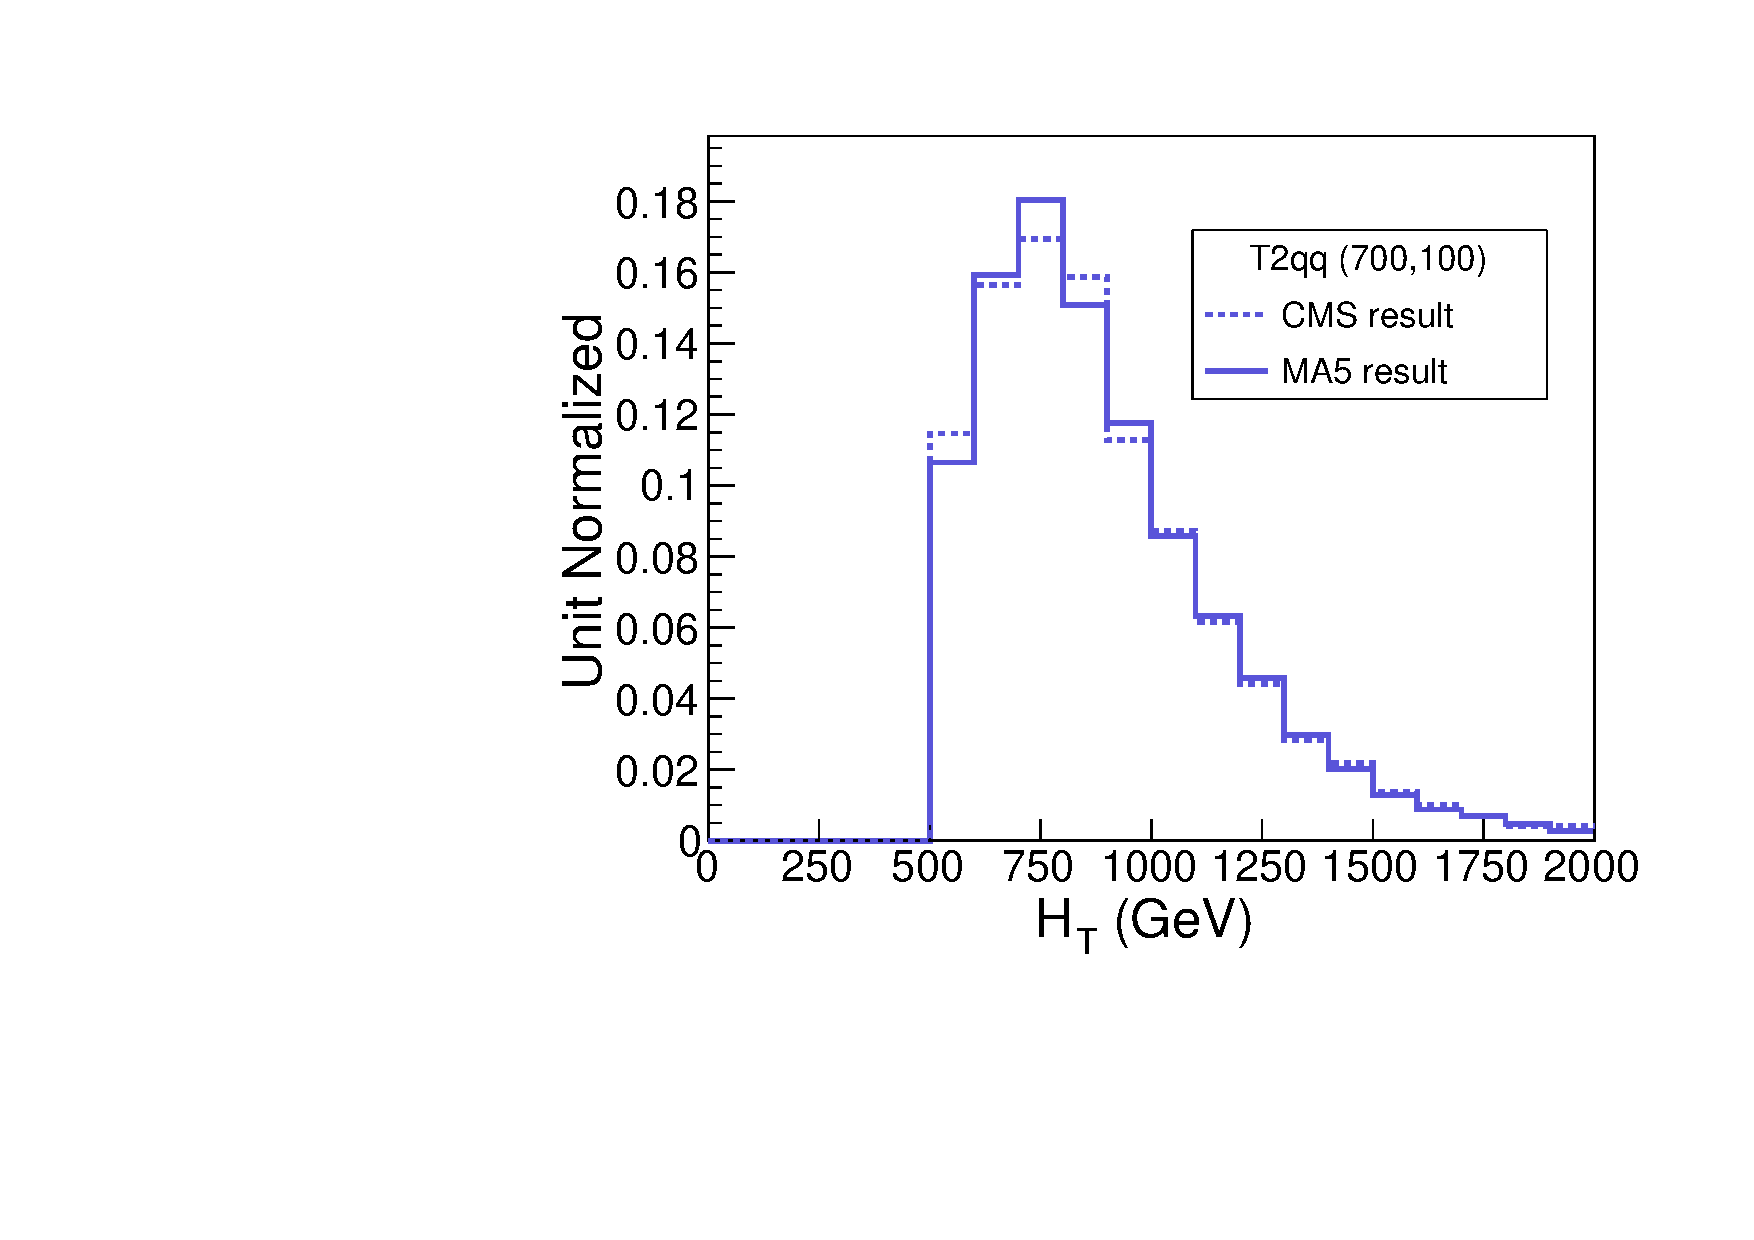
\includegraphics[width=6.4cm]{figures/madanalysis5/cms-012-T2qqHT.pdf}
\caption{Comparison between the official and \ma\ results  for the $\Ht$ distribution after all baseline cuts, 
for the T2qq simplified model of CMS-SUS-13-012 with $(m_{\tilde q},\,m_{\tilde\chi^0_1})=(700,\,100)$~GeV.}
\label{fig:T2qqHT}
\end{figure}

The results of our cut-flow counts for the various simplified models are shown alongside the official counts in 
Tables~\ref{table:CutFlowT1qqqq}  and \ref{table:CutFlowT5VV}. The results 
were obtained by normalizing with the cross section for each 
of the benchmark points and for an integrated luminosity of 19.3~fb$^{-1}$.
Moreover, some distributions after the baseline cuts for the case of the T2qq topology 
are shown in Figs.~\ref{fig:T2qqHT}--\ref{fig:T2qqNJets}. 
The distributions are normalized to unity and overlaid on the official plots obtained from the collaboration.



The agreement between the official and \ma\ results is better than 10\% throughout the baseline cut flows. The largest discrepancy arises from the lepton veto cut, which leads to a difference of up to about 5\% in the cut flow. The shapes of the distributions qualitatively match very well, and the peaking bins are in accordance with the official results. (This also holds for the other distributions not shown here for space considerations). 
The \ma\ implementation is available as \cite{MA5-CMS-SUS-13-012}, and 
a detailed validation note comparing the recast results to those of CMS can be found at \cite{ma5wiki}. 


\begin{figure}
\centering
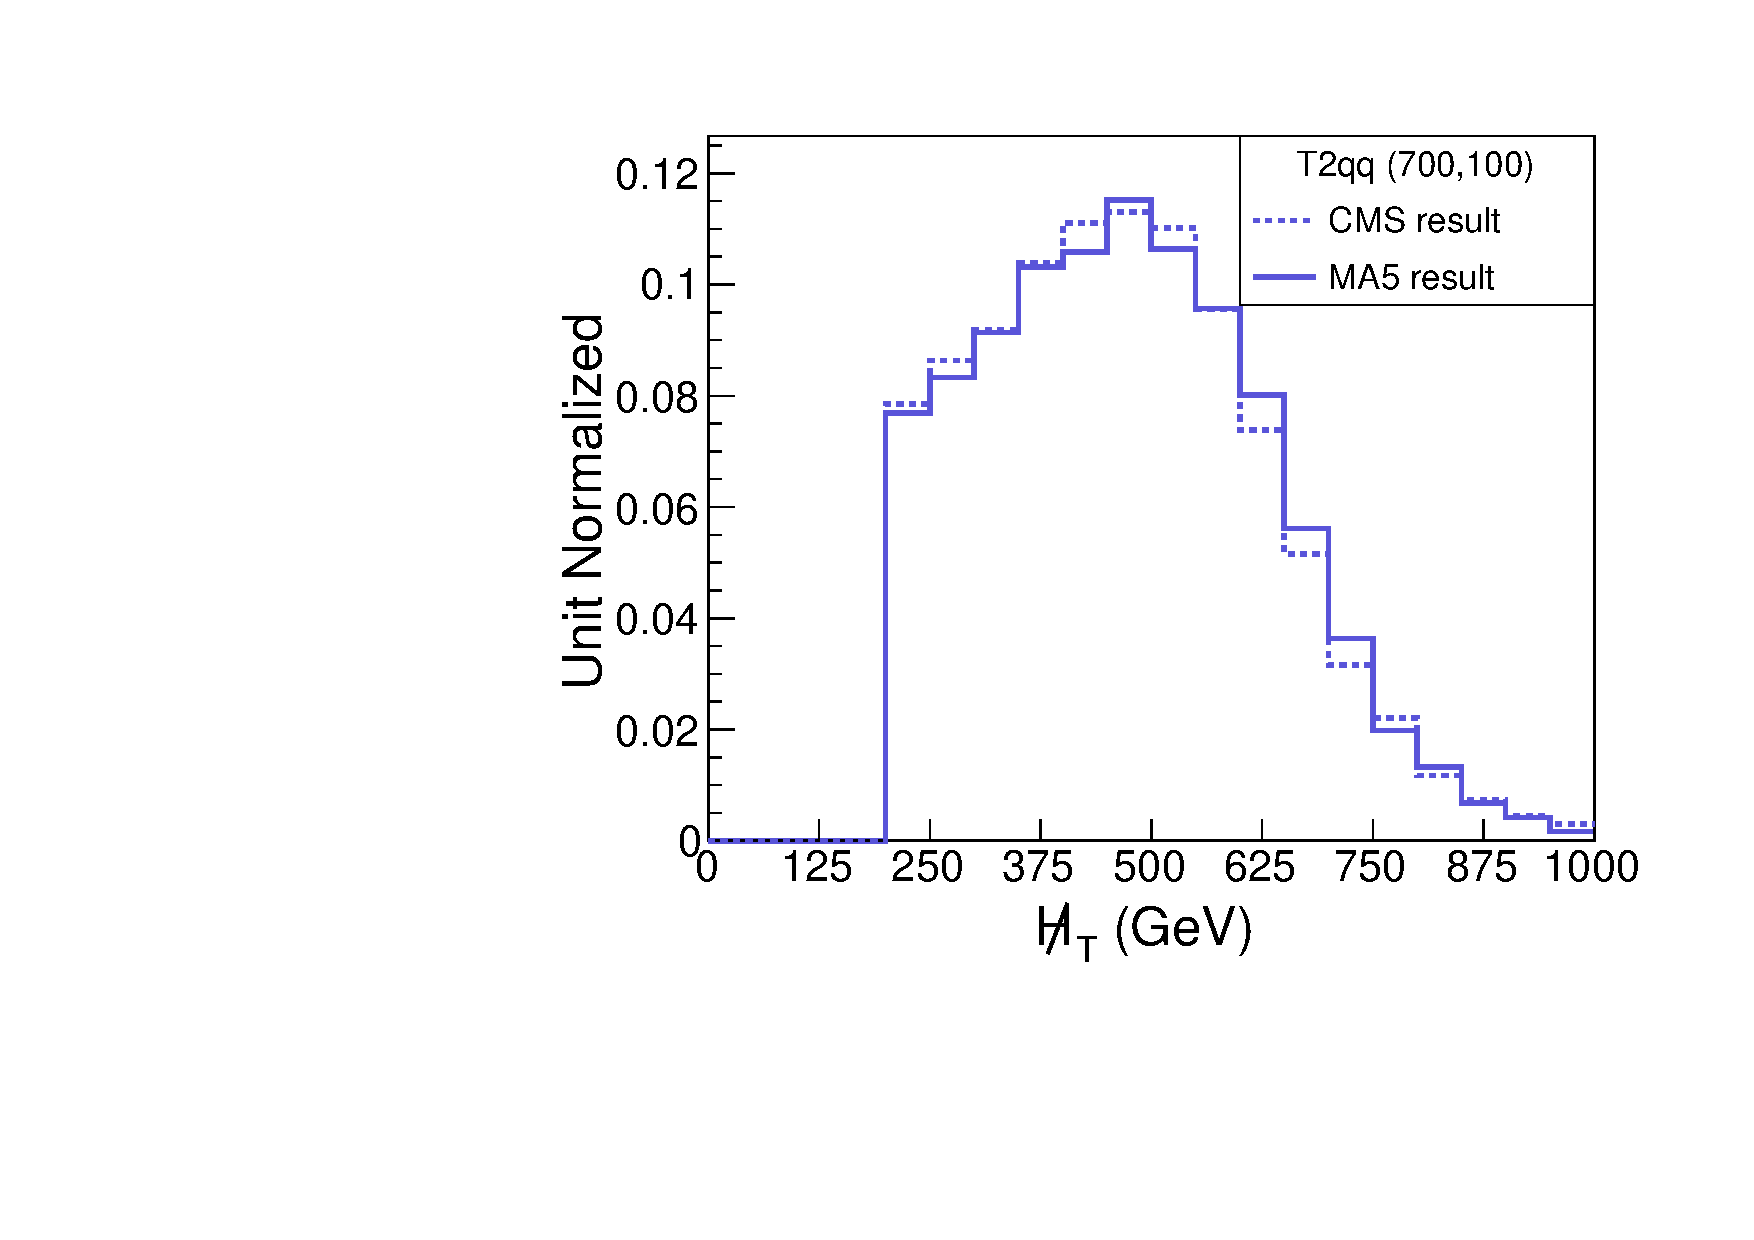
\includegraphics[width=6.4cm]{figures/madanalysis5/cms-012-T2qqMHT.pdf}
\caption{Same as Fig.~\ref{fig:T2qqHT} but for the $\mht$ distribution.}
\label{fig:T2qqMHT}
\end{figure}


\begin{figure}
\centering
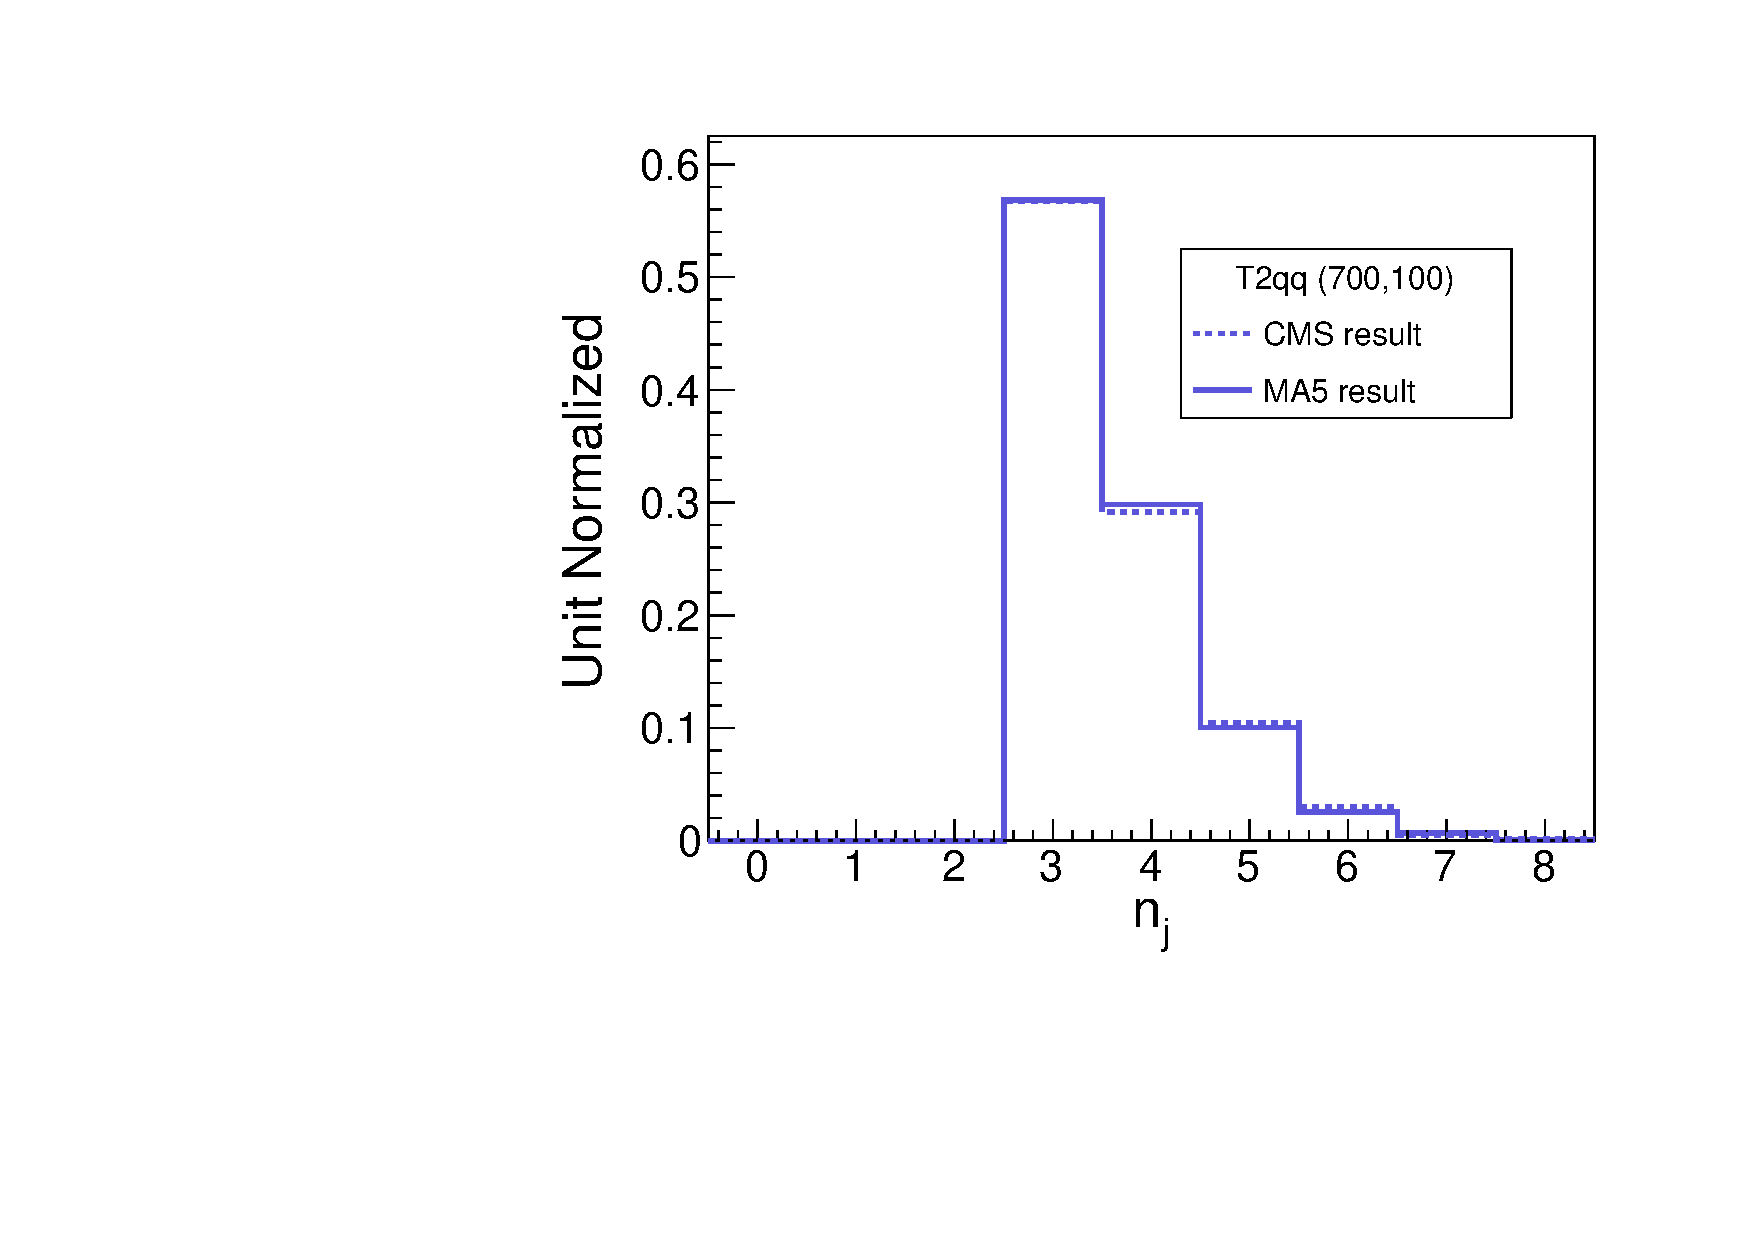
\includegraphics[width=6.4cm]{figures/madanalysis5/cms-012-T2qqNJets.pdf}
\caption{Same as Fig.~\ref{fig:T2qqHT} but for the $\njets$ distribution.}
\label{fig:T2qqNJets}
\end{figure}

%%%%%%%%%%%%%%%%%%%%%%%%%%%%%%%%%%%%%%%%%%%%%%%%%%%%%%%%%

\section{Limit setting}\label{sec:CLprocedure}

%%%%%%%%%%%%%%%%%%%%%%%%%%%%%%%%%%%%%%%%%%%%%%%%%%%%%%%%%


For the statistical interpretation of the results, we provide on \cite{ma5wiki} a {\sc Python} script, 
{\tt exclusion\_CLs.py}, for computing exclusion limits using the $\mathrm{CL}_s$ prescription~\cite{bib-cls}.\footnote{The
{\sc Python} code requires {\sc SciPy} libraries to be installed.}
This code can also be installed on a user system by typing in, from the \ma\ interpreter, the command
\begin{verbatim}
  install RecastingTools
\end{verbatim}
which results in the file \texttt{exclusion\_CLs.py} being present at the
root of any working directory created in the expert mode of \ma. 
We refer to~\cite{Conte:2014zja,ma5wiki} for details on the creation of \ma\ working directories.


The core of the calculation works as follows. First, the number of signal events ($n_s$) is obtained as the
product of the luminosity, signal cross section and acceptance $\times$ efficiency for the SR of interest.
Then, the number of observed events ($n_{\rm obs}$) and the nominal number of background
events ($\hat n_b$) and its uncertainty ($\Delta n_b$), are retrieved from an information card stored in the Analyzer directory, provided by the software package.
A large number of toy MC experiments ($10^5$ by default) are then generated from the Poisson distribution
${\rm poiss}(n_{\rm obs} | n_{\rm expected})$, 
corresponding to the distribution of the total number of events in the SR under the
background-only hypothesis on the one hand ($n_{\rm expected} = n_b$), and under the
signal $+$ background hypothesis ($n_{\rm expected} = n_s + n_b$) on the other hand.
We assume that the uncertainty on the number of background events is modeled as ${\rm gauss}(\hat n_b, \Delta n_b)$,
and for each toy MC the number of background events $n_b$ is randomly generated from this normal distribution.
Under the two different hypotheses, $p$-values are then calculated using the number of events actually observed at the LHC, and finally used to compute the CL$_s$ value.

We have tested the limit-setting code on the analyses presented in this paper and generally found good agreement with the official exclusions from ATLAS and CMS.
As an illustrative example, Fig.~\ref{fig:cms-016-limit} shows the 95\%~CL exclusion limit in the neutralino versus gluino mass plane reproduced with the \ma\ implementation \cite{MA5-CMS-SUS-13-016}  of CMS-SUS-13-016.  

\begin{figure}[!h]\centering
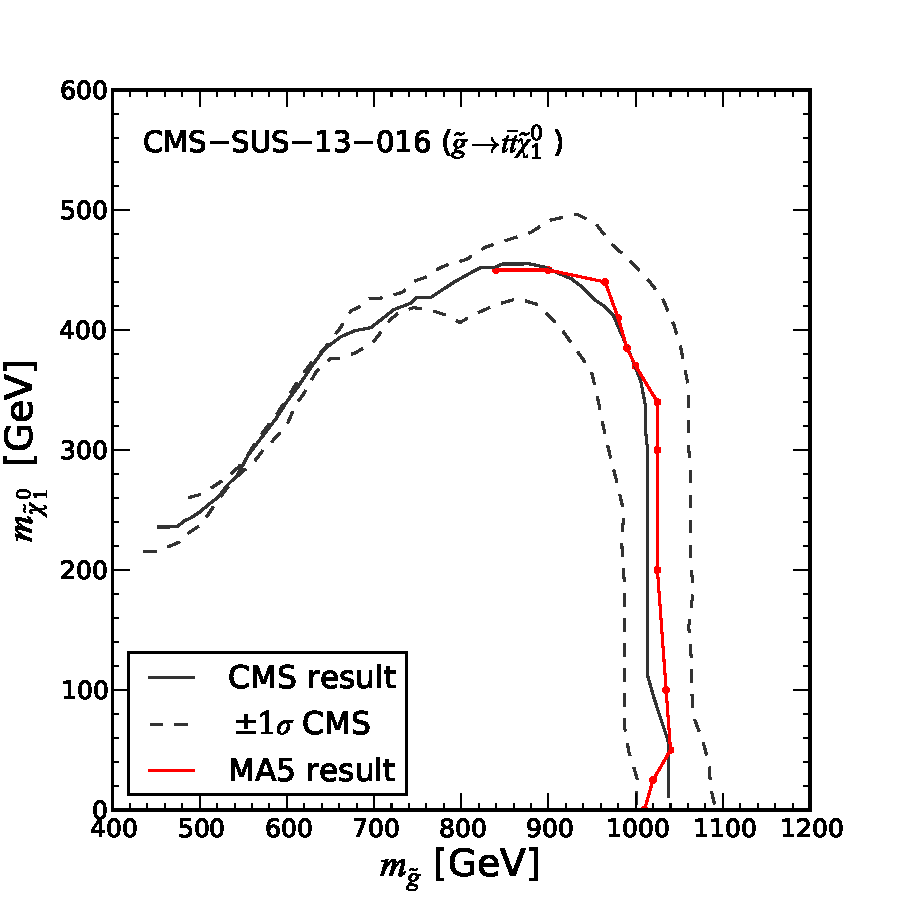
\includegraphics[width=6cm]{figures/madanalysis5/cms-016-limit.pdf}
\caption{The 95\%~CL exclusion limit (in red) in the $\tilde\chi^0_1$ versus $\tilde g$ mass plane reproduced 
with the \ma\ implementation  \cite{MA5-CMS-SUS-13-016}  of CMS-SUS-13-016. For comparison, the full and dashed grey lines show the official CMS result with its $\pm1\sigma$ uncertainty from Fig.~6 of \cite{CMS:2013ija}. 
The limit setting in the region where one of the tops from the gluino decay is off-shell, \ie\ for $m_{\tilde g}\lesssim 800$~GeV, is work in progress.} 
\label{fig:cms-016-limit}
\end{figure}


%%%%%%%%%%%%%%%%%%%%%%%%%%%%%%%%%%%%%%%%%%%%%%%%%%%%%%%%%

\section{\ma\ conclusions}\label{sec:conclusions}

%%%%%%%%%%%%%%%%%%%%%%%%%%%%%%%%%%%%%%%%%%%%%%%%%%%%%%%%%

We have presented a new scheme for developing and deploying implementations of LHC analyses 
based on fast simulation within the \ma\ framework. This can serve to create a public analysis database,  
which may be used and developed further by the whole community.  
The code for the five analyses~\cite{MA5-CMS-SUS-13-011,MA5-CMS-SUS-13-012,MA5-CMS-SUS-13-016,MA5-ATLAS-SUSY-2013-05,MA5-ATLAS-SUSY-2013-11} 
that we published together with this paper are intended as a starting point 
for this database and may conveniently be used as templates for other analyses.  

We propose that the C++ code of new implementations within this scheme be published 
via {\sc Inspire}~\cite{inspire}, as done here,  
best together with the physics paper they have been developed for. 
This way, each analysis implementation is assigned a 
Digital Object Identifier (DOI)~\cite{doi}, ensuring that it is uniquely identifiable, searchable and citable. 
In addition it is very useful if a detailed validation note is made available on the  \ma\ wiki page~\cite{ma5wiki}. 

The ease with which an experimental analysis can be implemented and validated may serve as a useful check for the experimental collaborations for the quality of their documentation. Note, finally, that the platform we are pro\-posing might also be used by the experimental collaborations to directly provide implementations of their analyses for fast simulation, thereby assuring the maximum usability of their results, as for example envisaged in level 1 of the CMS statement on ``data preservation, re-use and open access policy'' \cite{CMS:DataPolicy}. 

The author of a re-implementation could be a new member of CMS or ATLAS who wishes to learn about an analysis, or a who has recently carried out an analysis and wants the analysis to have a larger impact. Such a volunteer must read the relevant CMS paper and implement the object and event selection in a relatively easy-to-use framework based on c++, and validate their implementation by comparing their results for cut flows and exclusion limit curves with those that CMS makes public. Sample validation material has been given above, and examples of complete validation documents are provided in Sections~\ref{app:ma5multijet} and \ref{app:ma5stop}.

It is important for the legacy of the LHC that its experimental results can be used by the whole high-energy physics community. We hope that our project contributes to this aim. 

\section{Implementation of (SUS-13-012)}
\label{app:ma5multijet}
The following describes the work documented in \cite{MA5-CMS-SUS-13-012}, in association with the paper~\cite{MA5-CMS-SUS-13-012}.
%%%%%%%%%%%%%%%%%%%%%%%%%%%%%%%%%%%%%%%%%%%%%%%%%
\textbf{Bein, Samuel (Florida State U.); Sengupta, Dipan (LPSC, Grenoble)}\\
We present the results of the synchronization of the MA5
implementation of the SUS-13-012 multi-jet $+$ $\mht$ SUSY search for SUSY in data collected 
by the CMS experiment at $\sqrt{s}=$ 8 TeV.  The
performance of the implementation is evaluated by comparing the
MA5-derived results with a set of cut flow tables and kinematic
distributions provided by CMS for this purpose. The simplified models
T1qqqq (Figure \ref{fig:T1qqqq}), T1tttt (Figure \ref{fig:T1tttt}), T5VV (Figure \ref{fig:T5VV}), and T2qq (Figure \ref{fig:T2qq}), are used as common benchmarks, with values of the masses of the
gluino and neutralino taking on a range of values. Two types of
comparisons are given in Figs. \ref{table:CF1}$-$\ref{fig:last} give cut flow tables and normalized
kinematic distributions. In some cases the
cut flow tables give the number of events normalized to 100\%; in
other cases the tables are normalized to the cross section times the
integrated luminosity. The normalization convention used by CMS was
followed. Dashes hold the place of values that were not
provided in the CMS cut flow tables. 

\subsection{T1qqqq simplified model}
\begin{figure}[h!]
\centering
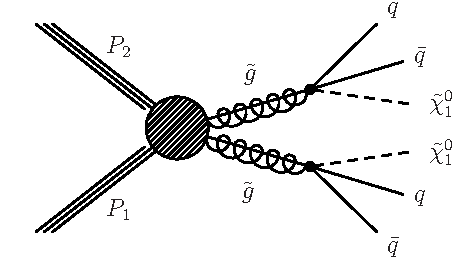
\includegraphics[width=7cm]{figures/Appendices/Ma5ValidationSUS13012/T1qqqq.pdf}
\caption{Diagram of the dominant SUSY production mechanism
for the T1qqqq signal model.}
\label{fig:T1qqqq}
\end{figure}

    \begin{table}[h!]
    \begin{centering}
    \begin{tabular}{  c | c | c  }
    \hline
    \hline	
    Cut Name & Official Count (Eff) & MA5 Count (Eff)\\
    \hline
        MET Cleaning & 190.6 (xxx) & 190.6 (xxx)\\
    No Lepton & 190.3 (99\%) & 190.6 (100\%)\\
    NJets$>$2 & 188.1 (98\%) & 188.49 (98\%)\\
    $H_T$$>$500 & 187.6 (99\%) & 188.07 (99\%)\\
    \MHT$>$200 & 158.7 (84\%) & 159.72 (84\%)\\
    Min $\Delta(\phi)$ & 130.8 (82\%) & 131.11 (82\%)\\
\hline
\hline
    \end{tabular}
    \caption{The cut flow for the baseline selection in CMS SUS-13-012 for
    the  T1qqqq working point $(m_{\tilde g},\,m_{\tilde\chi^0_1})=(1100,\,125)$~GeV. 
    The second column is the official account as
    reported by 
    https://twiki.cern.ch/twiki/pub/CMSPublic/PhysicsResultsSUS13012/T1qqqq.pdf,
    and our own results are given in column 3. The official counts are
    normalized to luminosity ${\cal L}=19.5$/fb and cross section $\sigma= 10.17$~pb, and our
    counts are normalized to match the official count after the first cut, MET
    Cleaning.}
    \label{table:CF1}
    \end{centering}
    \end{table}
    
    \begin{table}
    \begin{centering}
    \begin{tabular}{  l | c | c  }
    \hline
    \hline
    Signal Region Name & Official & MA5\\
    \hline
    NJets3-5,  $H_T$500-800,  \MHT200-300 & 1.4 & 1.21\\ 
 \hline 
NJets3-5,  $H_T$500-800,  \MHT300-450 & 2.4 & 2.08\\ 
 \hline 
NJets3-5,  $H_T$500-800,  \MHT450-600 & 1.7 & 1.36\\ 
 \hline 
NJets3-5,  $H_T$500-800,  \MHT$>$600 & 0.6 & 0.60\\ 
 \hline 
NJets3-5,  $H_T$800-1000,  \MHT200-300 & 2.1 & 1.81\\ 
 \hline 
NJets3-5,  $H_T$800-1000,  \MHT300-450 & 2.9 & 3.75\\ 
 \hline 
NJets3-5,  $H_T$800-1000,  \MHT450-600 & 4.2 & 3.74\\ 
 \hline 
NJets3-5,  $H_T$800-1000,  \MHT$>$600 & 4.1 & 4.04\\ 
 \hline 
NJets3-5,  $H_T$1000-1250,  \MHT200-300 & 4.2 & 3.70\\ 
 \hline 
NJets3-5,  $H_T$1000-1250,  \MHT300-450 & 8.1 & 6.93\\ 
 \hline 
NJets3-5,  $H_T$1000-1250,  \MHT450-600 & 7.6 & 7.18\\ 
 \hline 
NJets3-5,  $H_T$1000-1250,  \MHT$>$600 & 10.6 & 10.63\\ 
 \hline 
NJets3-5,  $H_T$1250-1500,  \MHT200-300 & 3.9 & 3.64\\ 
 \hline 
NJets3-5,  $H_T$1250-1500,  \MHT300-450 & 7.3 & 6.74\\ 
 \hline 
NJets3-5,  $H_T$1250-1500,  \MHT$>$450 & 15.6 & 16.52\\ 
 \hline 
NJets3-5,  $H_T$$>$1500,  \MHT200-300 & 4.5 & 4.41\\ 
 \hline 
NJets3-5,  $H_T$$>$1500,  \MHT$>$300 & 17.9 & 18.80\\ 
 \hline 
NJets6-7,  $H_T$500-800,  \MHT200-300 & 0.1 & 0.08\\ 
 \hline 
NJets6-7,  $H_T$500-800,  \MHT300-450 & 0.1 & 0.05\\ 
 \hline 
NJets6-7,  $H_T$500-800,  \MHT$>$450 & 0.1 & 0.04\\ 
 \hline 
NJets6-7,  $H_T$800-1000,  \MHT200-300 & 0.3 & 0.24\\ 
 \hline 
NJets6-7,  $H_T$800-1000,  \MHT300-450 & 0.6 & 0.51\\ 
 \hline 
NJets6-7,  $H_T$800-1000,  \MHT$>$450 & 0.8 & 0.71\\ 
 \hline 
NJets6-7,  $H_T$1000-1250,  \MHT200-300 & 0.9 & 0.91\\ 
 \hline 
NJets6-7,  $H_T$1000-1250,  \MHT300-450 & 1.8 & 1.74\\ 
 \hline 
NJets6-7,  $H_T$1000-1250,  \MHT$>$450 & 2.8 & 2.94\\ 
 \hline 
NJets6-7,  $H_T$1250-1500,  \MHT200-300 & 1.2 & 1.16\\ 
 \hline 
NJets6-7,  $H_T$1250-1500,  \MHT300-450 & 2.4 & 2.46\\ 
 \hline 
NJets6-7,  $H_T$1250-1500,  \MHT$>$450 & 4.1 & 5.16\\ 
 \hline 
NJets6-7,  $H_T$$>$1500,  \MHT200-300 & 2.3 & 2.56\\ 
 \hline 
NJets6-7,  $H_T$$>$1500,  \MHT$>$300 & 9.8 & 11.50\\ 
 \hline 
NJets$>$7,  $H_T$500-800,  \MHT$>$200 & 0.0 & 0.0\\ 
 \hline 
NJets$>$7,  $H_T$800-1000,  \MHT$>$200 & 0.0 & 0.01\\ 
 \hline 
NJets$>$7,  $H_T$1000-1250,  \MHT$>$200 & 0.2 & 0.28\\ 
 \hline 
NJets$>$7,  $H_T$1250-1500,  \MHT$>$200 & 0.5 & 0.75\\ 
 \hline 
NJets$>$7,  $H_T$$>$1500,  \MHT$>$200 & 2.2 & 2.69\\ 
 \hline 
\hline
    \end{tabular}
    \caption{The signal region (SR) counts in CMS SUS-13-012 for the T1qqqq scenario 
    after all selection has been applied. Column 2 is the official account obtained through generous correspondence with Christian Sanders,
    and our own results displayed in column 3. These counts were determined by applying the SR selection to the end of the cut flow featured in table \ref{table:CF1}.}
    \label{table:CF2}
    \end{centering}
    \end{table}
    
\begin{figure}
        \centering
        \subfloat[]{
                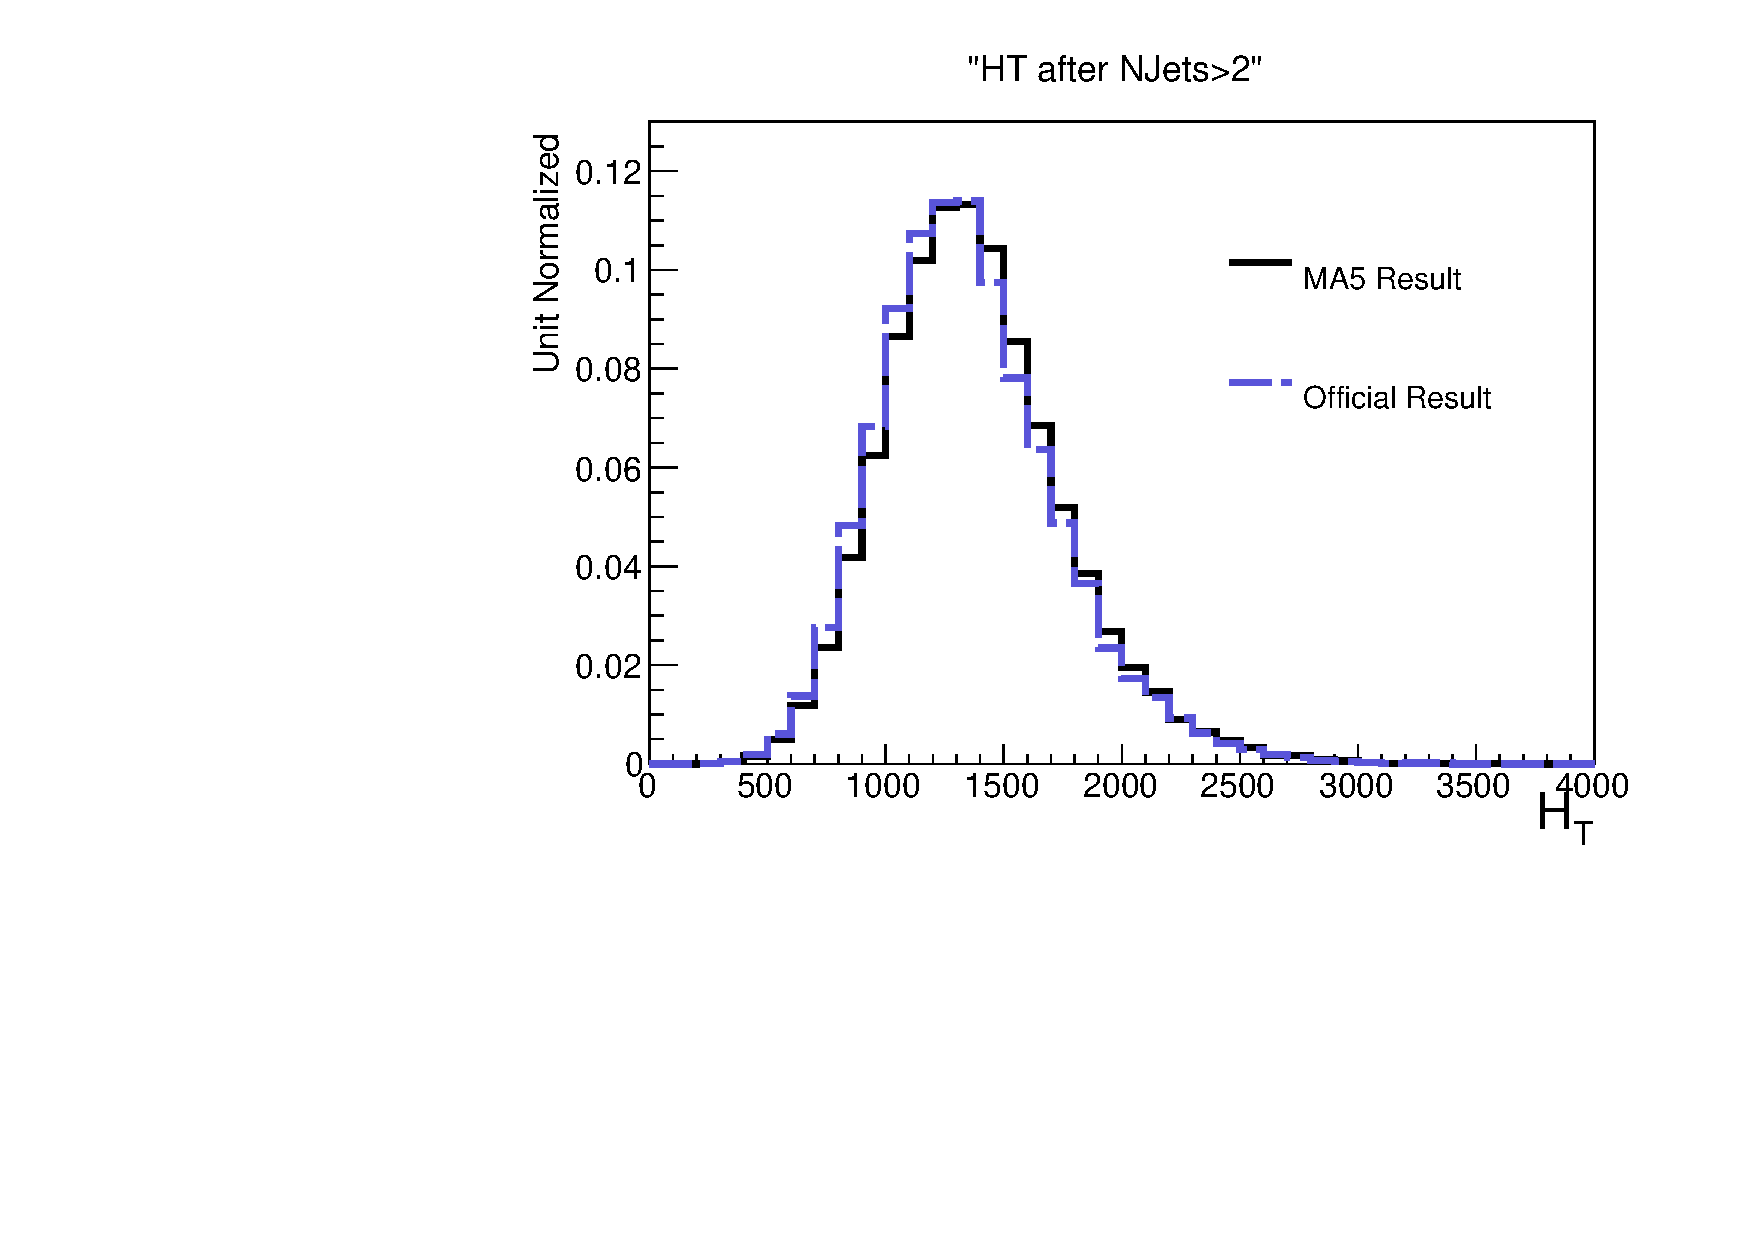
\includegraphics[width=0.5\textwidth]{figures/Appendices/Ma5ValidationSUS13012/T1qqqq_HT_after_NJets>2.pdf}
                \label{fig:gull}
        }%
        \hspace{-1 cm}
        ~ %add desired spacing between images, e. g. ~, \quad, \qquad, \hfill etc.
          %(or a blank line to force the subfigure onto a new line)
        \subfloat[]{
                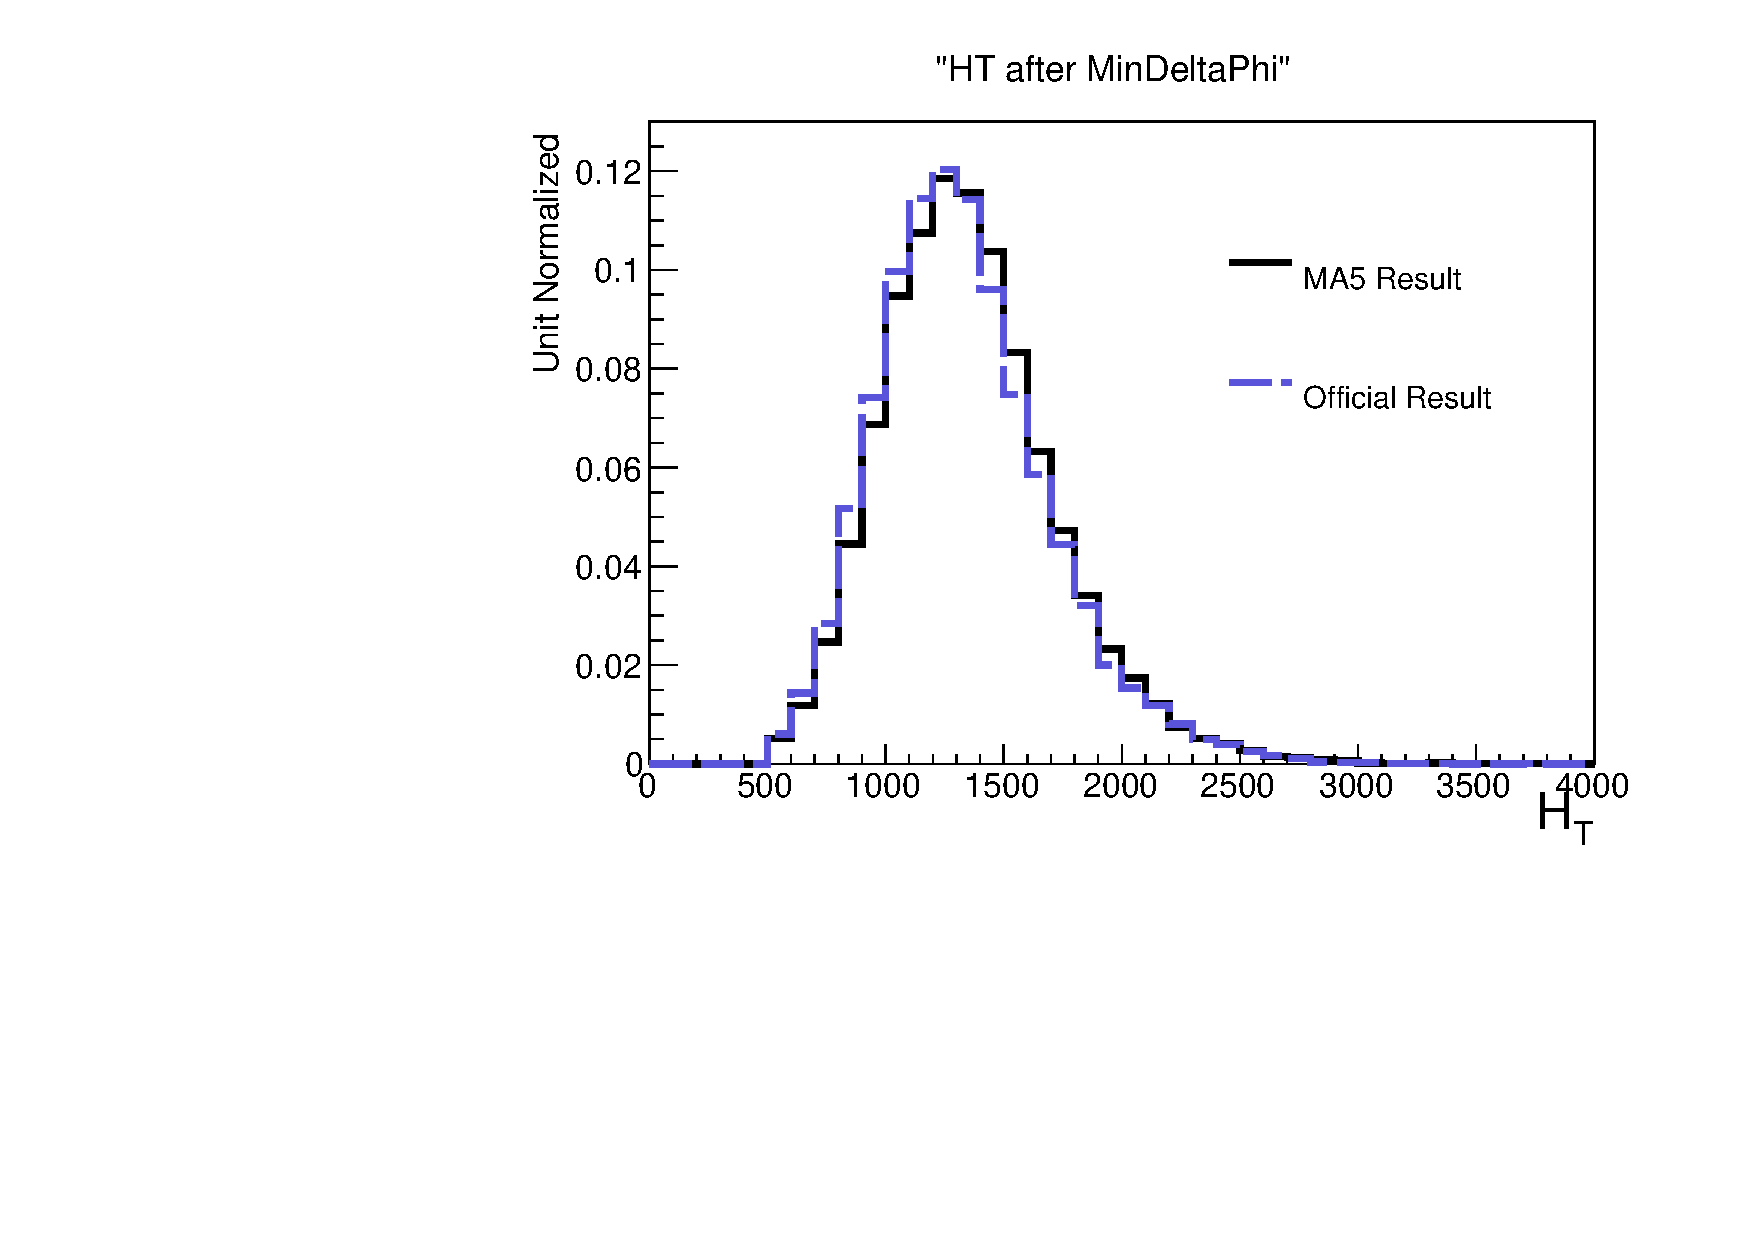
\includegraphics[width=0.5\textwidth]{figures/Appendices/Ma5ValidationSUS13012/T1qqqq_HT_after_MinDeltaPhi.pdf}
                \label{fig:tiger}
        }
        \caption{Comparison of the distributions of $H_T$ between the official and our own samples after the ``n-1" cut, Min $\Delta(\phi)$ (left), and after all baseline cuts (right), for the T1qqqq signal model.}\label{fig:animals}
\end{figure}        
        
\begin{figure}
        \centering
        \subfloat[]{
                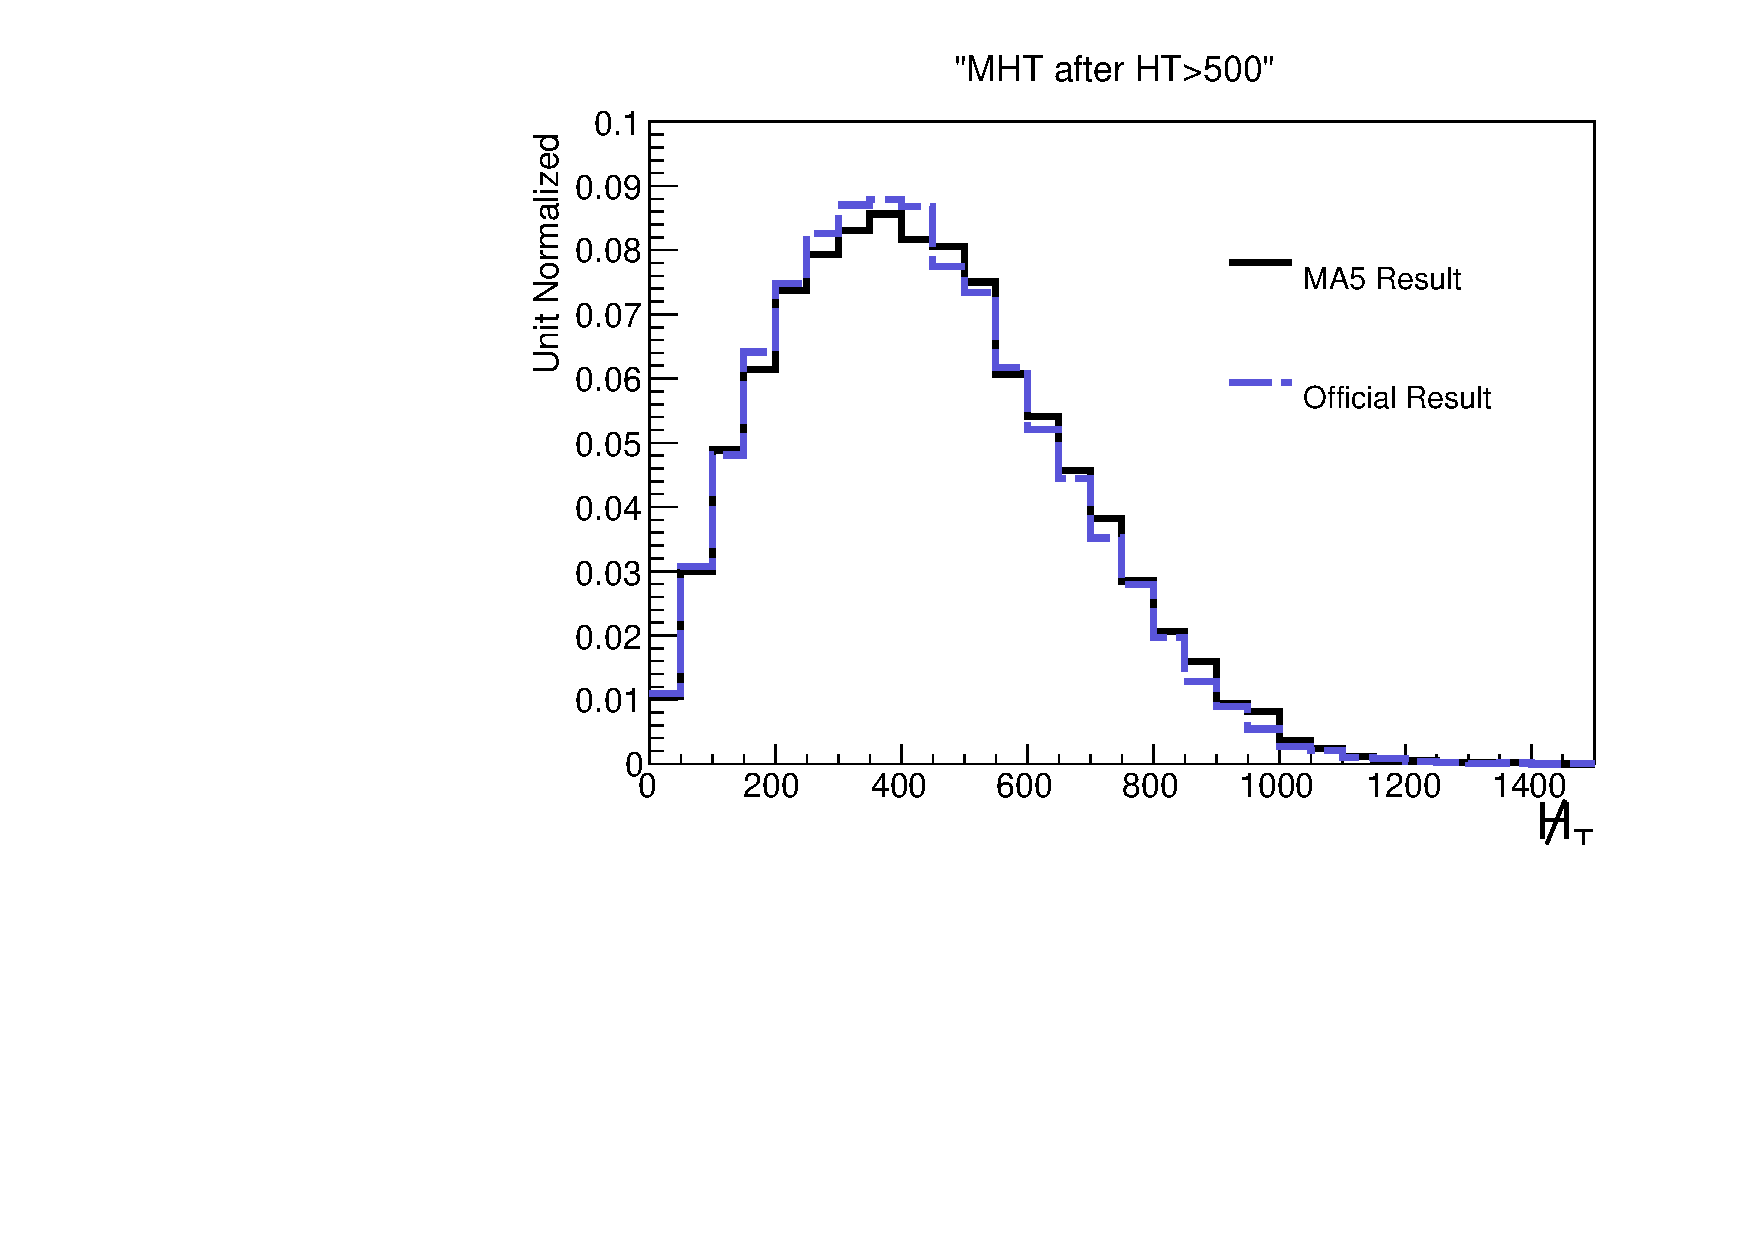
\includegraphics[width=0.5\textwidth]{figures/Appendices/Ma5ValidationSUS13012/T1qqqq_MHT_after_HT>500.pdf}
                \label{fig:gull}
        }%
        \hspace{-1 cm}
        ~ %add desired spacing between images, e. g. ~, \quad, \qquad, \hfill etc.
          %(or a blank line to force the subfigure onto a new line)
        \subfloat[]{
                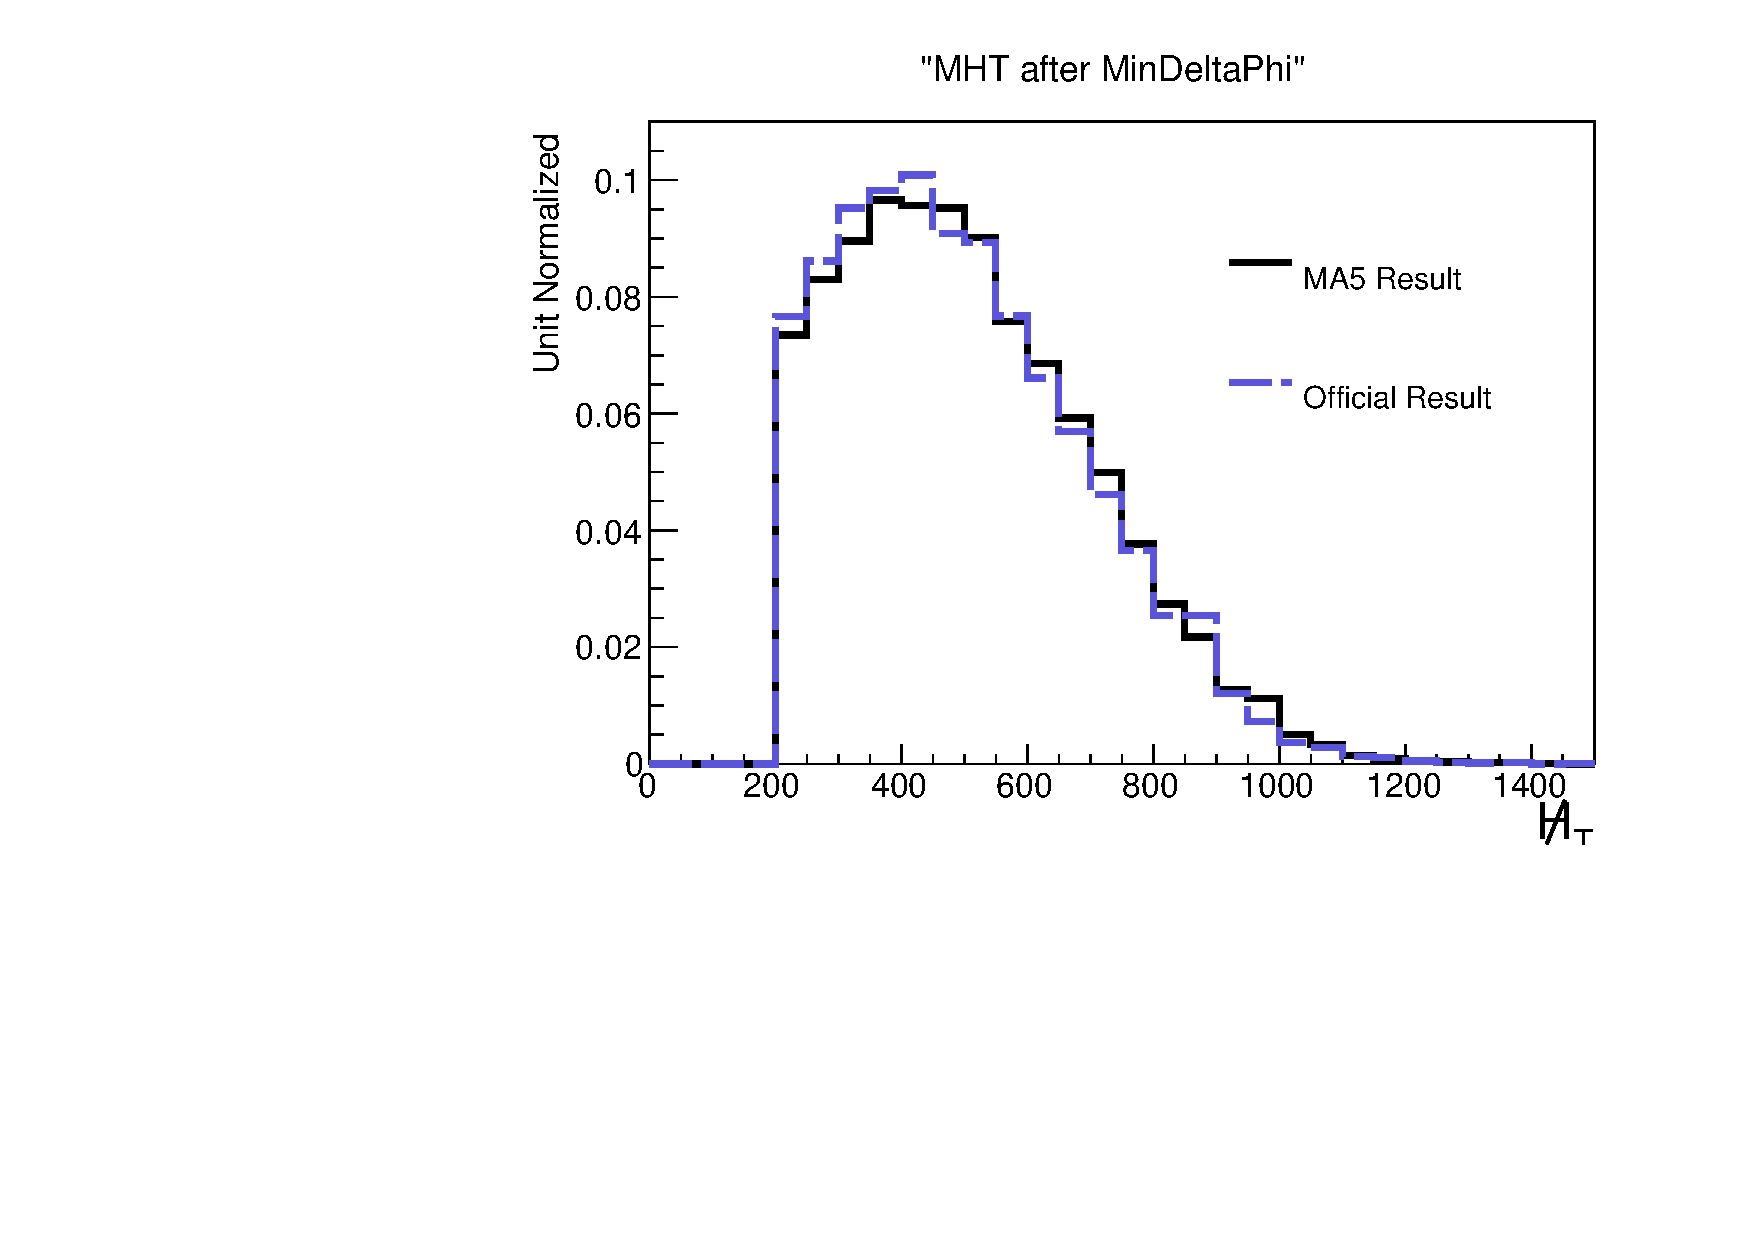
\includegraphics[width=0.5\textwidth]{figures/Appendices/Ma5ValidationSUS13012/T1qqqq_MHT_after_MinDeltaPhi.pdf}
                \label{fig:tiger}
        }
        \caption{Comparison of the distributions of \MHT between the official and our own samples after the ``n-1" cut, Min $\Delta(\phi)$ (left), and after all baseline cuts (right), for the T1qqqq signal model.}\label{fig:animals}
\end{figure}        
        
\begin{figure}
        \centering
        \subfloat[]{
                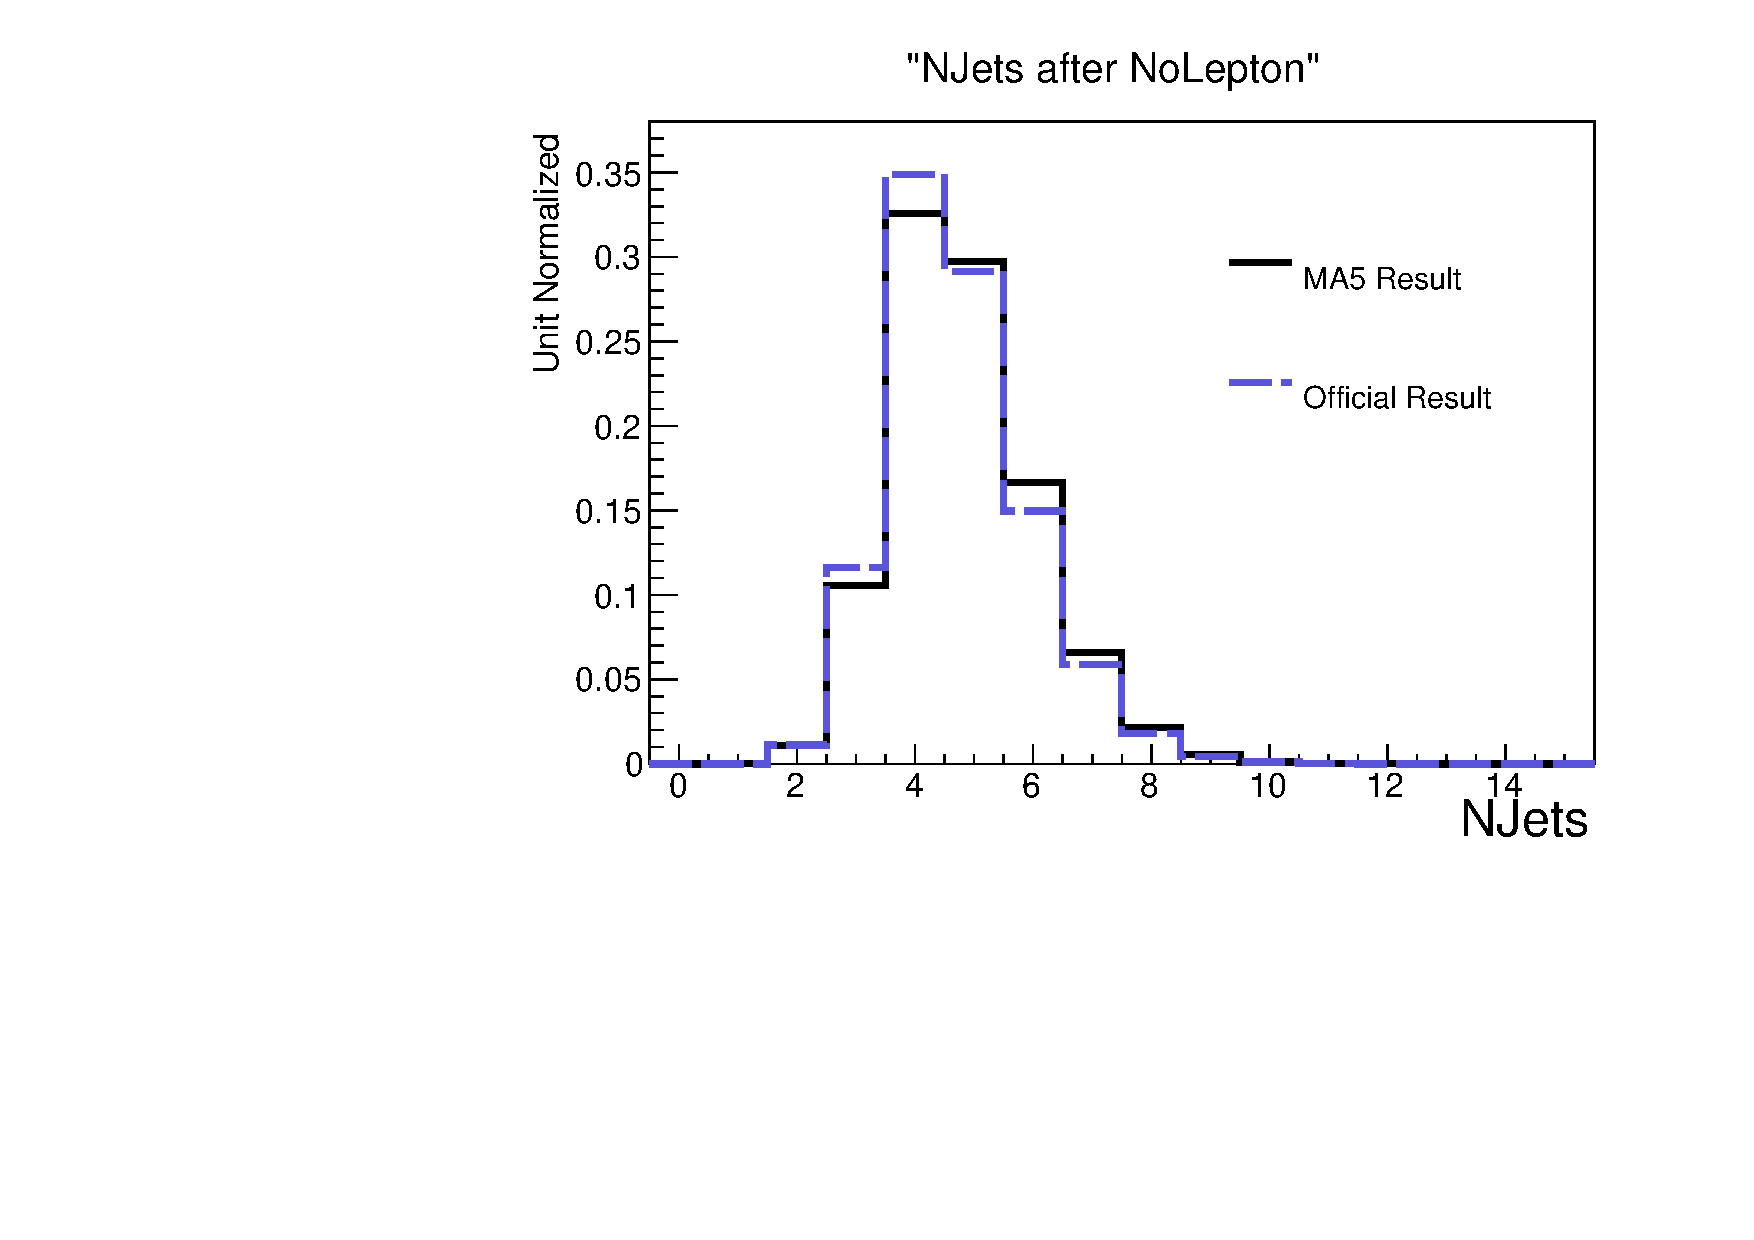
\includegraphics[width=0.5\textwidth]{figures/Appendices/Ma5ValidationSUS13012/T1qqqq_NJets_after_NoLepton.pdf}
                \label{fig:gull}
        }%
        \hspace{-1 cm}
        ~ %add desired spacing between images, e. g. ~, \quad, \qquad, \hfill etc.
          %(or a blank line to force the subfigure onto a new line)
        \subfloat[]{
                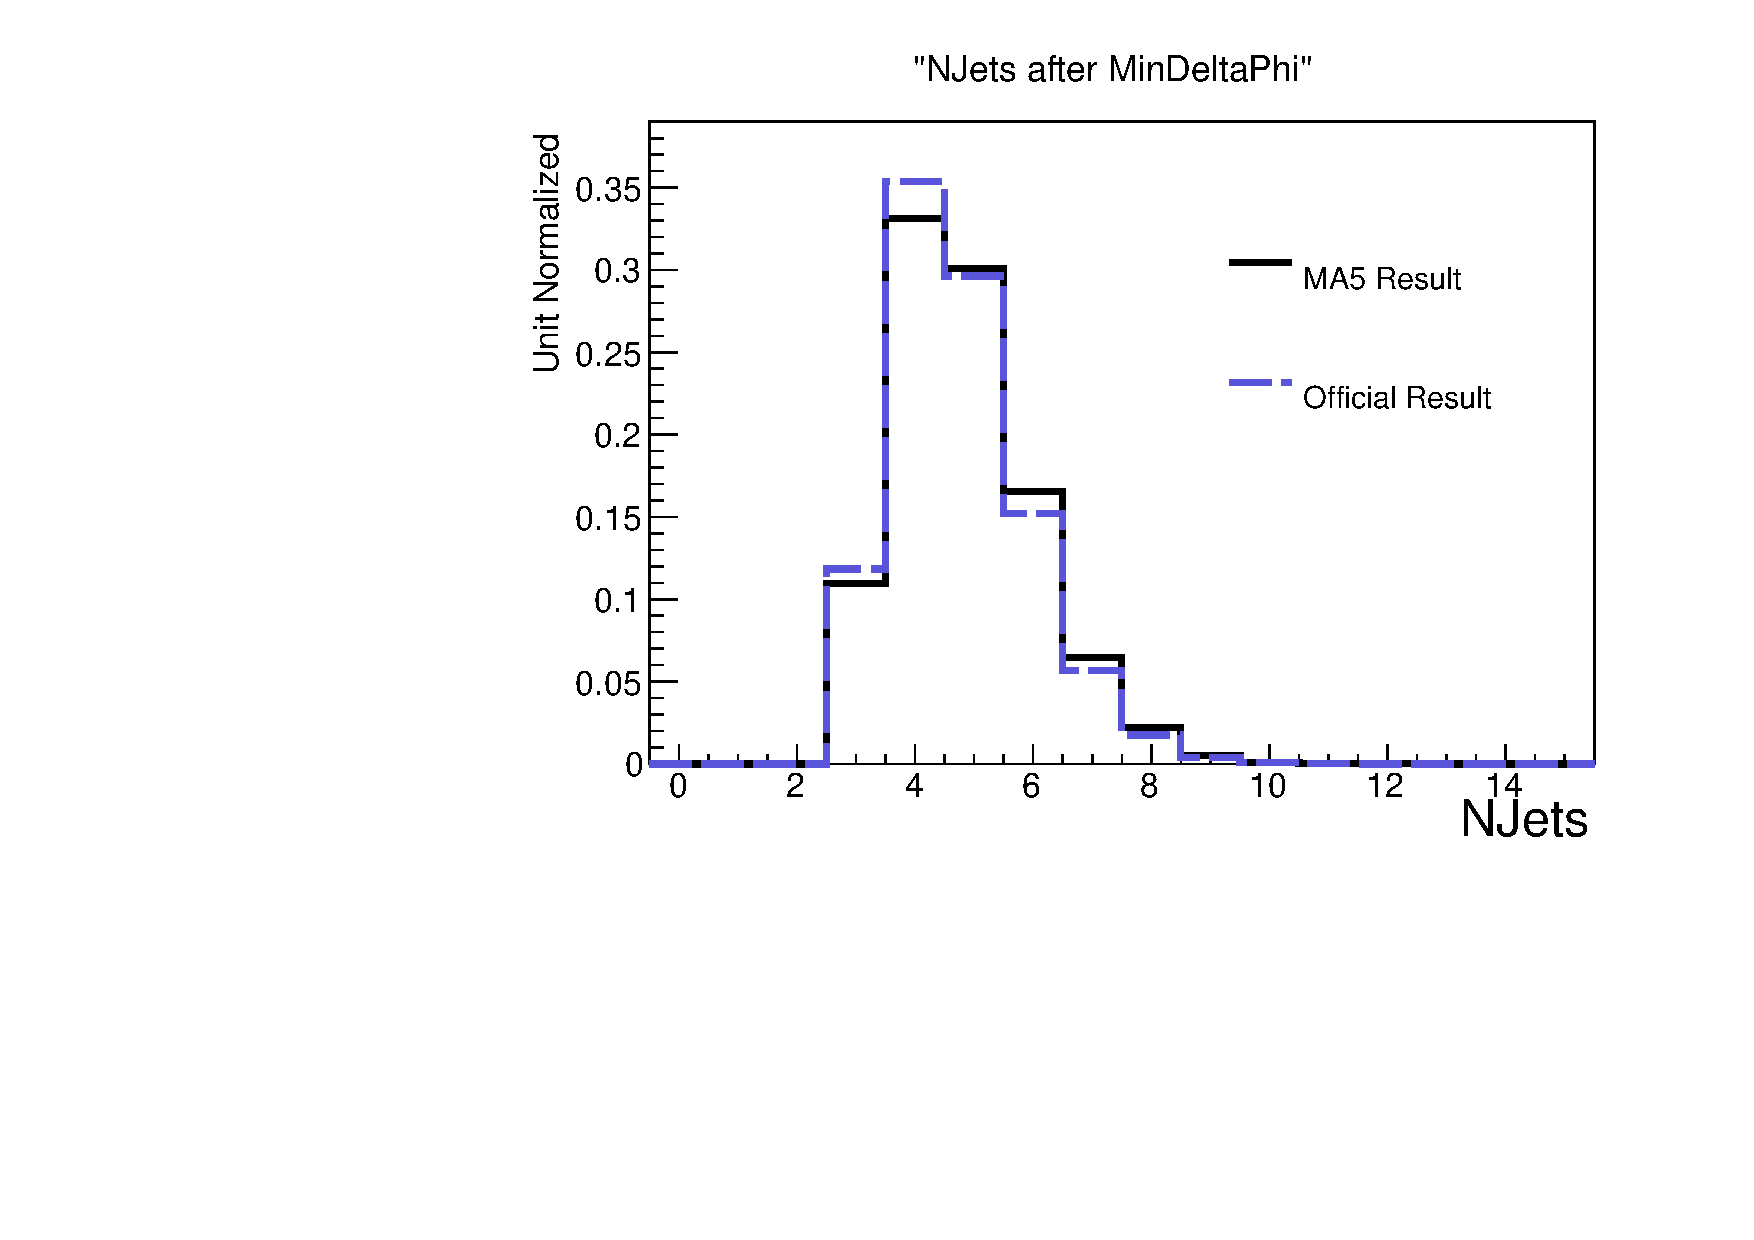
\includegraphics[width=0.5\textwidth]{figures/Appendices/Ma5ValidationSUS13012/T1qqqq_NJets_after_MinDeltaPhi.pdf}
                \label{fig:tiger}
        }
        \caption{Comparison of the distributions of NJets between the official and our own samples after the ``n-1" cut, Min $\Delta(\phi)$ (left), and after all baseline cuts (right), for the T1qqqq signal model.}\label{fig:animals}
\end{figure}        
        
        \begin{figure}
        \centering
        \subfloat[]{
        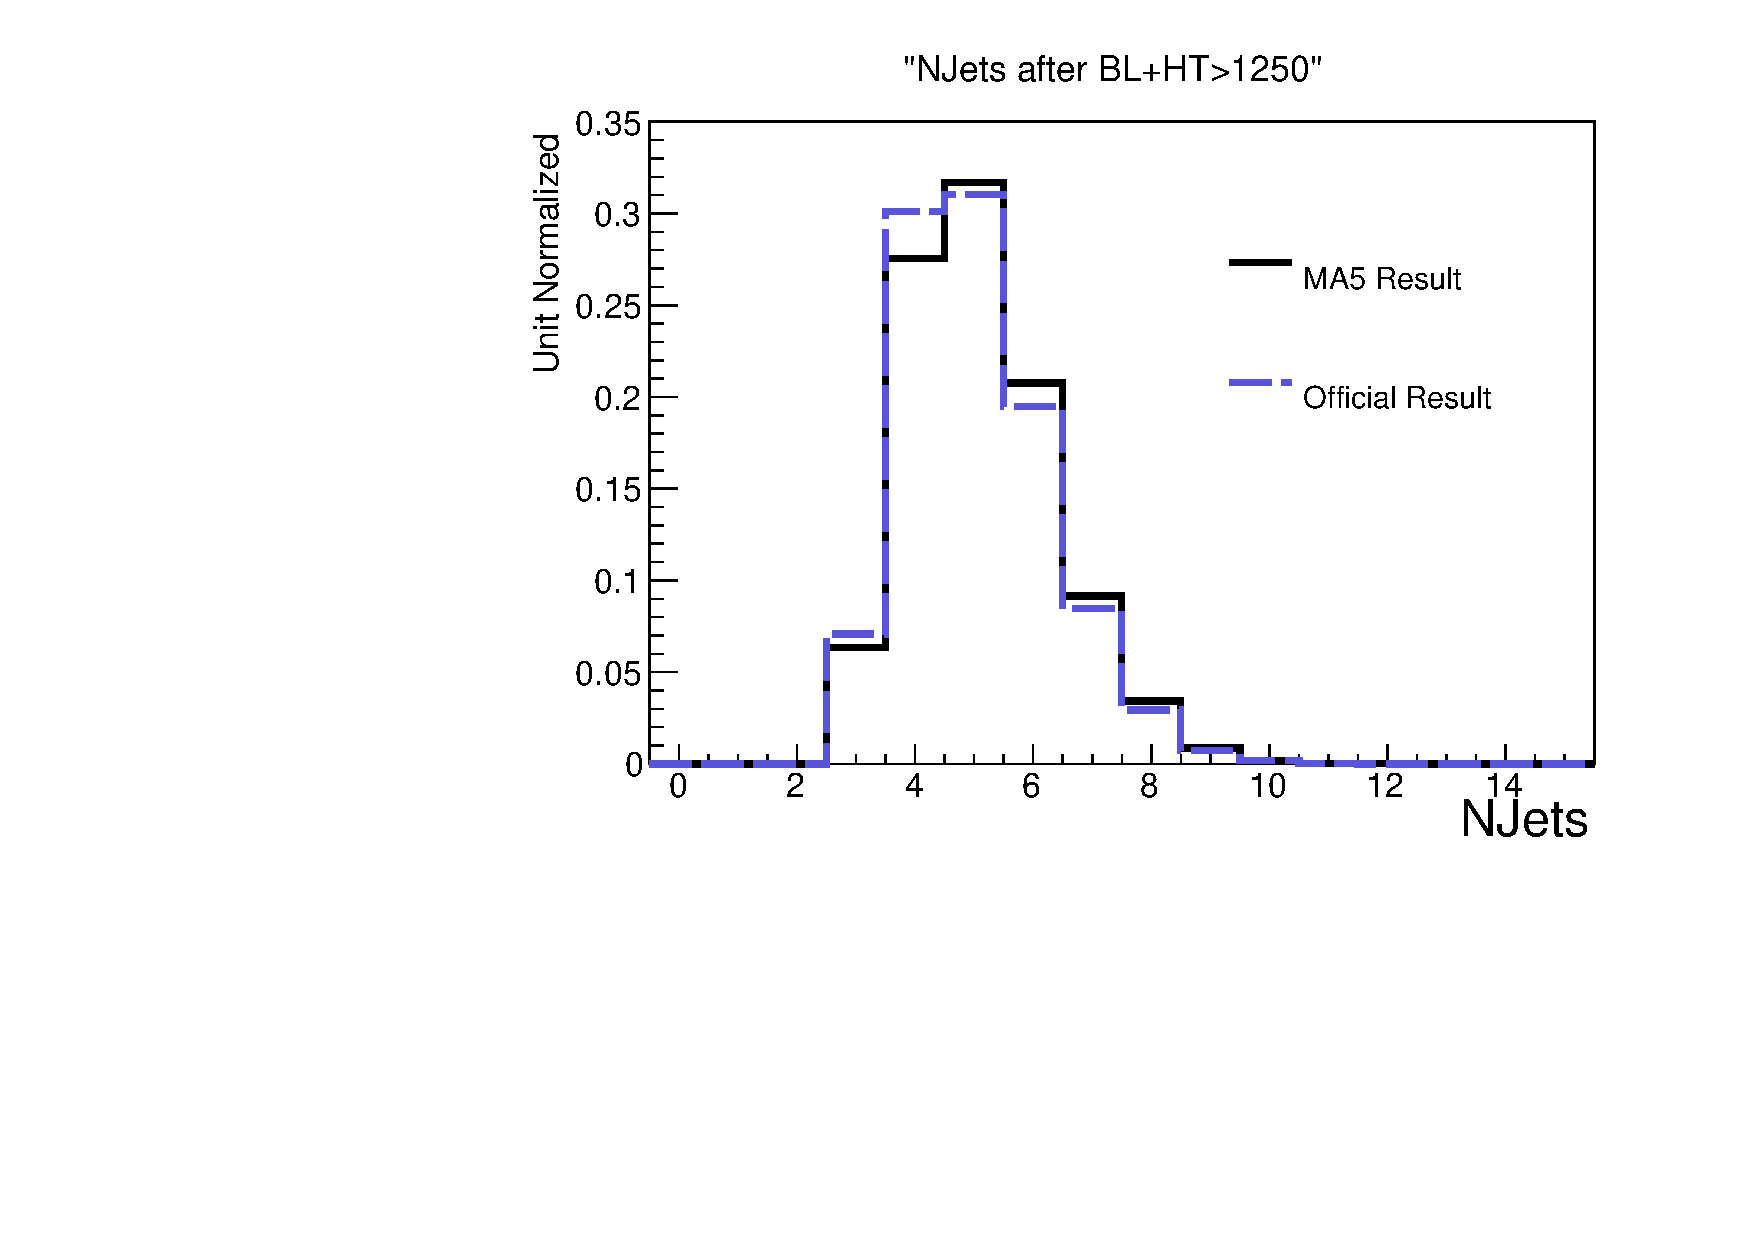
\includegraphics[width=0.5\textwidth]{figures/Appendices/Ma5ValidationSUS13012/T1qqqq_NJets_after_BL+HT>1250.pdf}
        \label{fig:gull}
        }%
        \hspace{-1 cm}
        ~ %add desired spacing between images, e. g. ~, \quad, \qquad, \hfill etc.
        %(or a blank line to force the subfigure onto a new line)
        \subfloat[]{
        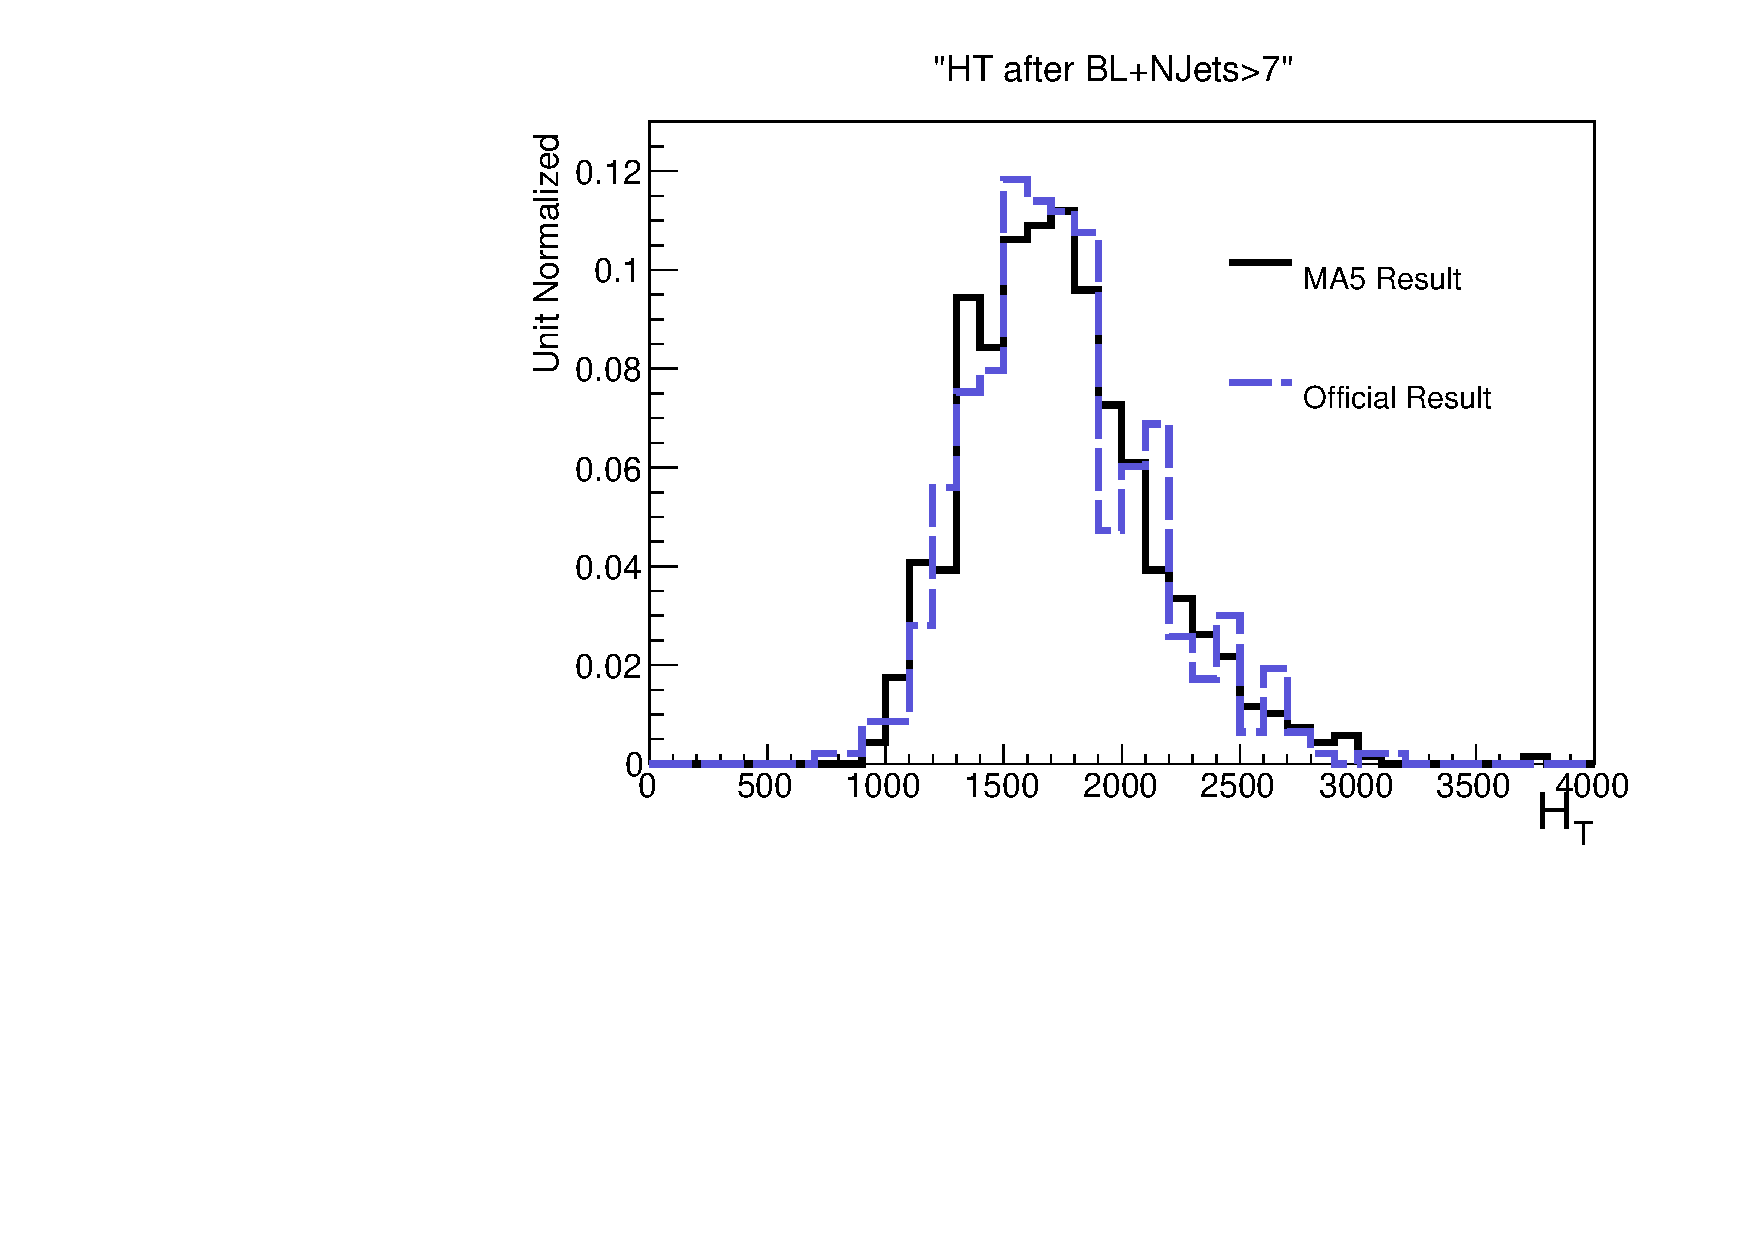
\includegraphics[width=0.5\textwidth]{figures/Appendices/Ma5ValidationSUS13012/T1qqqq_HT_after_BL+NJets>7.pdf}
        \label{fig:tiger}
        }
        \caption{Additional checks: comparison between ours and the official distributions of NJets after BL+$H_T$$>$1250 cuts (left), and $H_T$ after BL+NJets$>$7 cuts (right), for the T1qqqq signal model.}
        \end{figure}        

\clearpage
%%%%%%%%%%%%%%%%%%%%%%%%%%%%%%%%%%%%%%%%%%%%%%%%%
\subsection{T1tttt simplified model}
%%%%%%%%%%%%%%%%%%%%%%%%%%%%%%%%%%%%%%%%%%%%%%%%%

\begin{figure}[h!]
\centering
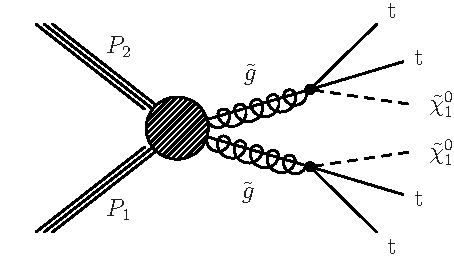
\includegraphics[width=7cm]{figures/Appendices/Ma5ValidationSUS13012/T1tttt.pdf}
\caption{Diagram of the dominant SUSY production mechanism
for the T1tttt signal model.}
\label{fig:T1tttt}
\end{figure}

    \begin{table}[h!]
    \begin{centering}
    \begin{tabular}{  c | c | c  }
    \hline
    \hline
    Cut Name & Official Count (Eff) & MA5 Count (Eff)\\
    \hline
        MET Cleaning & 190.5 (xxx) & 190.5 (xxx)\\
    No Lepton & 95.9 (50\%) & 101.04 (53\%)\\
    NJets$>$2 & 95.8 (99\%) & 100.87 (99\%)\\
    $H_T$$>$500 & 95.1 (99\%) & 100.01 (99\%)\\
    \MHT$>$200 & 75.4 (79\%) & 81.23 (81\%)\\
    Min $\Delta(\phi)$ & 62.3 (82\%) & 66.92 (82\%)\\
\hline
\hline
    \end{tabular}
    \caption{The cut flow for the baseline selection in CMS SUS-13-012 for
    the T1tttt working point $(m_{\tilde g},\,m_{\tilde\chi^0_1})=(1100,\,125)$~GeV.  
    The second column is the official account as reported by
    https://twiki.cern.ch/twiki/pub/CMSPublic/PhysicsResultsSUS13012/T1tttt.pdf,
    and our own results are given in column 3. The official counts are
    normalized to luminosity ${\cal L}=19.5$/fb and cross section $\sigma= 10.17$~pb, and our
    counts are normalized to match the official count after the first cut, MET
    Cleaning.}
    \label{table:CF2}
    \end{centering}
    \end{table}
    
    \begin{table}
    \begin{centering}
    \begin{tabular}{  l | c | c  }
    \hline
    \hline
    Signal Region Name & Official & MA5\\
    \hline
    NJets3-5,  $H_T$500-800,  \MHT200-300 & 0.8 & 0.85\\ 
 \hline 
NJets3-5,  $H_T$500-800,  \MHT300-450 & 1.4 & 1.22\\ 
 \hline 
NJets3-5,  $H_T$500-800,  \MHT450-600 & 0.8 & 0.85\\ 
 \hline 
NJets3-5,  $H_T$500-800,  \MHT$>$600 & 0.2 & 0.31\\ 
 \hline 
NJets3-5,  $H_T$800-1000,  \MHT200-300 & 0.5 & 0.45\\ 
 \hline 
NJets3-5,  $H_T$800-1000,  \MHT300-450 & 0.7 & 1.00\\ 
 \hline 
NJets3-5,  $H_T$800-1000,  \MHT450-600 & 1.0 & 1.03\\ 
 \hline 
NJets3-5,  $H_T$800-1000,  \MHT$>$600 & 0.8 & 0.79\\ 
 \hline 
NJets3-5,  $H_T$1000-1250,  \MHT200-300 & 0.5 & 0.53\\ 
 \hline 
NJets3-5,  $H_T$1000-1250,  \MHT300-450 & 1.0 & 0.83\\ 
 \hline 
NJets3-5,  $H_T$1000-1250,  \MHT450-600 & 0.8 & 0.87\\ 
 \hline 
NJets3-5,  $H_T$1000-1250,  \MHT$>$600 & 0.9 & 1.01\\ 
 \hline 
NJets3-5,  $H_T$1250-1500,  \MHT200-300 & 0.4 & 0.40\\ 
 \hline 
NJets3-5,  $H_T$1250-1500,  \MHT300-450 & 0.5 & 0.58\\ 
 \hline 
NJets3-5,  $H_T$1250-1500,  \MHT$>$450 & 0.8 & 0.81\\ 
 \hline 
NJets3-5,  $H_T$$>$1500,  \MHT200-300 & 0.3 & 0.34\\ 
 \hline 
NJets3-5,  $H_T$$>$1500,  \MHT$>$300 & 0.9 & 1.01\\ 
 \hline 
NJets6-7,  $H_T$500-800,  \MHT200-300 & 0.9 & 0.81\\ 
 \hline 
NJets6-7,  $H_T$500-800,  \MHT300-450 & 1.2 & 0.85\\ 
 \hline 
NJets6-7,  $H_T$500-800,  \MHT$>$450 & 0.6 & 0.44\\ 
 \hline 
NJets6-7,  $H_T$800-1000,  \MHT200-300 & 1.5 & 1.16\\ 
 \hline 
NJets6-7,  $H_T$800-1000,  \MHT300-450 & 2.5 & 2.35\\ 
 \hline 
NJets6-7,  $H_T$800-1000,  \MHT$>$450 & 2.5 & 2.59\\ 
 \hline 
NJets6-7,  $H_T$1000-1250,  \MHT200-300 & 1.8 & 1.71\\ 
 \hline 
NJets6-7,  $H_T$1000-1250,  \MHT300-450 & 3.4 & 3.37\\ 
 \hline 
NJets6-7,  $H_T$1000-1250,  \MHT$>$450 & 4.5 & 5.21\\ 
 \hline 
NJets6-7,  $H_T$1250-1500,  \MHT200-300 & 1.4 & 1.46\\ 
 \hline 
NJets6-7,  $H_T$1250-1500,  \MHT300-450 & 2.2 & 2.43\\ 
 \hline 
NJets6-7,  $H_T$1250-1500,  \MHT$>$450 & 2.8 & 3.34\\ 
 \hline 
NJets6-7,  $H_T$$>$1500,  \MHT200-300 & 1.1 & 1.16\\ 
 \hline 
NJets6-7,  $H_T$$>$1500,  \MHT$>$300 & 3.4 & 3.99\\ 
 \hline 
NJets$>$7,  $H_T$500-800,  \MHT$>$200 & 0.2 & 0.15\\ 
 \hline 
NJets$>$7,  $H_T$800-1000,  \MHT$>$200 & 1.9 & 1.69\\ 
 \hline 
NJets$>$7,  $H_T$1000-1250,  \MHT$>$200 & 5.7 & 6.37\\ 
 \hline 
NJets$>$7,  $H_T$1250-1500,  \MHT$>$200 & 5.9 & 7.28\\ 
 \hline 
NJets$>$7,  $H_T$$>$1500,  \MHT$>$200 & 6.0 & 7.53\\ 
 \hline 
\hline
    \end{tabular}
    \caption{The signal region (SR) counts in CMS SUS-13-012 for the T1tttt scenario 
    after all selection has been applied. Column 2 is the official account obtained through generous correspondence with Christian Sanders,
    and our own results displayed in column 3. These counts were determined by applying the SR selection to the end of the cut flow featured in table \ref{table:CF2}.}
    \end{centering}
    \end{table}
    
\begin{figure}
        \centering
        \subfloat[]{
                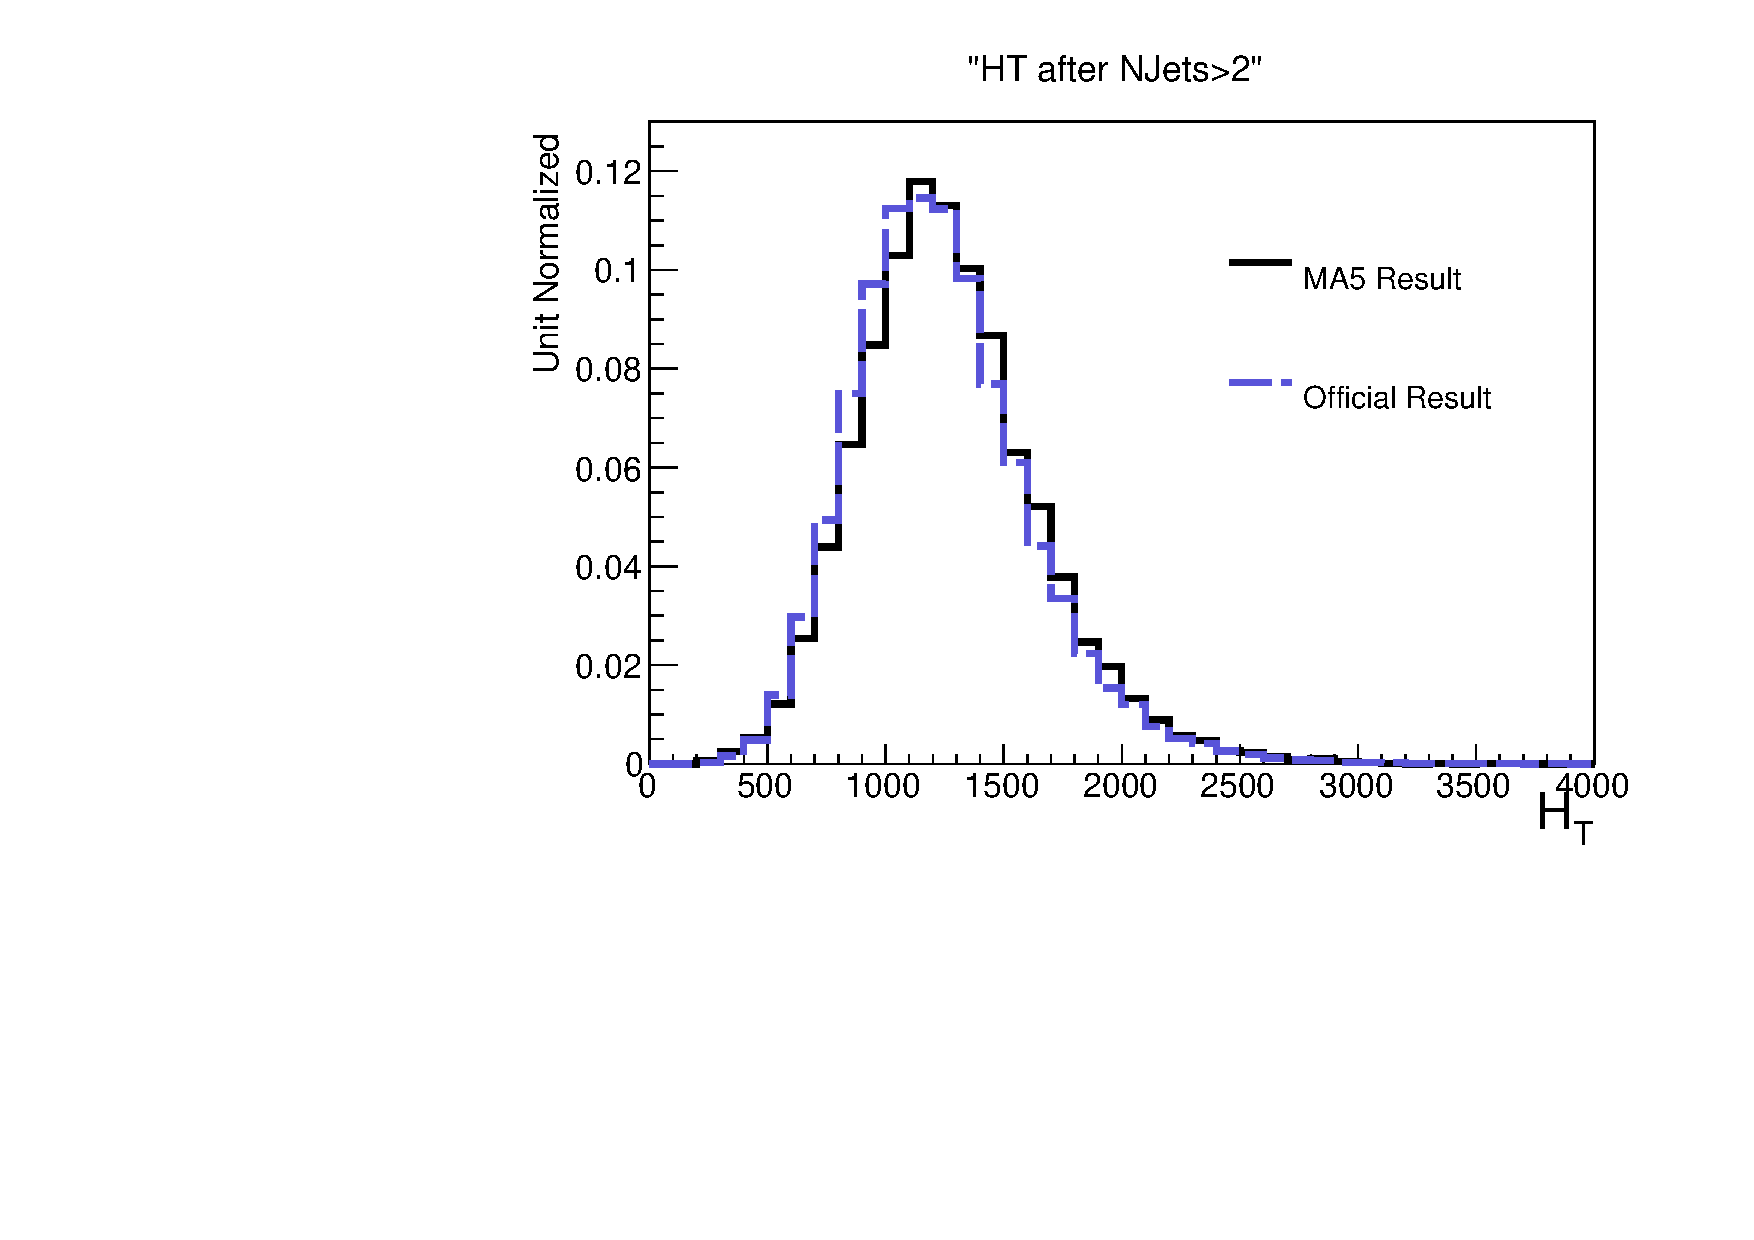
\includegraphics[width=0.5\textwidth]{figures/Appendices/Ma5ValidationSUS13012/T1tttt_HT_after_NJets>2.pdf}
                \label{fig:gull}
        }%
        \hspace{-1 cm}
        ~ %add desired spacing between images, e. g. ~, \quad, \qquad, \hfill etc.
          %(or a blank line to force the subfigure onto a new line)
        \subfloat[]{
                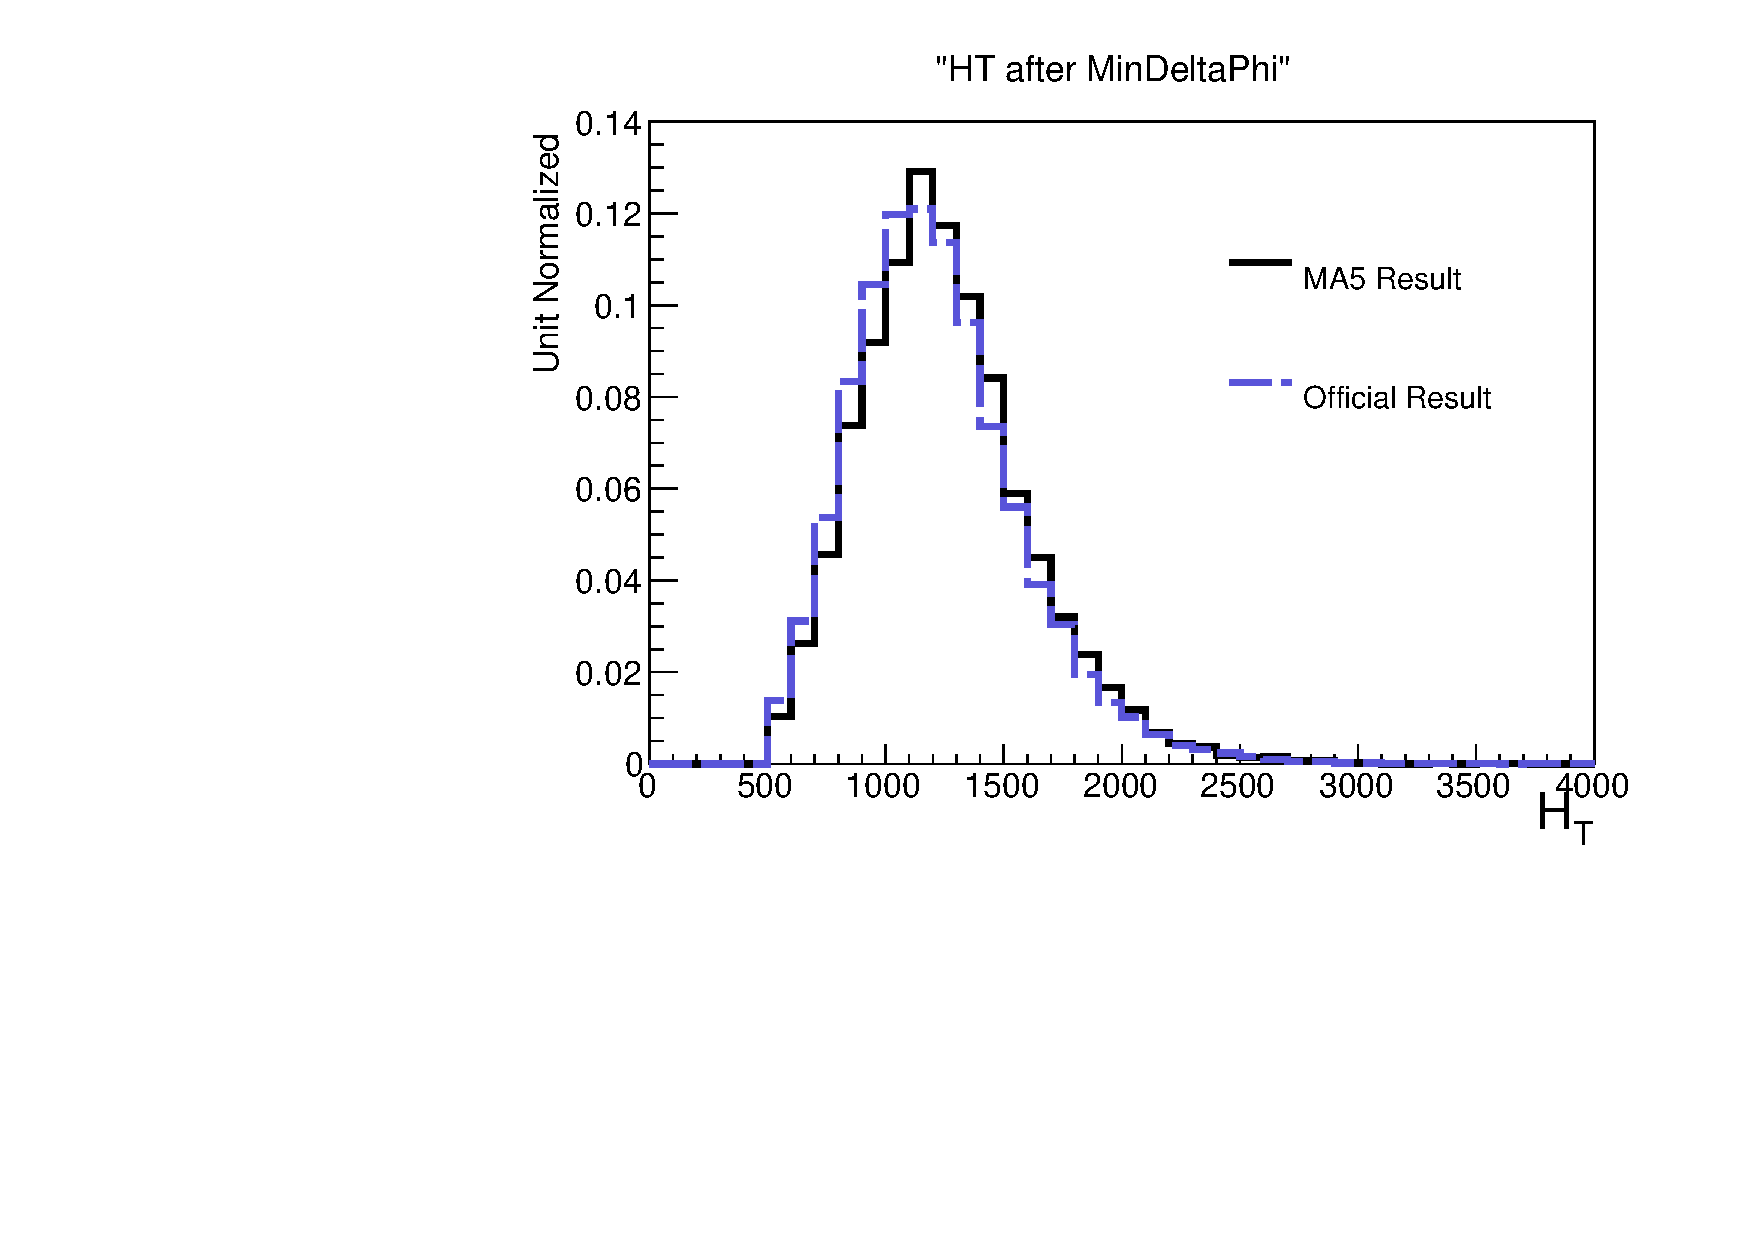
\includegraphics[width=0.5\textwidth]{figures/Appendices/Ma5ValidationSUS13012/T1tttt_HT_after_MinDeltaPhi.pdf}
                \label{fig:tiger}
        }
        \caption{Comparison of the distributions of $H_T$ between the official and our own samples after the ``n-1" cut, Min $\Delta(\phi)$ (left), and after all baseline cuts (right), for the T1tttt signal model.}\label{fig:animals}
\end{figure}        
        
\begin{figure}
        \centering
        \subfloat[]{
                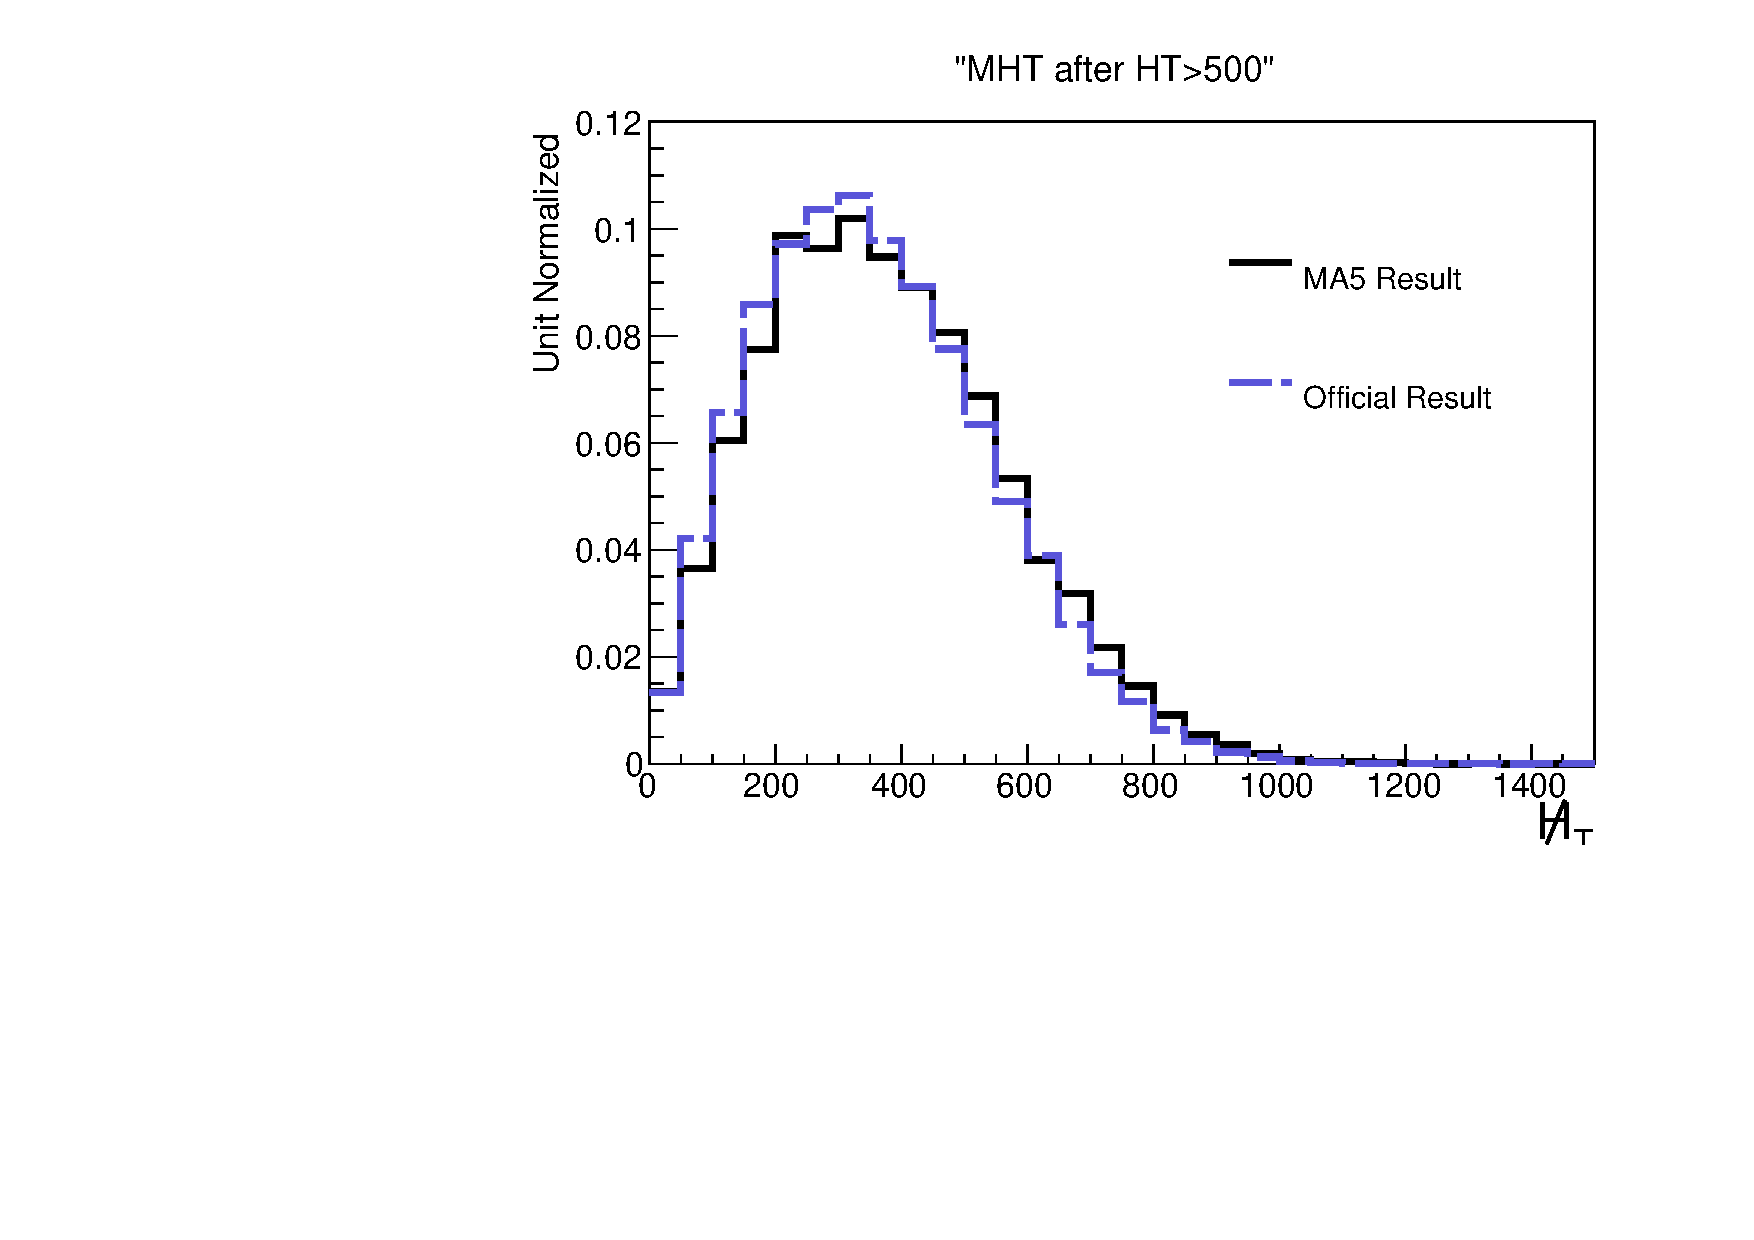
\includegraphics[width=0.5\textwidth]{figures/Appendices/Ma5ValidationSUS13012/T1tttt_MHT_after_HT>500.pdf}
                \label{fig:gull}
        }%
        \hspace{-1 cm}
        ~ %add desired spacing between images, e. g. ~, \quad, \qquad, \hfill etc.
          %(or a blank line to force the subfigure onto a new line)
        \subfloat[]{
                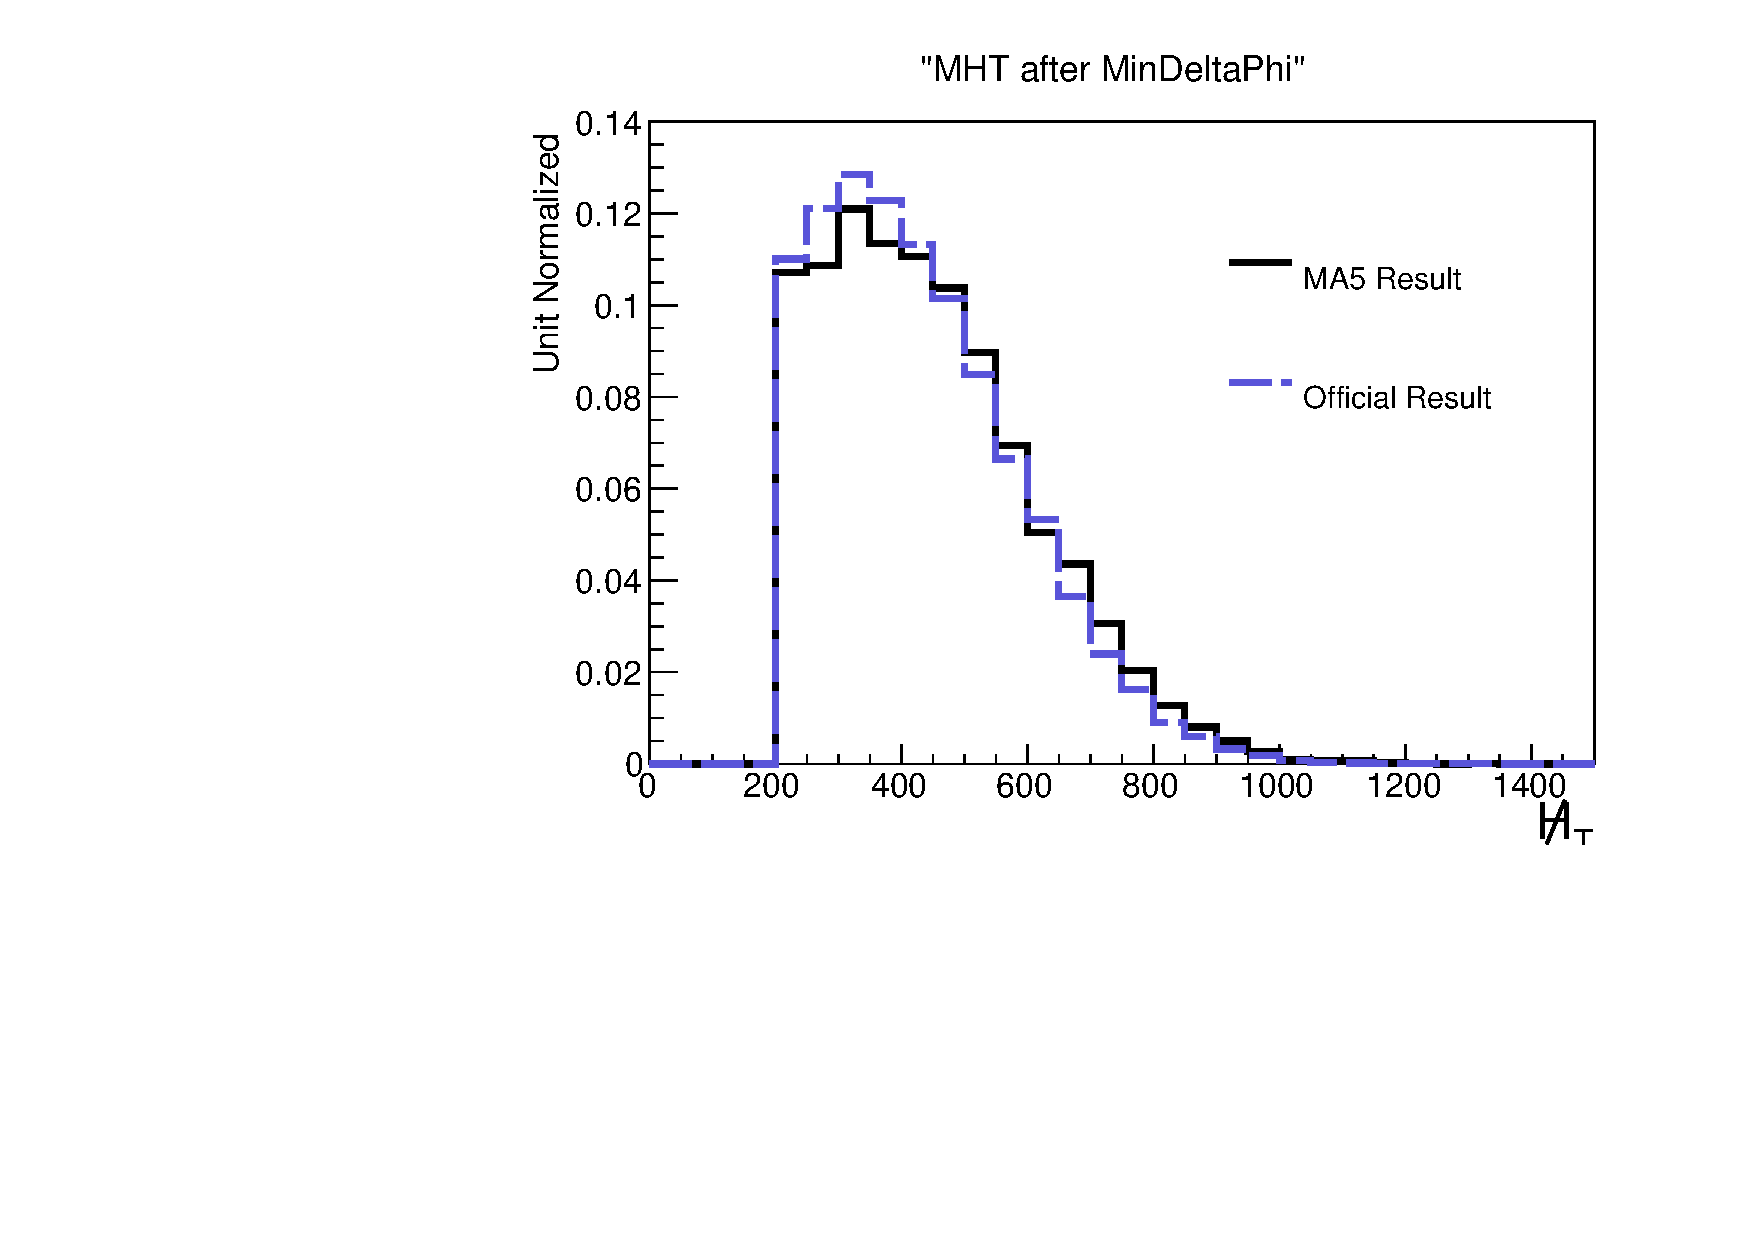
\includegraphics[width=0.5\textwidth]{figures/Appendices/Ma5ValidationSUS13012/T1tttt_MHT_after_MinDeltaPhi.pdf}
                \label{fig:tiger}
        }
        \caption{Comparison of the distributions of \MHT between the official and our own samples after the ``n-1" cut, Min $\Delta(\phi)$ (left), and after all baseline cuts (right), for the T1tttt signal model.}\label{fig:animals}
\end{figure}        
        
\begin{figure}
        \centering
        \subfloat[]{
                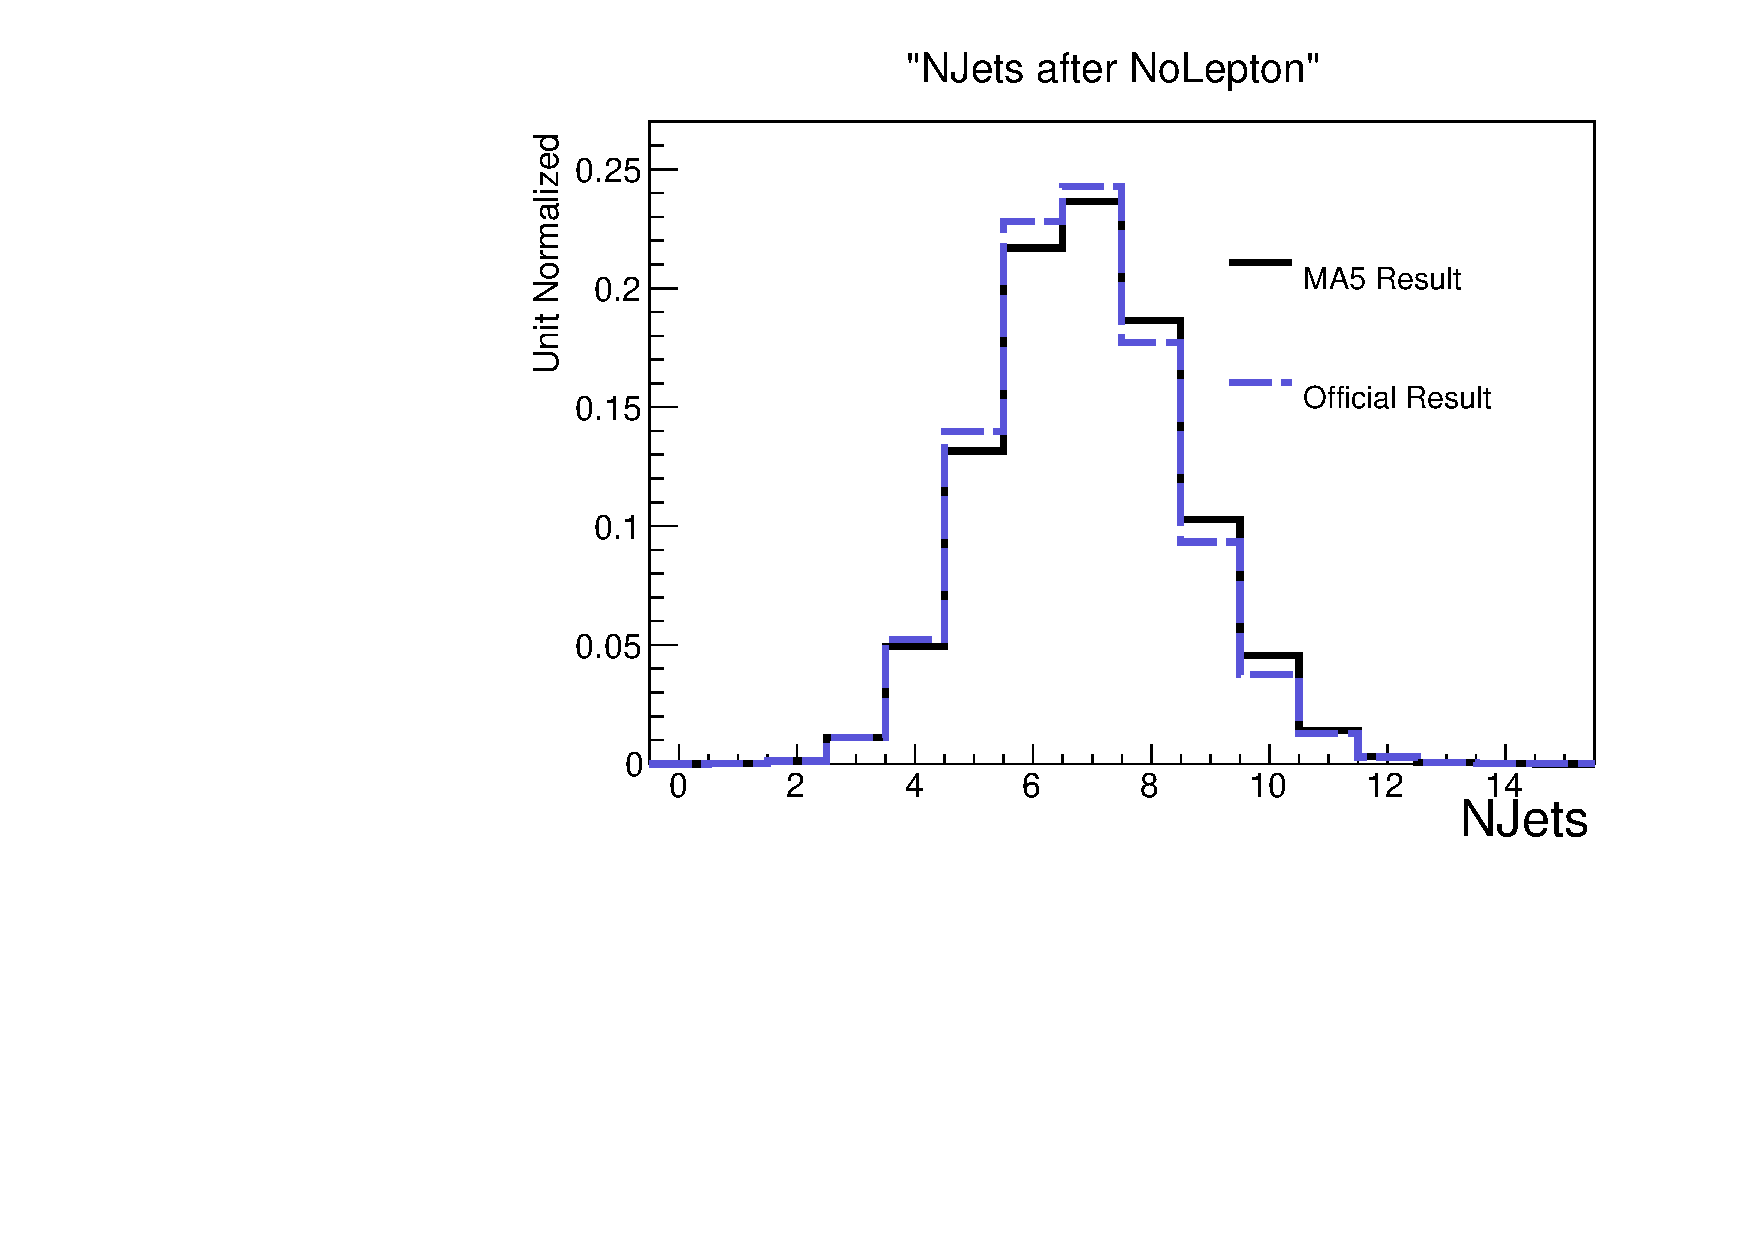
\includegraphics[width=0.5\textwidth]{figures/Appendices/Ma5ValidationSUS13012/T1tttt_NJets_after_NoLepton.pdf}
                \label{fig:gull}
        }%
        \hspace{-1 cm}
        ~ %add desired spacing between images, e. g. ~, \quad, \qquad, \hfill etc.
          %(or a blank line to force the subfigure onto a new line)
        \subfloat[]{
                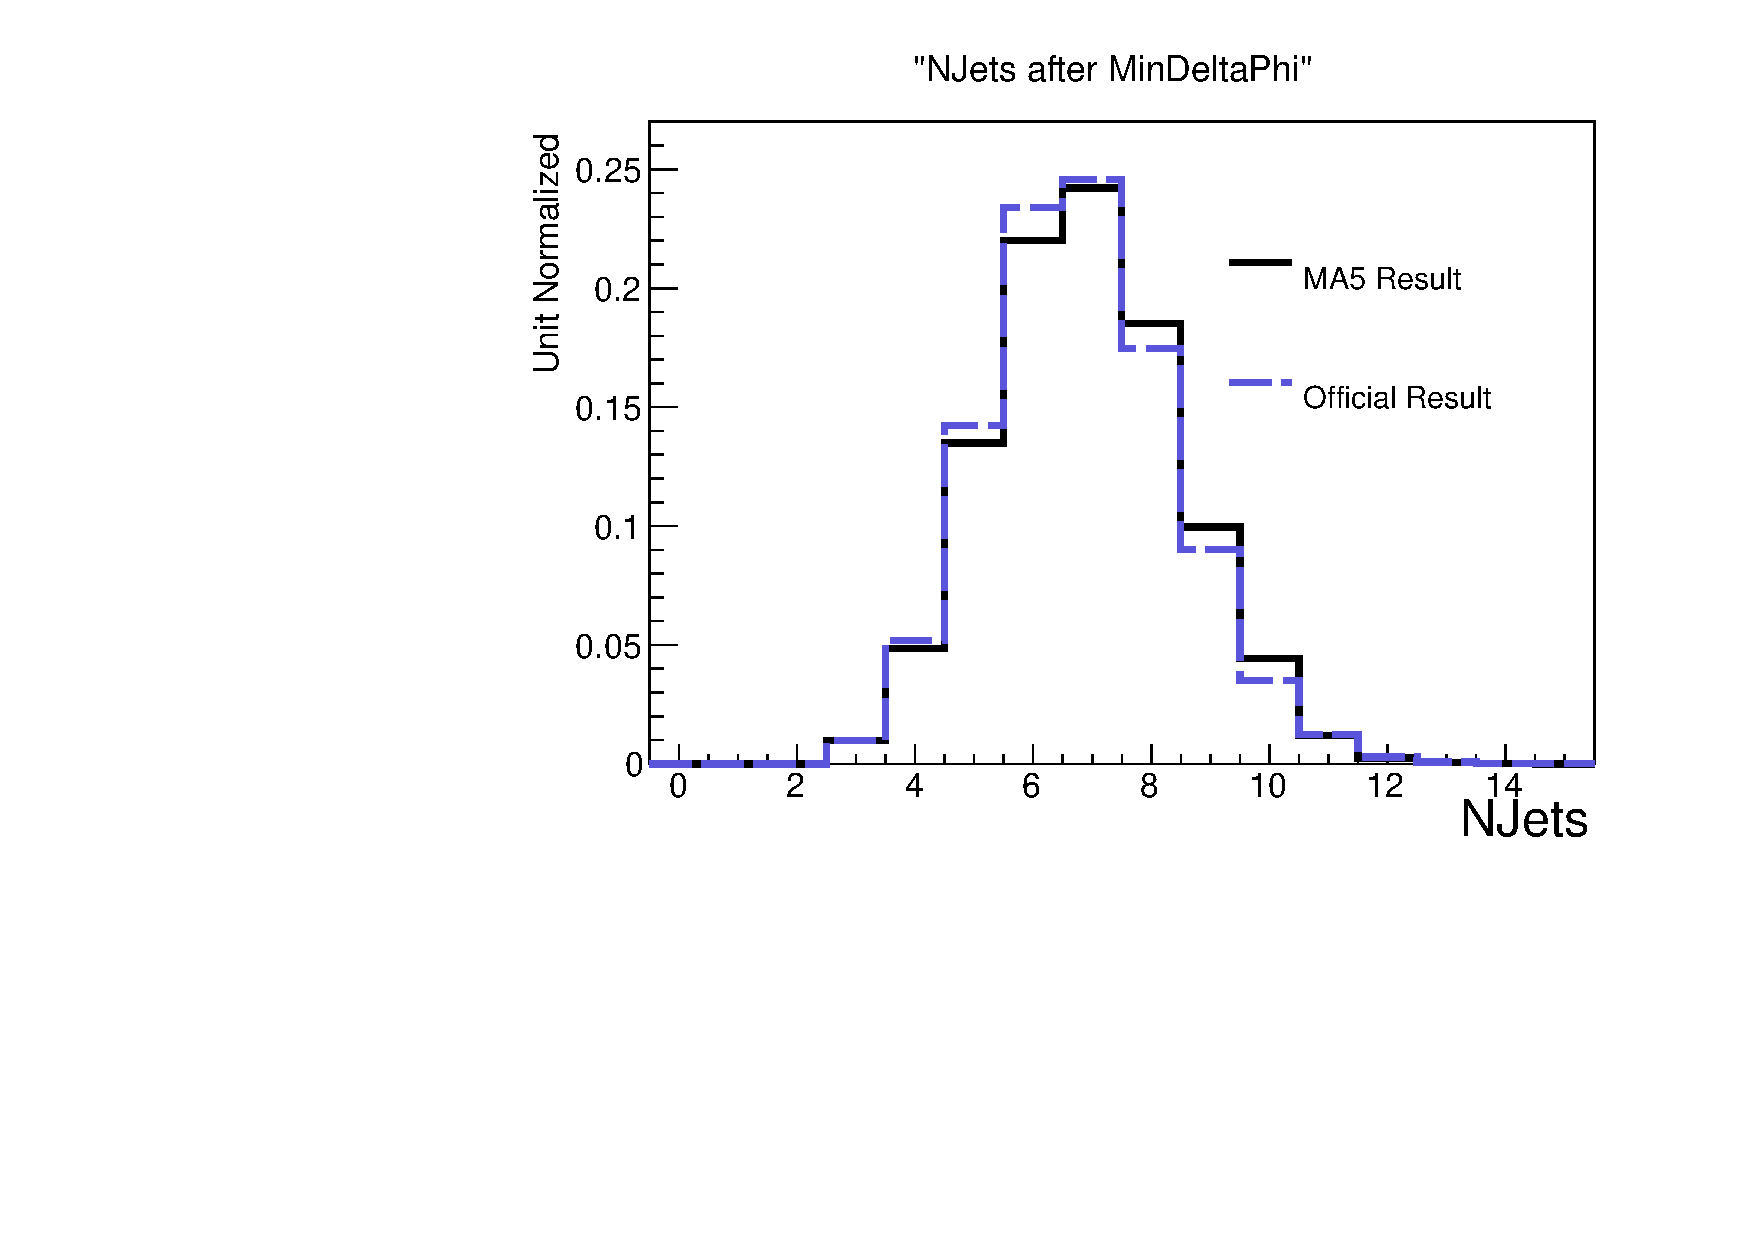
\includegraphics[width=0.5\textwidth]{figures/Appendices/Ma5ValidationSUS13012/T1tttt_NJets_after_MinDeltaPhi.pdf}
                \label{fig:tiger}
        }
        \caption{Comparison of the distributions of NJets between the official and our own samples after the ``n-1" cut, Min $\Delta(\phi)$ (left), and after all baseline cuts (right), for the T1tttt signal model.}\label{fig:animals}
\end{figure}        
        
        \begin{figure}
        \centering
        \subfloat[]{
        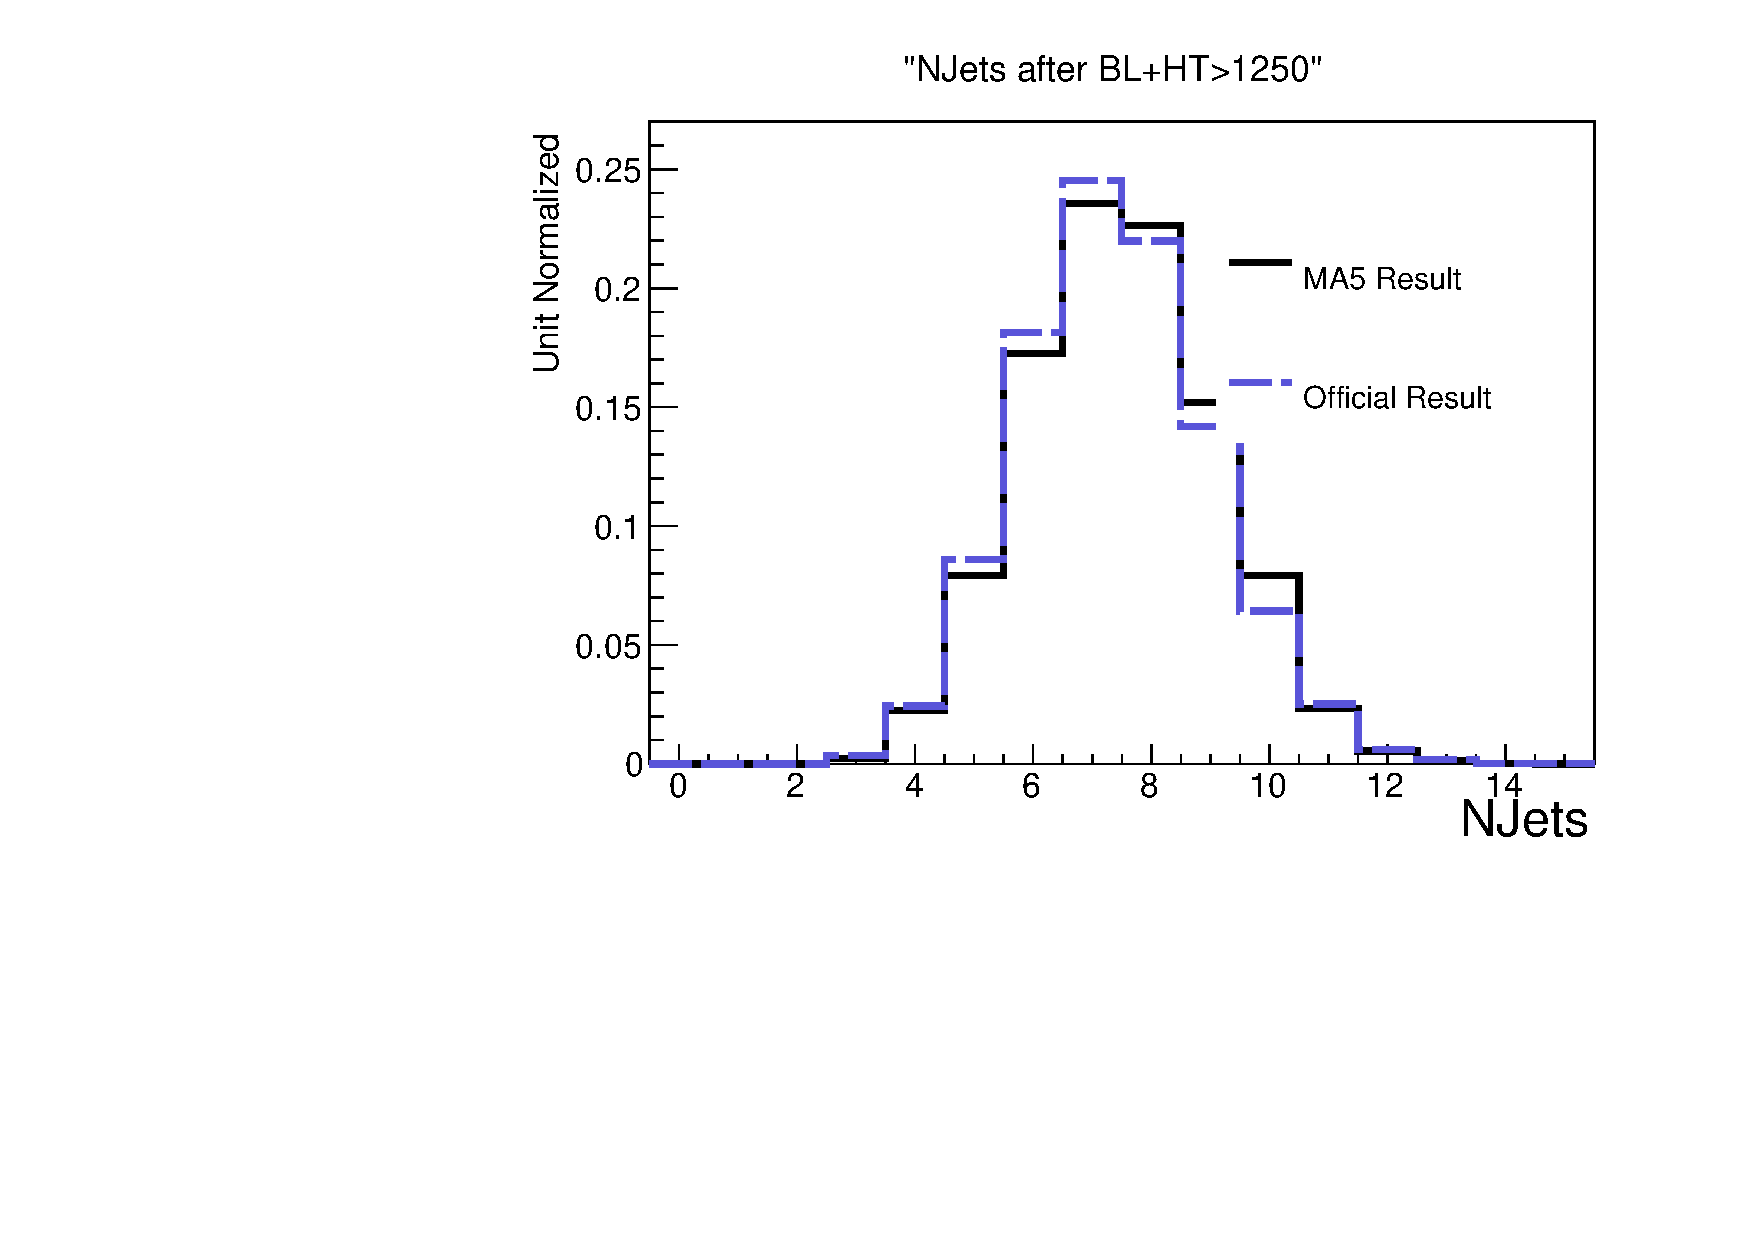
\includegraphics[width=0.5\textwidth]{figures/Appendices/Ma5ValidationSUS13012/T1tttt_NJets_after_BL+HT>1250.pdf}
        \label{fig:gull}
        }%
        \hspace{-1 cm}
        ~ %add desired spacing between images, e. g. ~, \quad, \qquad, \hfill etc.
        %(or a blank line to force the subfigure onto a new line)
        \subfloat[]{
        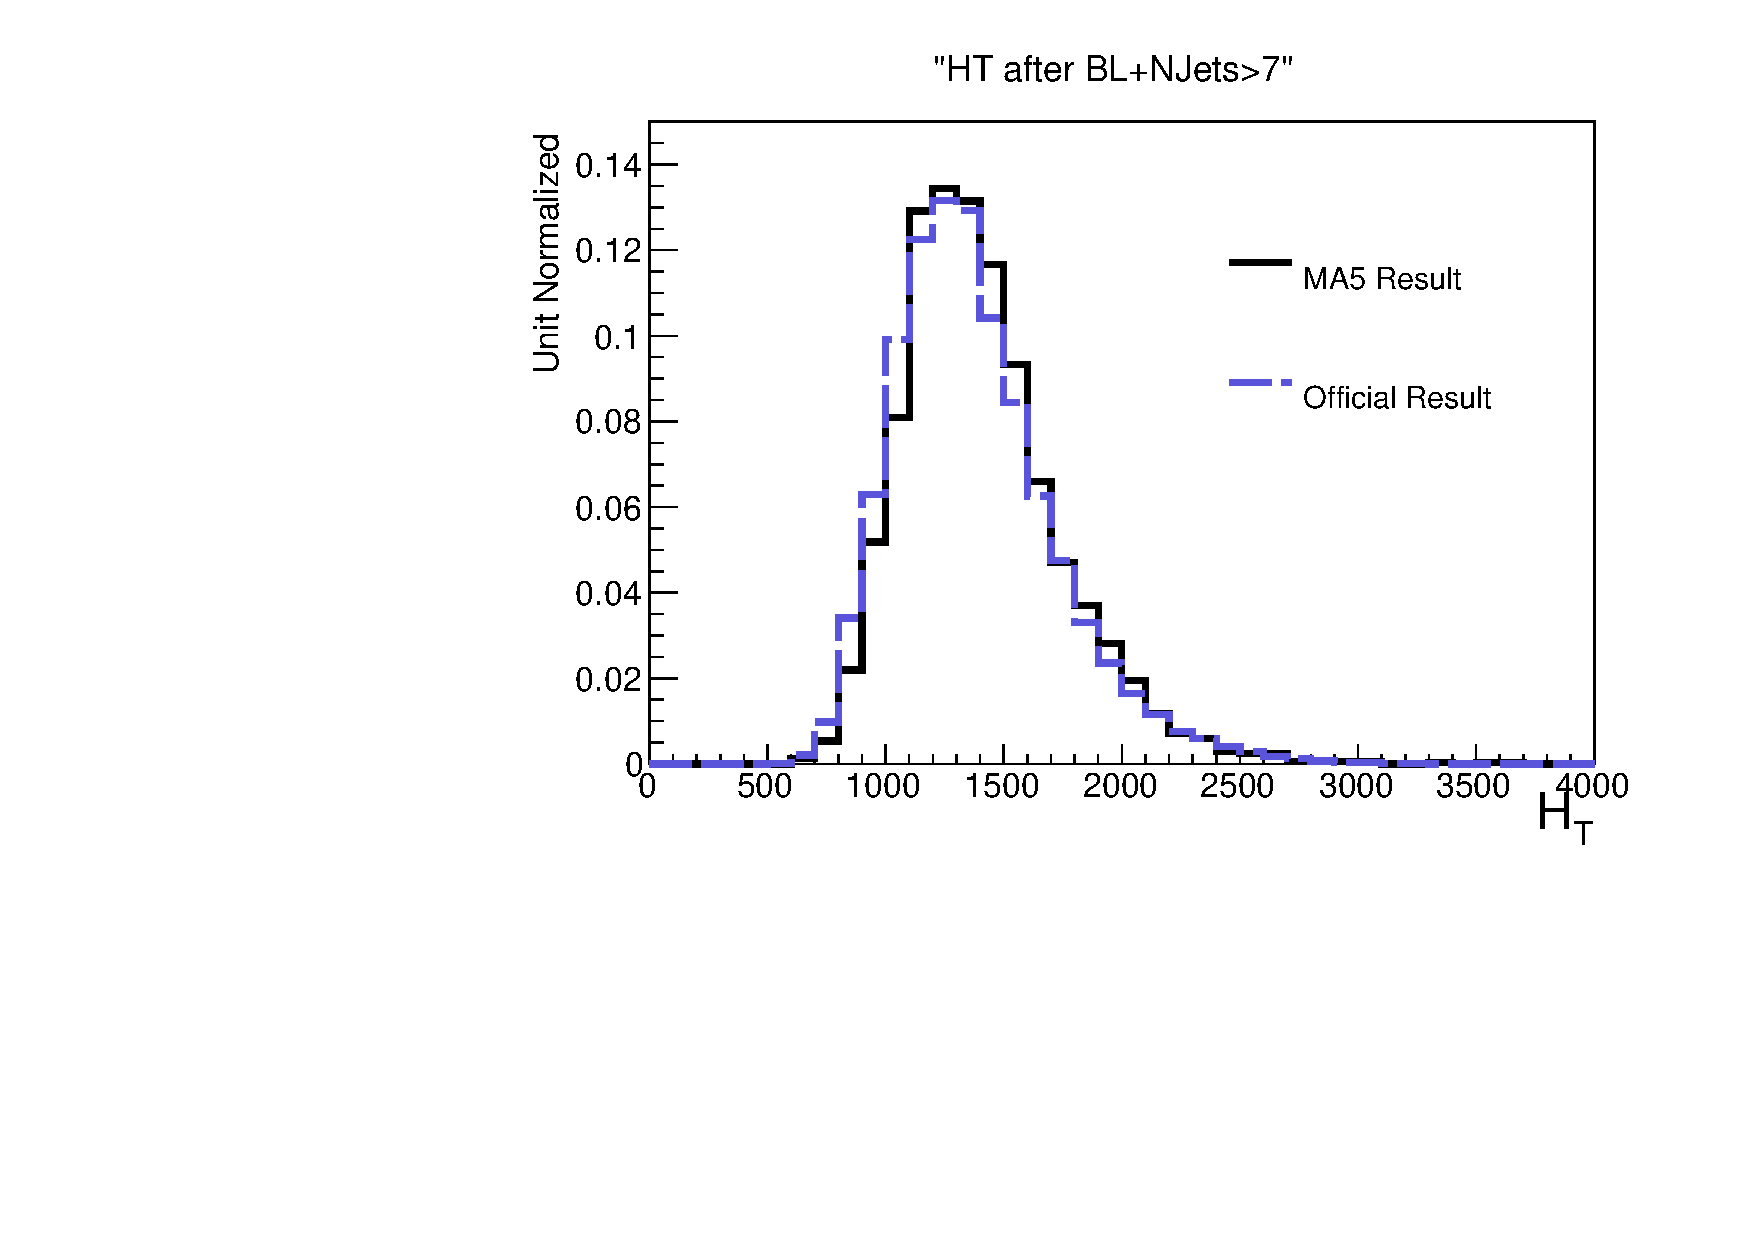
\includegraphics[width=0.5\textwidth]{figures/Appendices/Ma5ValidationSUS13012/T1tttt_HT_after_BL+NJets>7.pdf}
        \label{fig:tiger}
        }
        \caption{Additional checks: comparison between ours and the official distributions of NJets after BL+$H_T$$>$1250 cuts (left), and $H_T$ after BL+NJets$>$7 cuts (right), for the T1tttt signal model.}
        \end{figure}  
        

\clearpage
%%%%%%%%%%%%%%%%%%%%%%%%%%%%%%%%%%%%%%%%%%%%%%%%%
\subsection{T5VV simplified model}
%%%%%%%%%%%%%%%%%%%%%%%%%%%%%%%%%%%%%%%%%%%%%%%%%

\begin{figure}[h!]
\centering
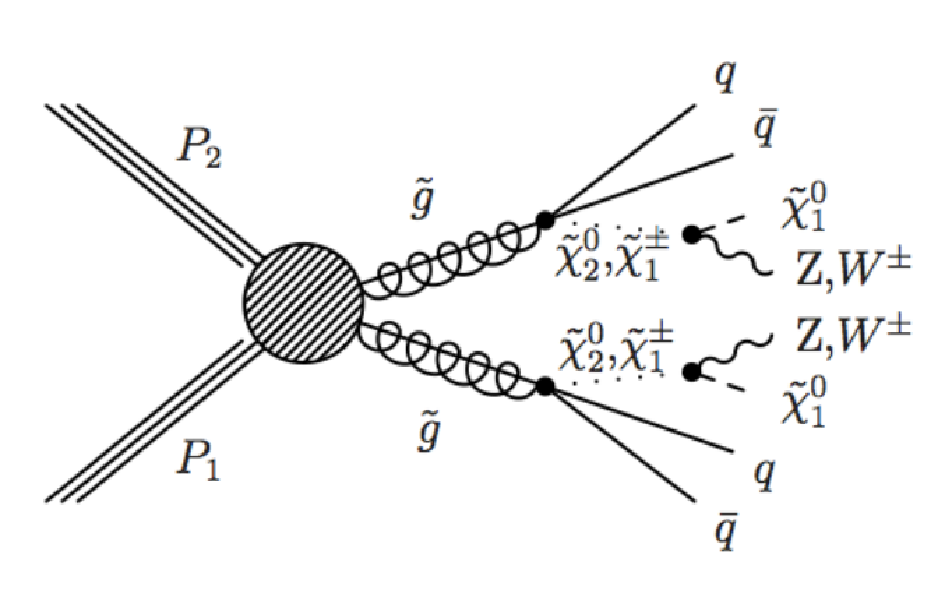
\includegraphics[width=7cm]{figures/Appendices/Ma5ValidationSUS13012/T5VV.pdf}
\caption{Diagram of the dominant SUSY production mechanism
for the T5VV signal model.}
\label{fig:T5VV}
\end{figure}

    \begin{table}[h!]
    \begin{centering}
    \begin{tabular}{  c | c | c  }
    \hline
    \hline
    Cut Name & Official Count (Eff) & MA5 Count (Eff)\\
    \hline
        MET Cleaning & 189.9 (xxx) & 189.9 (xxx)\\
    No Lepton & 136.2 (71\%) & 142.07 (74\%)\\
    NJets$>$2 & 135.9 (99\%) & 141.69 (99\%)\\
    $H_T$$>$500 & 135.5 (99\%) & 141.26 (99\%)\\
    \MHT$>$200 & 108.8 (80\%) & 115.23 (81\%)\\
    Min $\Delta(\phi)$ & 89.6 (82\%) & 95.22 (82\%)\\
\hline
\hline
    \end{tabular}
    \caption{The cut flow for the baseline selection in CMS SUS-13-012 for
    the T5VV working point $(m_{\tilde g},\,m_{\tilde\chi^0_1})=(1100,\,125)$~GeV.  
    The second column is the official account as reported by
    https://twiki.cern.ch/twiki/pub/CMSPublic/PhysicsResultsSUS13012/T5VV.pdf,
    and our own results are given in column 3. The official counts are
    normalized to luminosity ${\cal L}=19.5$/fb and cross section $\sigma= 10.17$~pb, and our
    counts are normalized to match the official count after the first cut, MET
    Cleaning.}
    \label{table:CF3}
    \end{centering}
    \end{table}
    
    \begin{table}
    \begin{centering}
    \begin{tabular}{  l | c | c  }
    \hline
    \hline
    Signal Region Name & Official & MA5\\
    \hline
    NJets3-5,  $H_T$500-800,  \MHT200-300 & 1.0 & 1.18\\ 
 \hline 
NJets3-5,  $H_T$500-800,  \MHT300-450 & 1.8 & 1.77\\ 
 \hline 
NJets3-5,  $H_T$500-800,  \MHT450-600 & 1.1 & 1.09\\ 
 \hline 
NJets3-5,  $H_T$500-800,  \MHT$>$600 & 0.3 & 0.31\\ 
 \hline 
NJets3-5,  $H_T$800-1000,  \MHT200-300 & 1.5 & 1.08\\ 
 \hline 
NJets3-5,  $H_T$800-1000,  \MHT300-450 & 1.7 & 2.40\\ 
 \hline 
NJets3-5,  $H_T$800-1000,  \MHT450-600 & 2.1 & 2.12\\ 
 \hline 
NJets3-5,  $H_T$800-1000,  \MHT$>$600 & 1.2 & 1.43\\ 
 \hline 
NJets3-5,  $H_T$1000-1250,  \MHT200-300 & 1.9 & 1.84\\ 
 \hline 
NJets3-5,  $H_T$1000-1250,  \MHT300-450 & 3.1 & 3.23\\ 
 \hline 
NJets3-5,  $H_T$1000-1250,  \MHT450-600 & 2.8 & 2.66\\ 
 \hline 
NJets3-5,  $H_T$1000-1250,  \MHT$>$600 & 2.1 & 2.41\\ 
 \hline 
NJets3-5,  $H_T$1250-1500,  \MHT200-300 & 1.3 & 1.35\\ 
 \hline 
NJets3-5,  $H_T$1250-1500,  \MHT300-450 & 2.3 & 2.03\\ 
 \hline 
NJets3-5,  $H_T$1250-1500,  \MHT$>$450 & 3.2 & 3.67\\ 
 \hline 
NJets3-5,  $H_T$$>$1500,  \MHT200-300 & 1.1 & 1.06\\ 
 \hline 
NJets3-5,  $H_T$$>$1500,  \MHT$>$300 & 3.7 & 3.77\\ 
 \hline 
NJets6-7,  $H_T$500-800,  \MHT200-300 & 0.4 & 0.29\\ 
 \hline 
NJets6-7,  $H_T$500-800,  \MHT300-450 & 0.4 & 0.32\\ 
 \hline 
NJets6-7,  $H_T$500-800,  \MHT$>$450 & 0.2 & 0.15\\ 
 \hline 
NJets6-7,  $H_T$800-1000,  \MHT200-300 & 1.2 & 1.06\\ 
 \hline 
NJets6-7,  $H_T$800-1000,  \MHT300-450 & 1.9 & 1.73\\ 
 \hline 
NJets6-7,  $H_T$800-1000,  \MHT$>$450 & 1.7 & 1.65\\ 
 \hline 
NJets6-7,  $H_T$1000-1250,  \MHT200-300 & 3.1 & 2.66\\ 
 \hline 
NJets6-7,  $H_T$1000-1250,  \MHT300-450 & 4.6 & 4.72\\ 
 \hline 
NJets6-7,  $H_T$1000-1250,  \MHT$>$450 & 5.9 & 5.77\\ 
 \hline 
NJets6-7,  $H_T$1250-1500,  \MHT200-300 & 2.7 & 2.89\\ 
 \hline 
NJets6-7,  $H_T$1250-1500,  \MHT300-450 & 4.4 & 4.72\\ 
 \hline 
NJets6-7,  $H_T$1250-1500,  \MHT$>$450 & 5.8 & 6.57\\ 
 \hline 
NJets6-7,  $H_T$$>$1500,  \MHT200-300 & 2.7 & 3.01\\ 
 \hline 
NJets6-7,  $H_T$$>$1500,  \MHT$>$300 & 9.2 & 10.94\\ 
 \hline 
NJets$>$7,  $H_T$500-800,  \MHT$>$200 & 0.0 & 0.01\\ 
 \hline 
NJets$>$7,  $H_T$800-1000,  \MHT$>$200 & 0.4 & 0.33\\ 
 \hline 
NJets$>$7,  $H_T$1000-1250,  \MHT$>$200 & 2.3 & 2.50\\ 
 \hline 
NJets$>$7,  $H_T$1250-1500,  \MHT$>$200 & 3.8 & 4.48\\ 
 \hline 
NJets$>$7,  $H_T$$>$1500,  \MHT$>$200 & 6.0 & 7.84\\ 
 \hline 
\hline
    \end{tabular}
    \caption{The signal region (SR) counts in CMS SUS-13-012 for the T5VV scenario 
     after all selection has been applied. Column 2 is the official account obtained through generous correspondence with Christian Sanders,
    and our own results displayed in column 3. These counts were determined by applying the SR selection to the end of the cut flow featured in table \ref{table:CF3}.}
    \end{centering}
    \end{table}
    
\begin{figure}
        \centering
        \subfloat[]{
                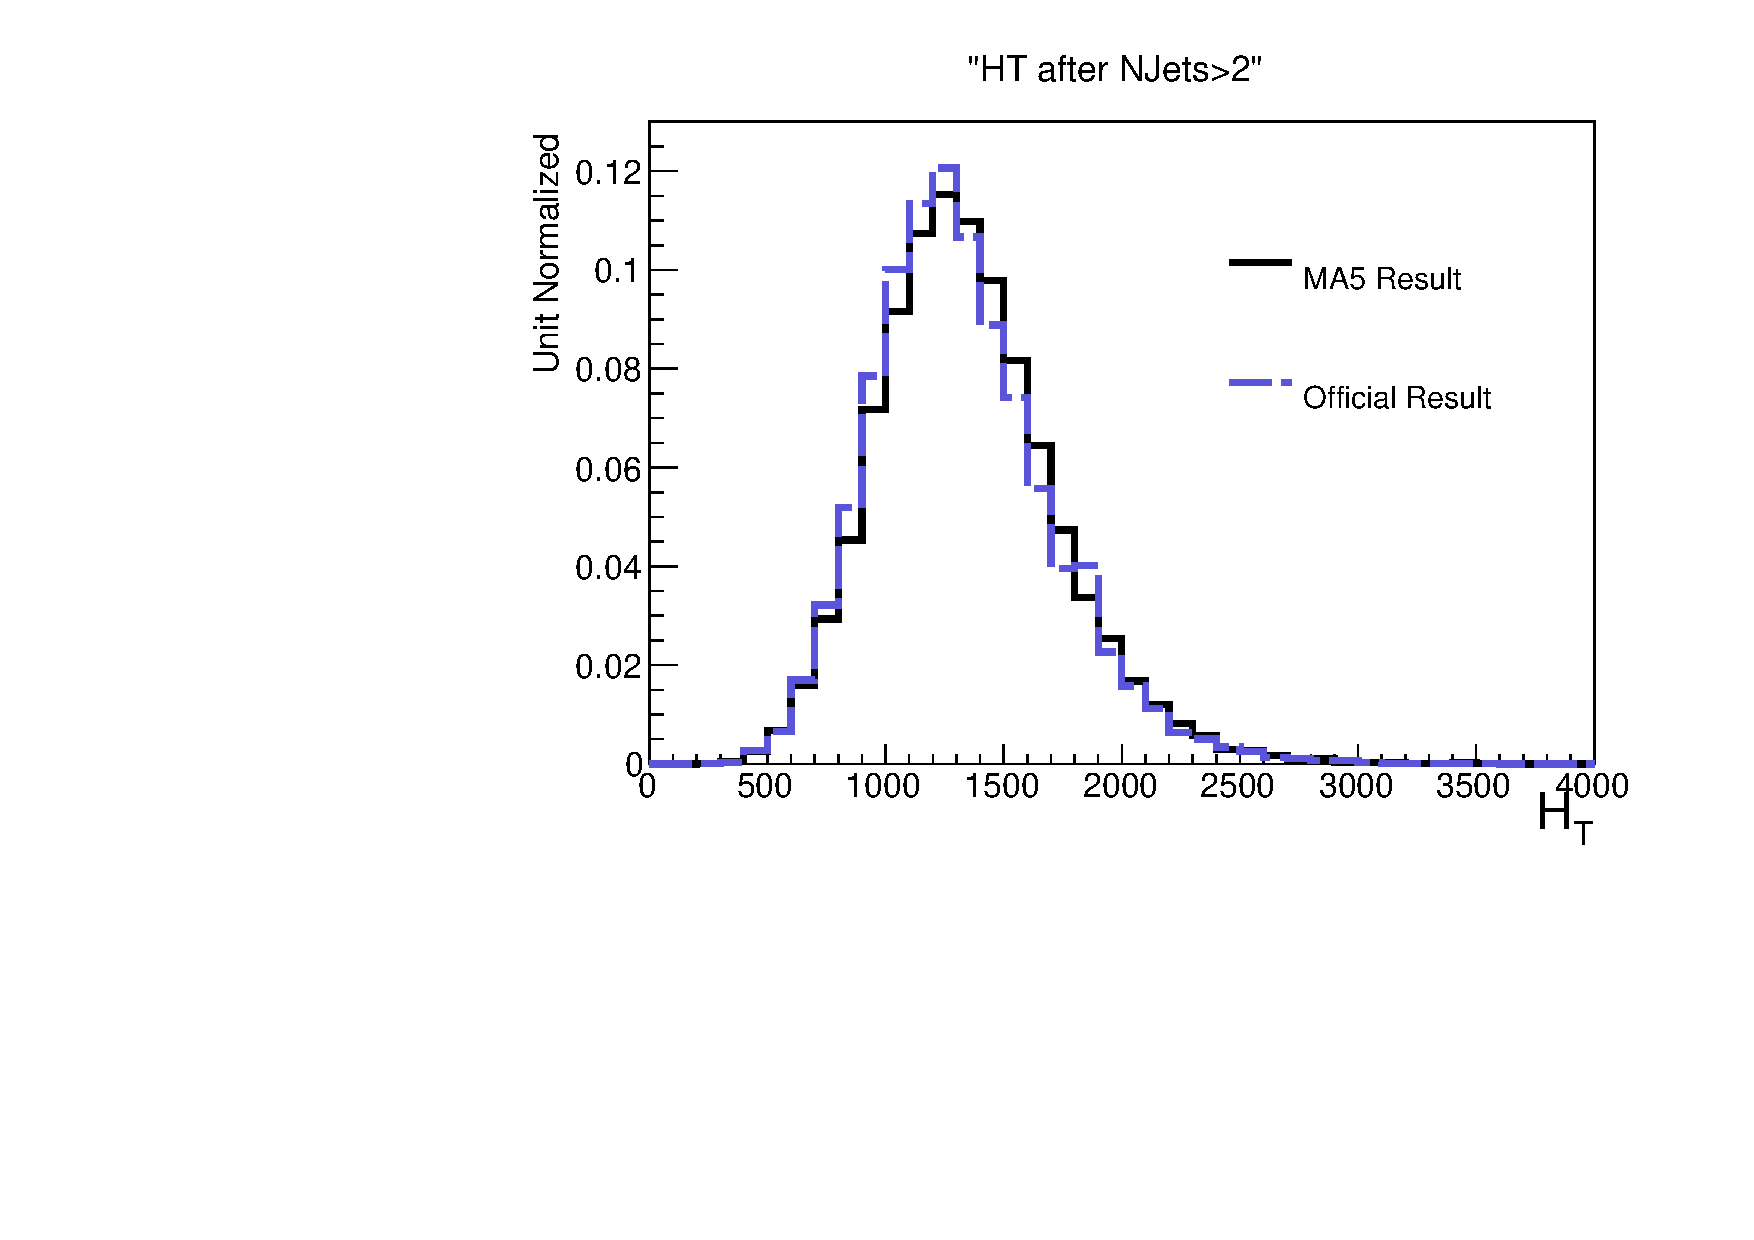
\includegraphics[width=0.5\textwidth]{figures/Appendices/Ma5ValidationSUS13012/T5VV_HT_after_NJets>2.pdf}
                \label{fig:gull}
        }%
        \hspace{-1 cm}
        ~ %add desired spacing between images, e. g. ~, \quad, \qquad, \hfill etc.
          %(or a blank line to force the subfigure onto a new line)
        \subfloat[]{
                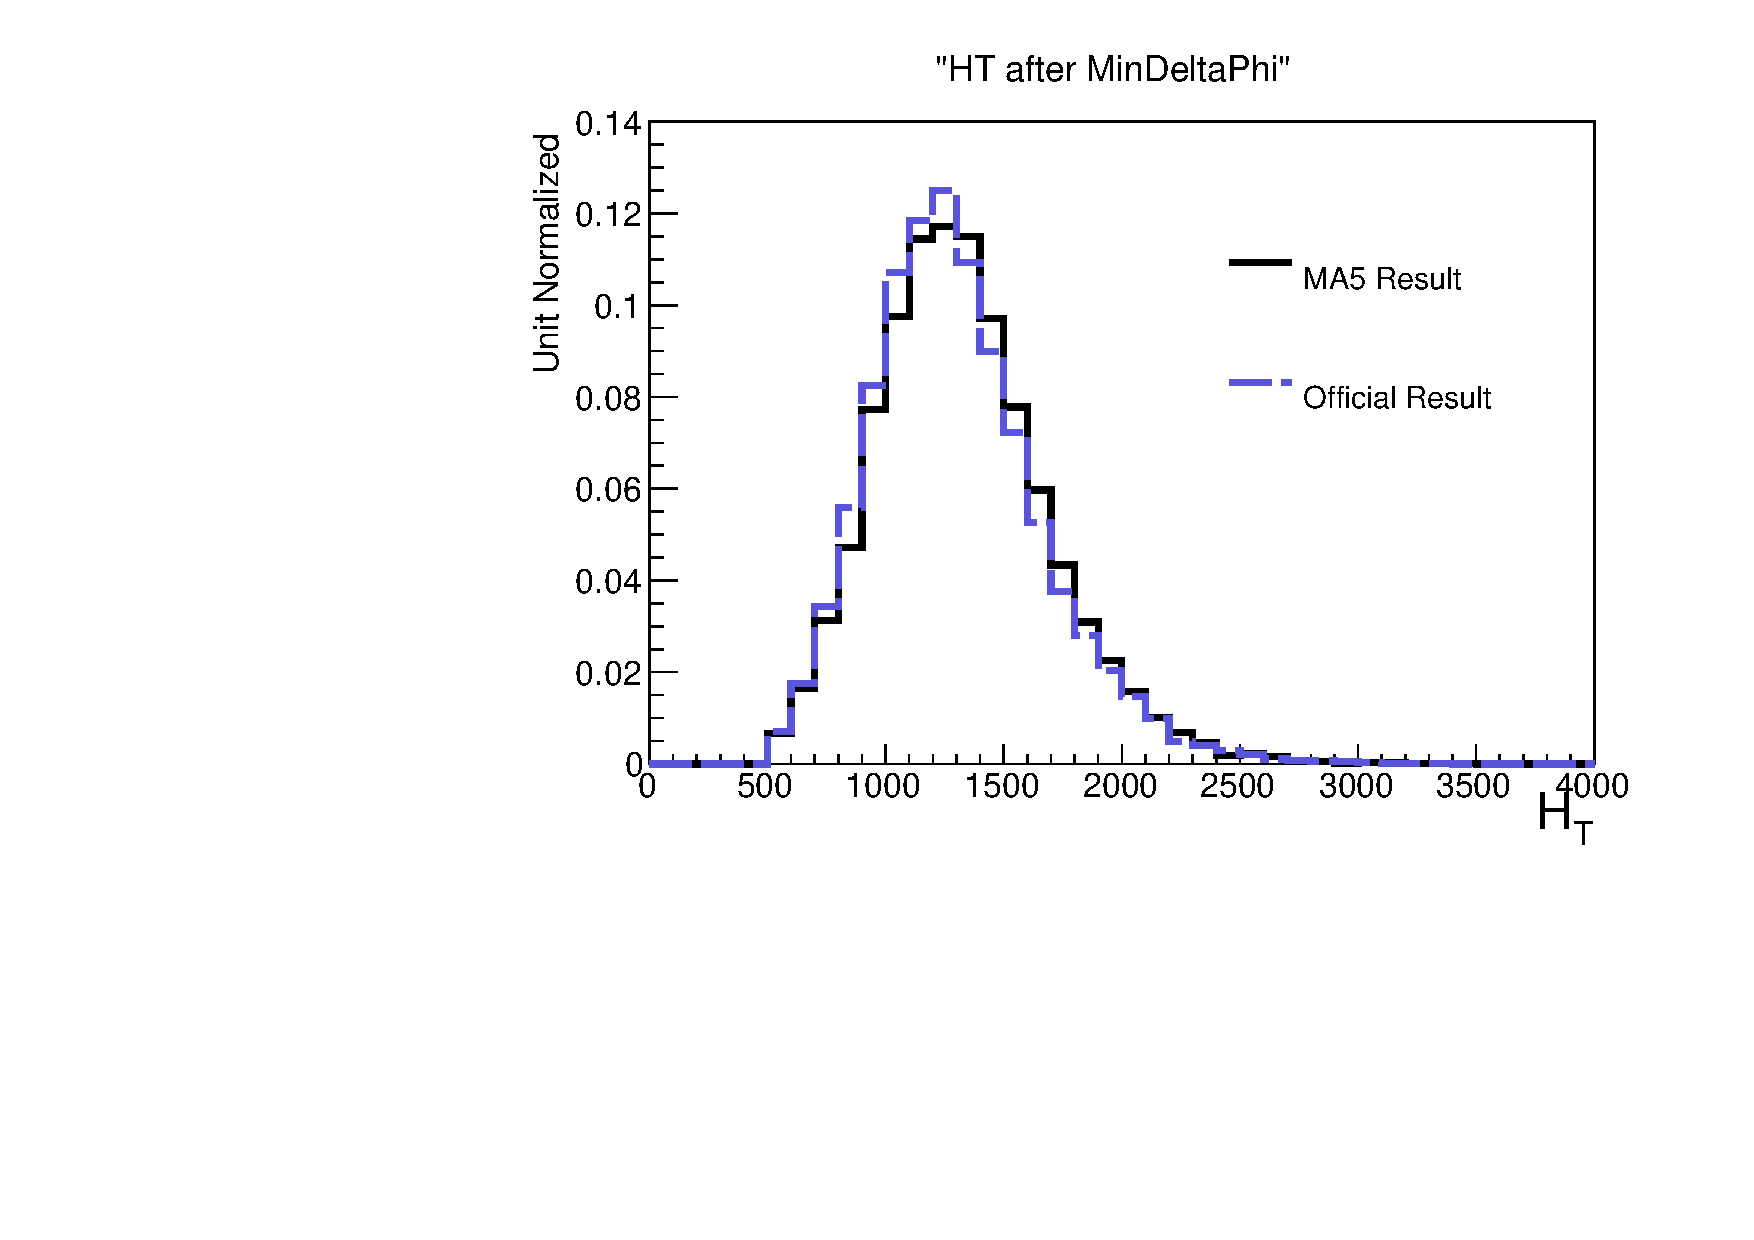
\includegraphics[width=0.5\textwidth]{figures/Appendices/Ma5ValidationSUS13012/T5VV_HT_after_MinDeltaPhi.pdf}
                \label{fig:tiger}
        }
        \caption{Comparison of the distributions of $H_T$ between the official and our own samples after the ``n-1" cut, Min $\Delta(\phi)$ (left), and after all baseline cuts (right), for the T5VV signal model.}\label{fig:animals}
\end{figure}        
        
\begin{figure}
        \centering
        \subfloat[]{
                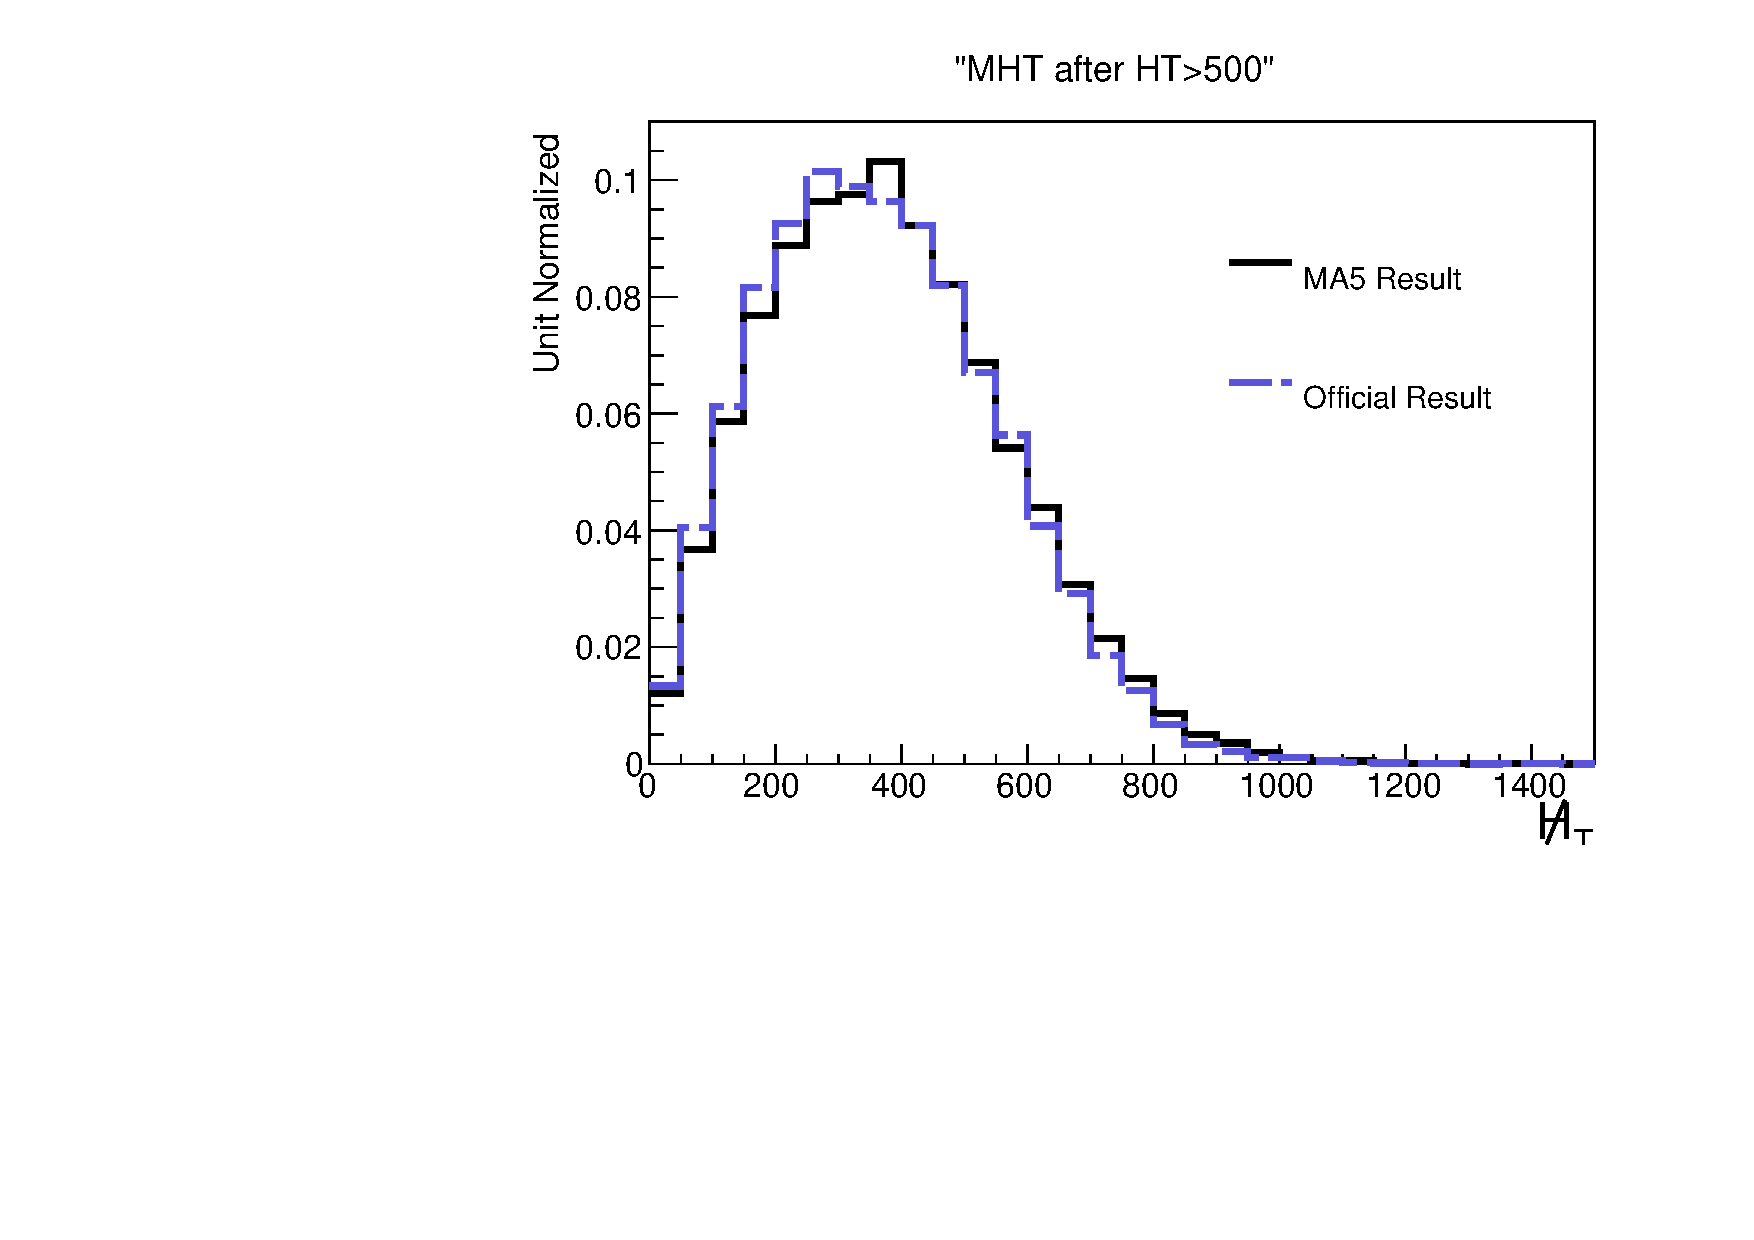
\includegraphics[width=0.5\textwidth]{figures/Appendices/Ma5ValidationSUS13012/T5VV_MHT_after_HT>500.pdf}
                \label{fig:gull}
        }%
        \hspace{-1 cm}
        ~ %add desired spacing between images, e. g. ~, \quad, \qquad, \hfill etc.
          %(or a blank line to force the subfigure onto a new line)
        \subfloat[]{
                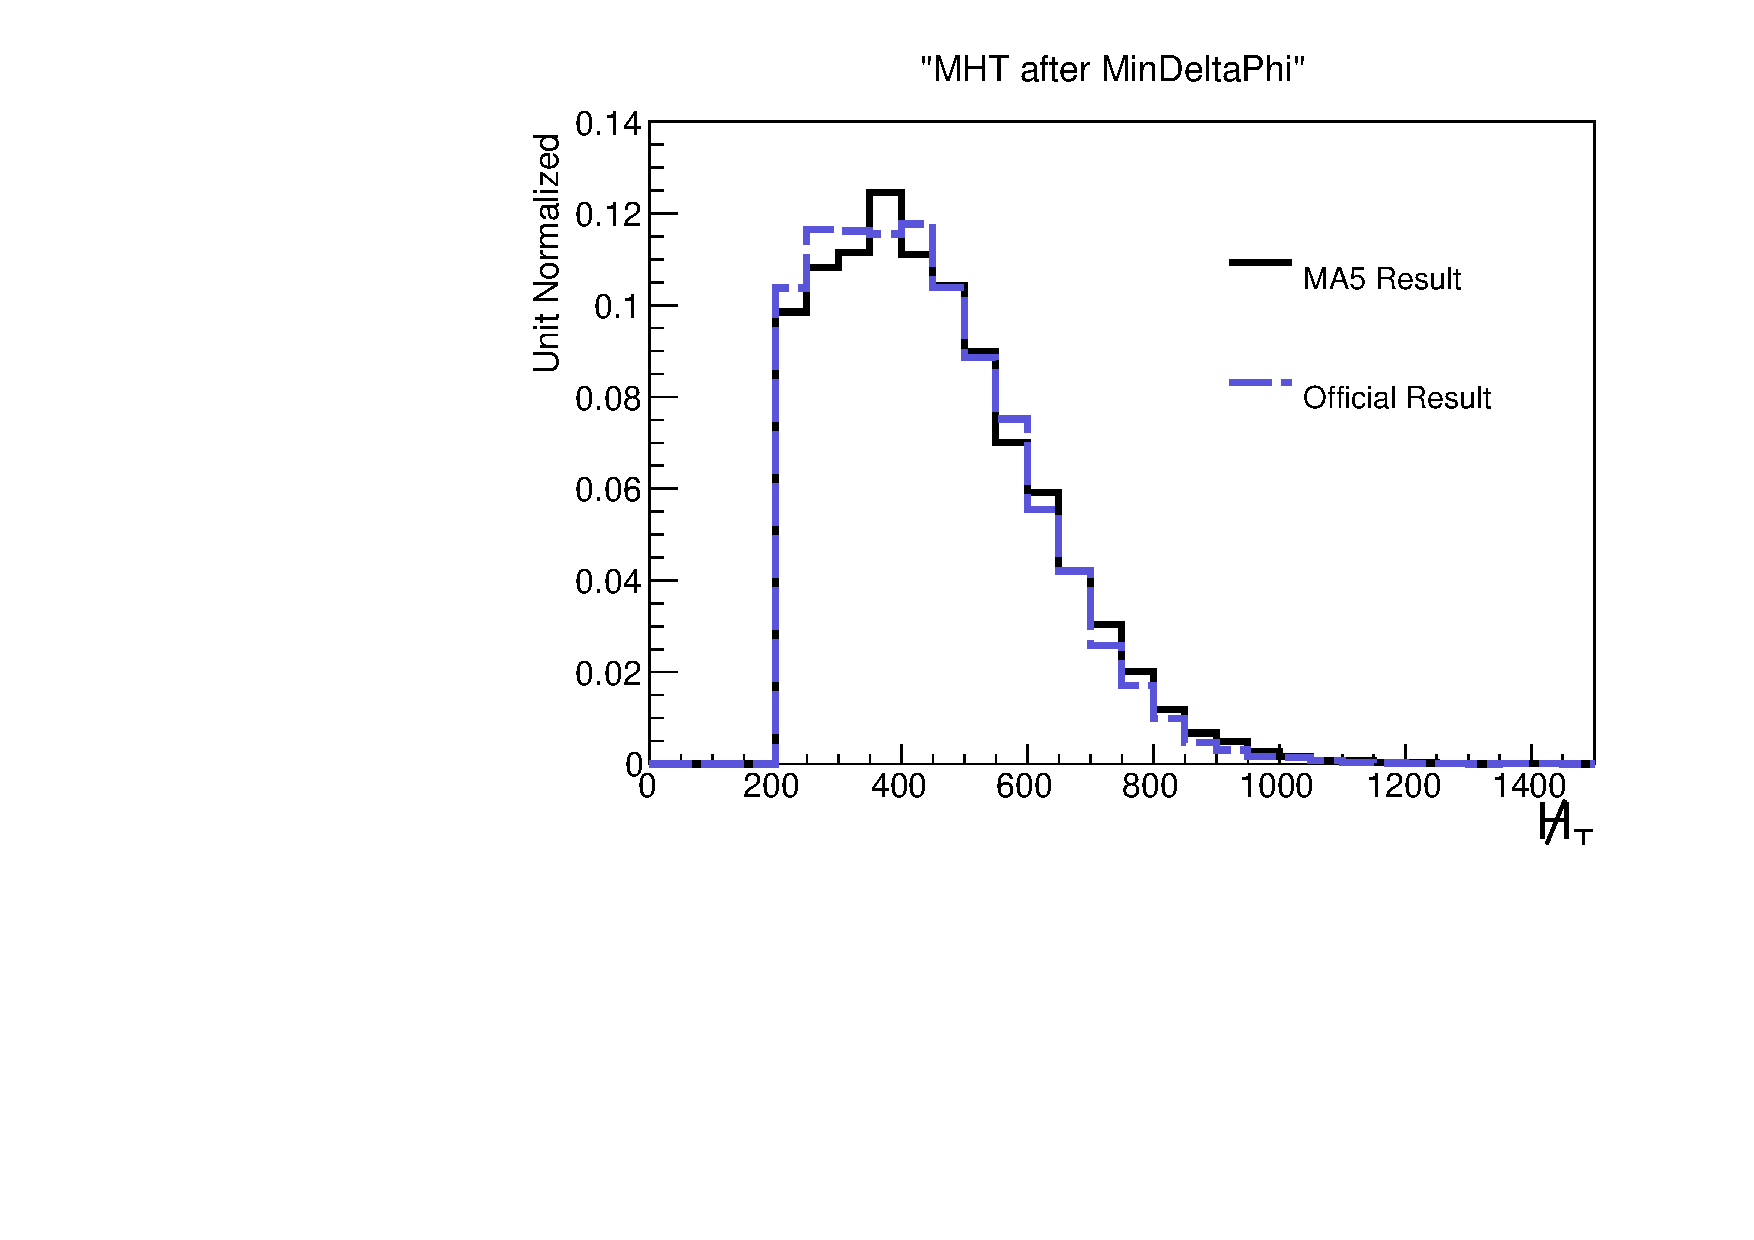
\includegraphics[width=0.5\textwidth]{figures/Appendices/Ma5ValidationSUS13012/T5VV_MHT_after_MinDeltaPhi.pdf}
                \label{fig:tiger}
        }
        \caption{Comparison of the distributions of \MHT between the official and our own samples after the ``n-1" cut, Min $\Delta(\phi)$ (left), and after all baseline cuts (right), for the T5VV signal model.}\label{fig:animals}
\end{figure}        
        
\begin{figure}
        \centering
        \subfloat[]{
                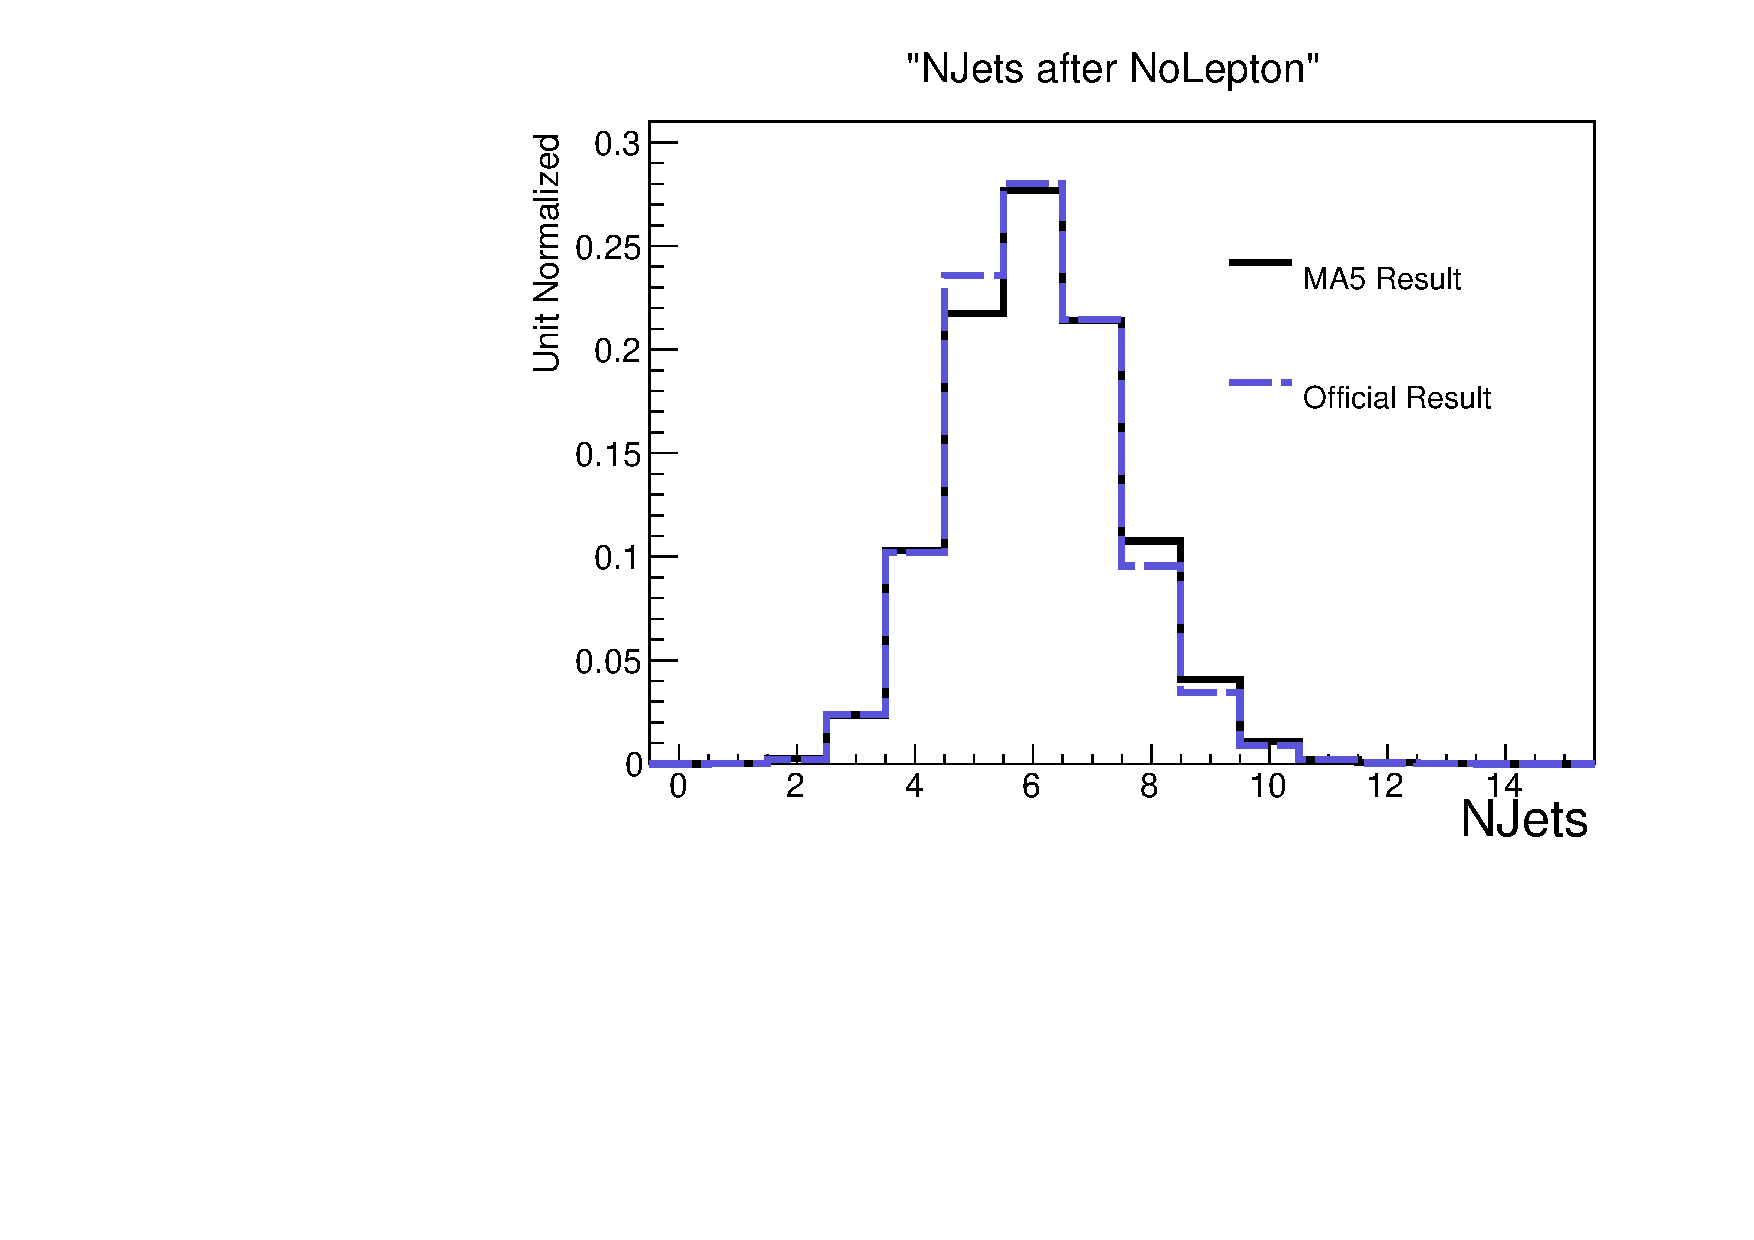
\includegraphics[width=0.5\textwidth]{figures/Appendices/Ma5ValidationSUS13012/T5VV_NJets_after_NoLepton.pdf}
                \label{fig:gull}
        }%
        \hspace{-1 cm}
        ~ %add desired spacing between images, e. g. ~, \quad, \qquad, \hfill etc.
          %(or a blank line to force the subfigure onto a new line)
        \subfloat[]{
                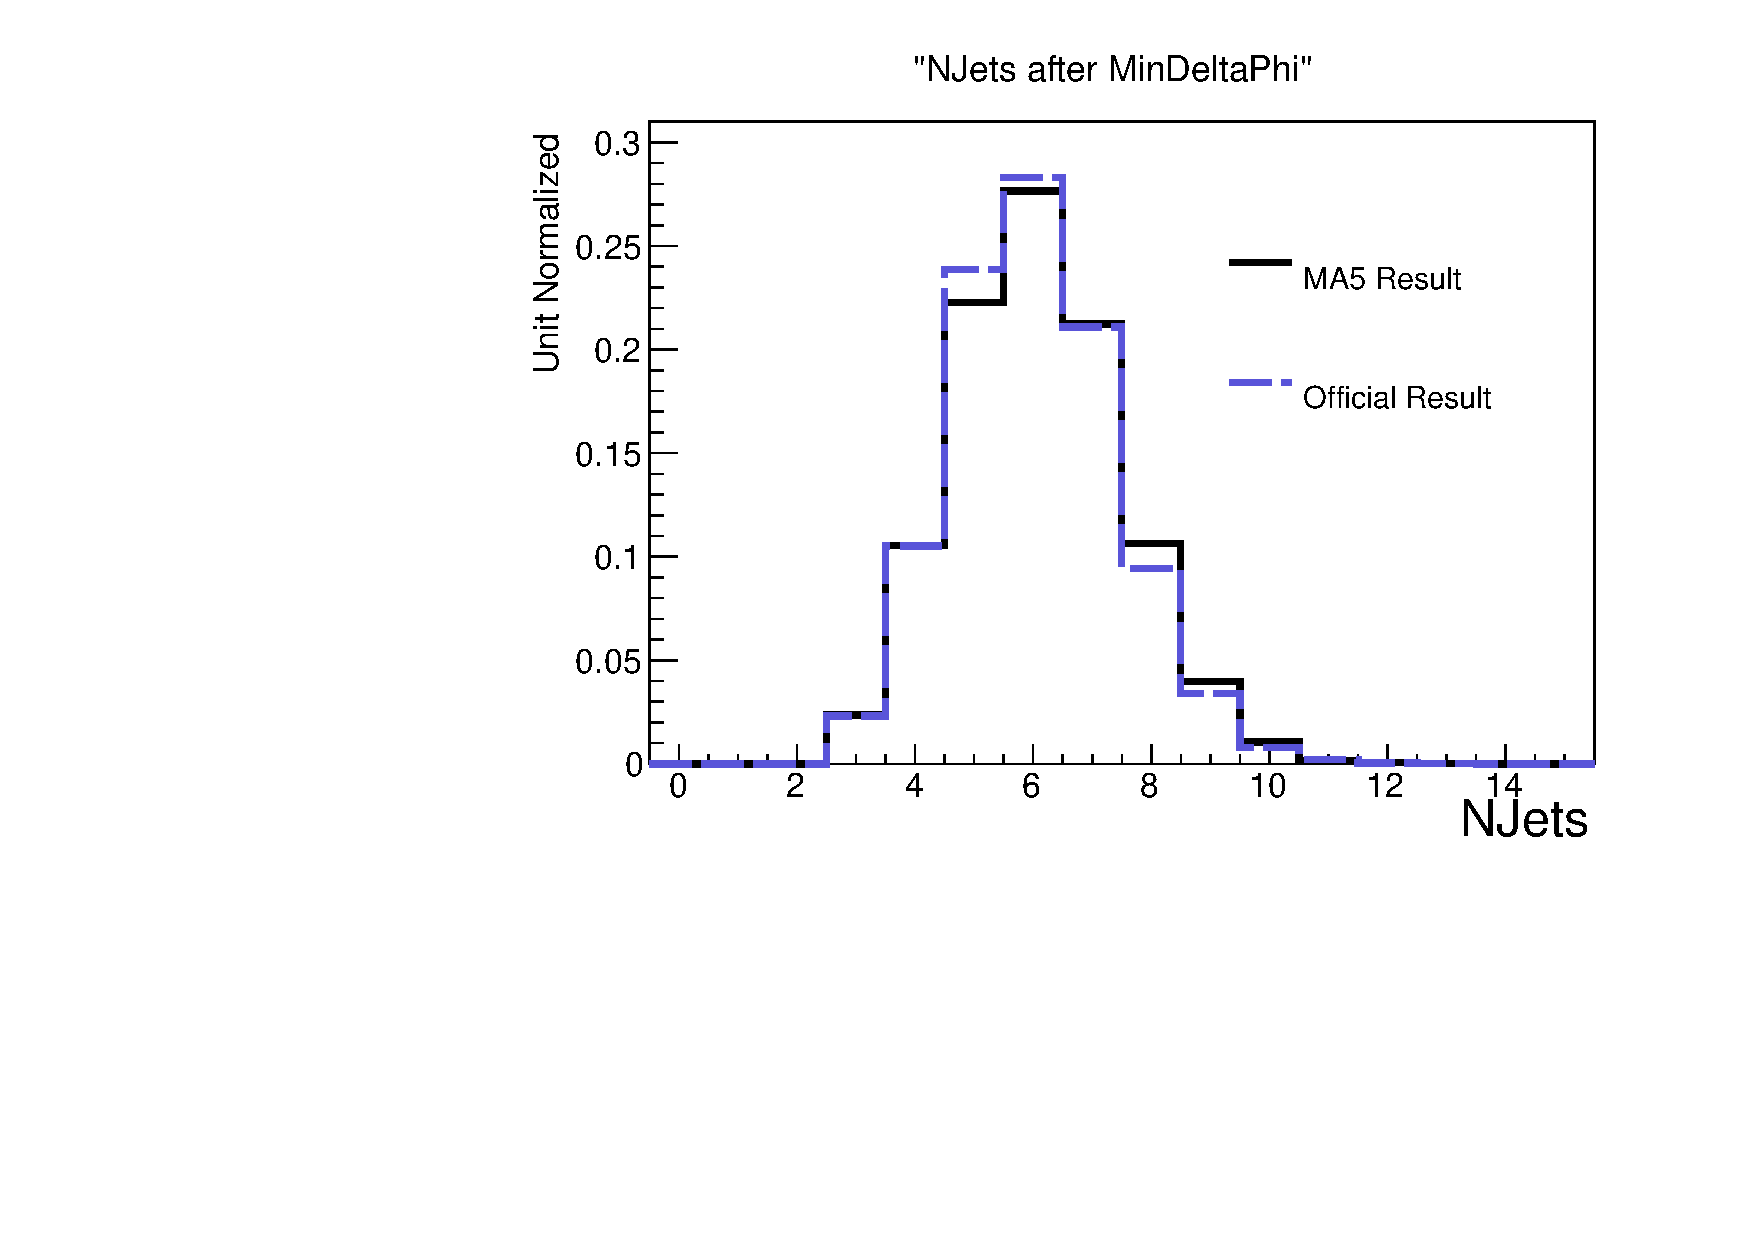
\includegraphics[width=0.5\textwidth]{figures/Appendices/Ma5ValidationSUS13012/T5VV_NJets_after_MinDeltaPhi.pdf}
                \label{fig:tiger}
        }
        \caption{Comparison of the distributions of NJets between the official and our own samples after the ``n-1" cut, Min $\Delta(\phi)$ (left), and after all baseline cuts (right), for the T5VV signal model.}\label{fig:animals}
\end{figure}        
        
        \begin{figure}
        \centering
        \subfloat[]{
        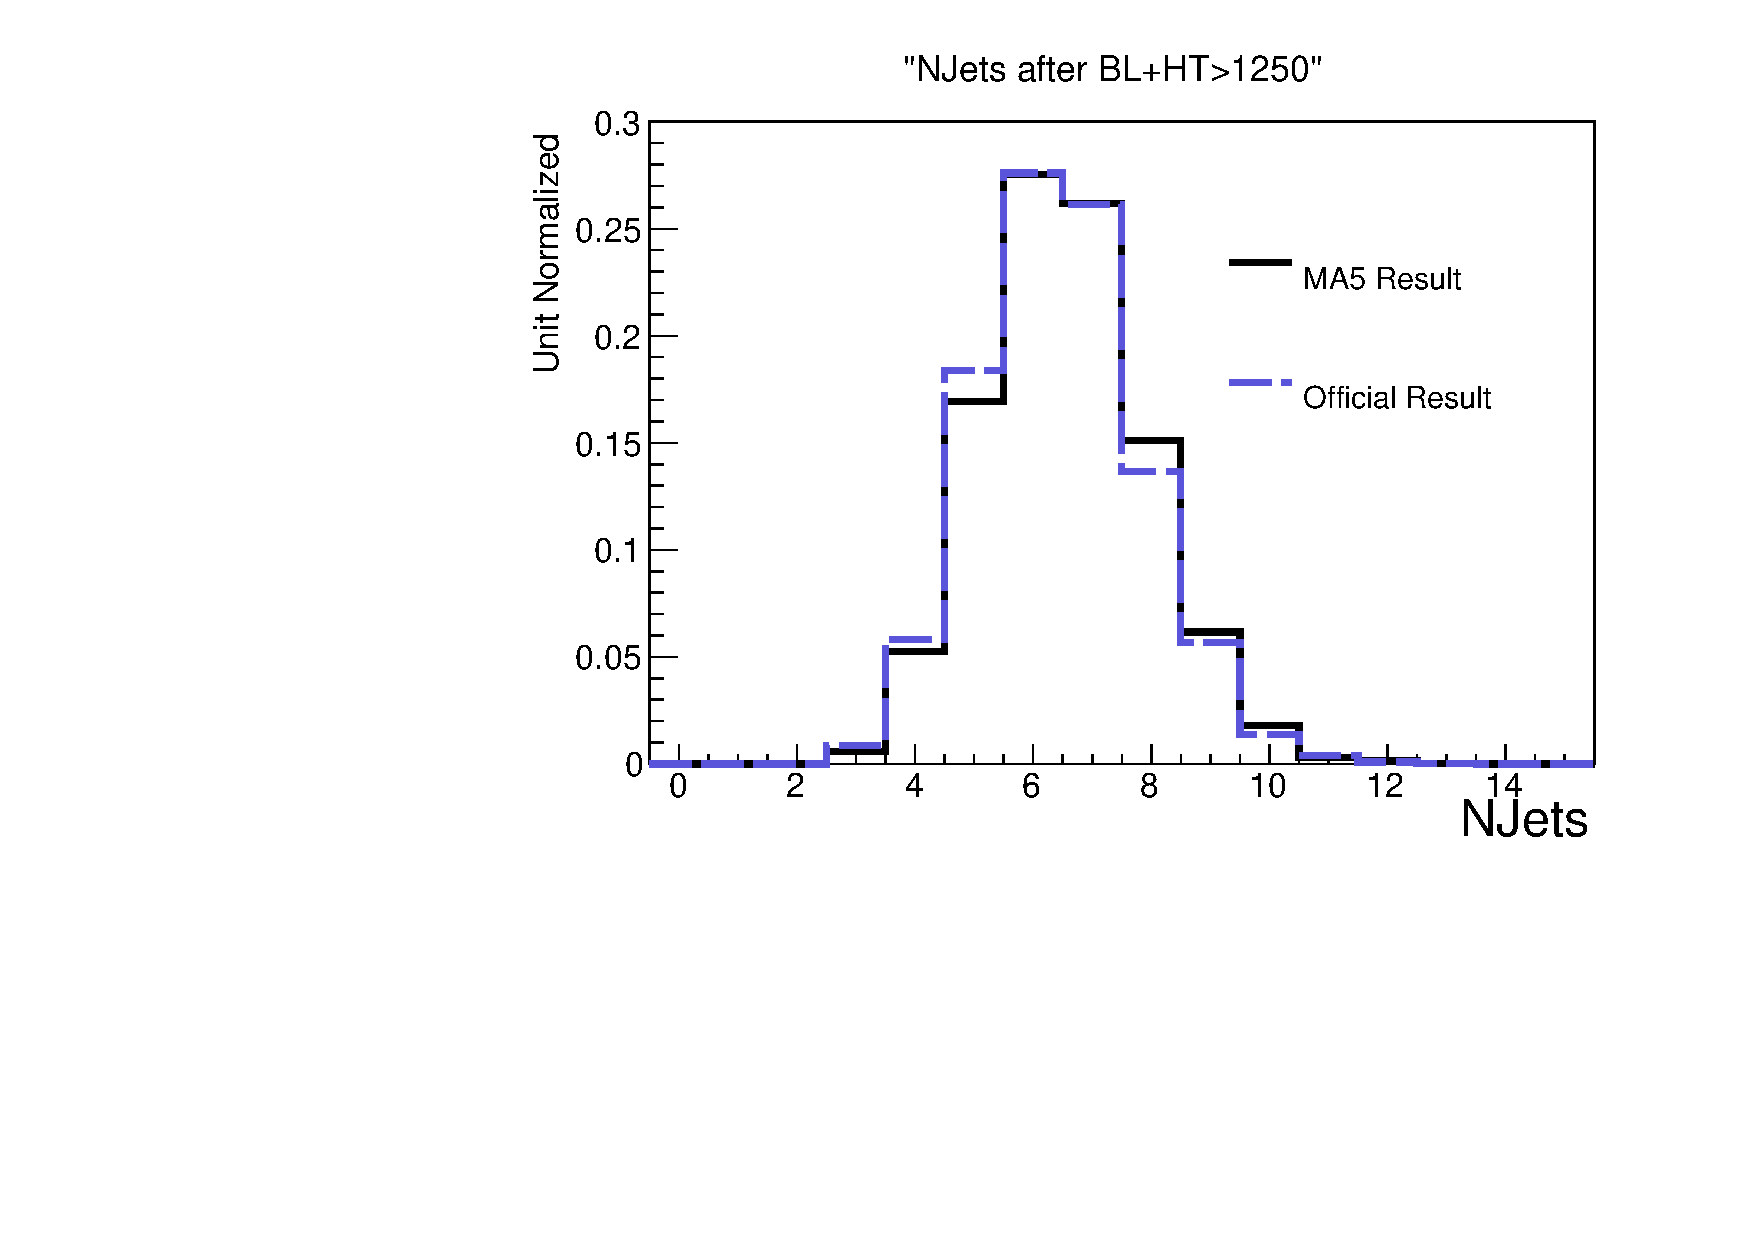
\includegraphics[width=0.5\textwidth]{figures/Appendices/Ma5ValidationSUS13012/T5VV_NJets_after_BL+HT>1250.pdf}
        \label{fig:gull}
        }%
        \hspace{-1 cm}
        ~ %add desired spacing between images, e. g. ~, \quad, \qquad, \hfill etc.
        %(or a blank line to force the subfigure onto a new line)
        \subfloat[]{
        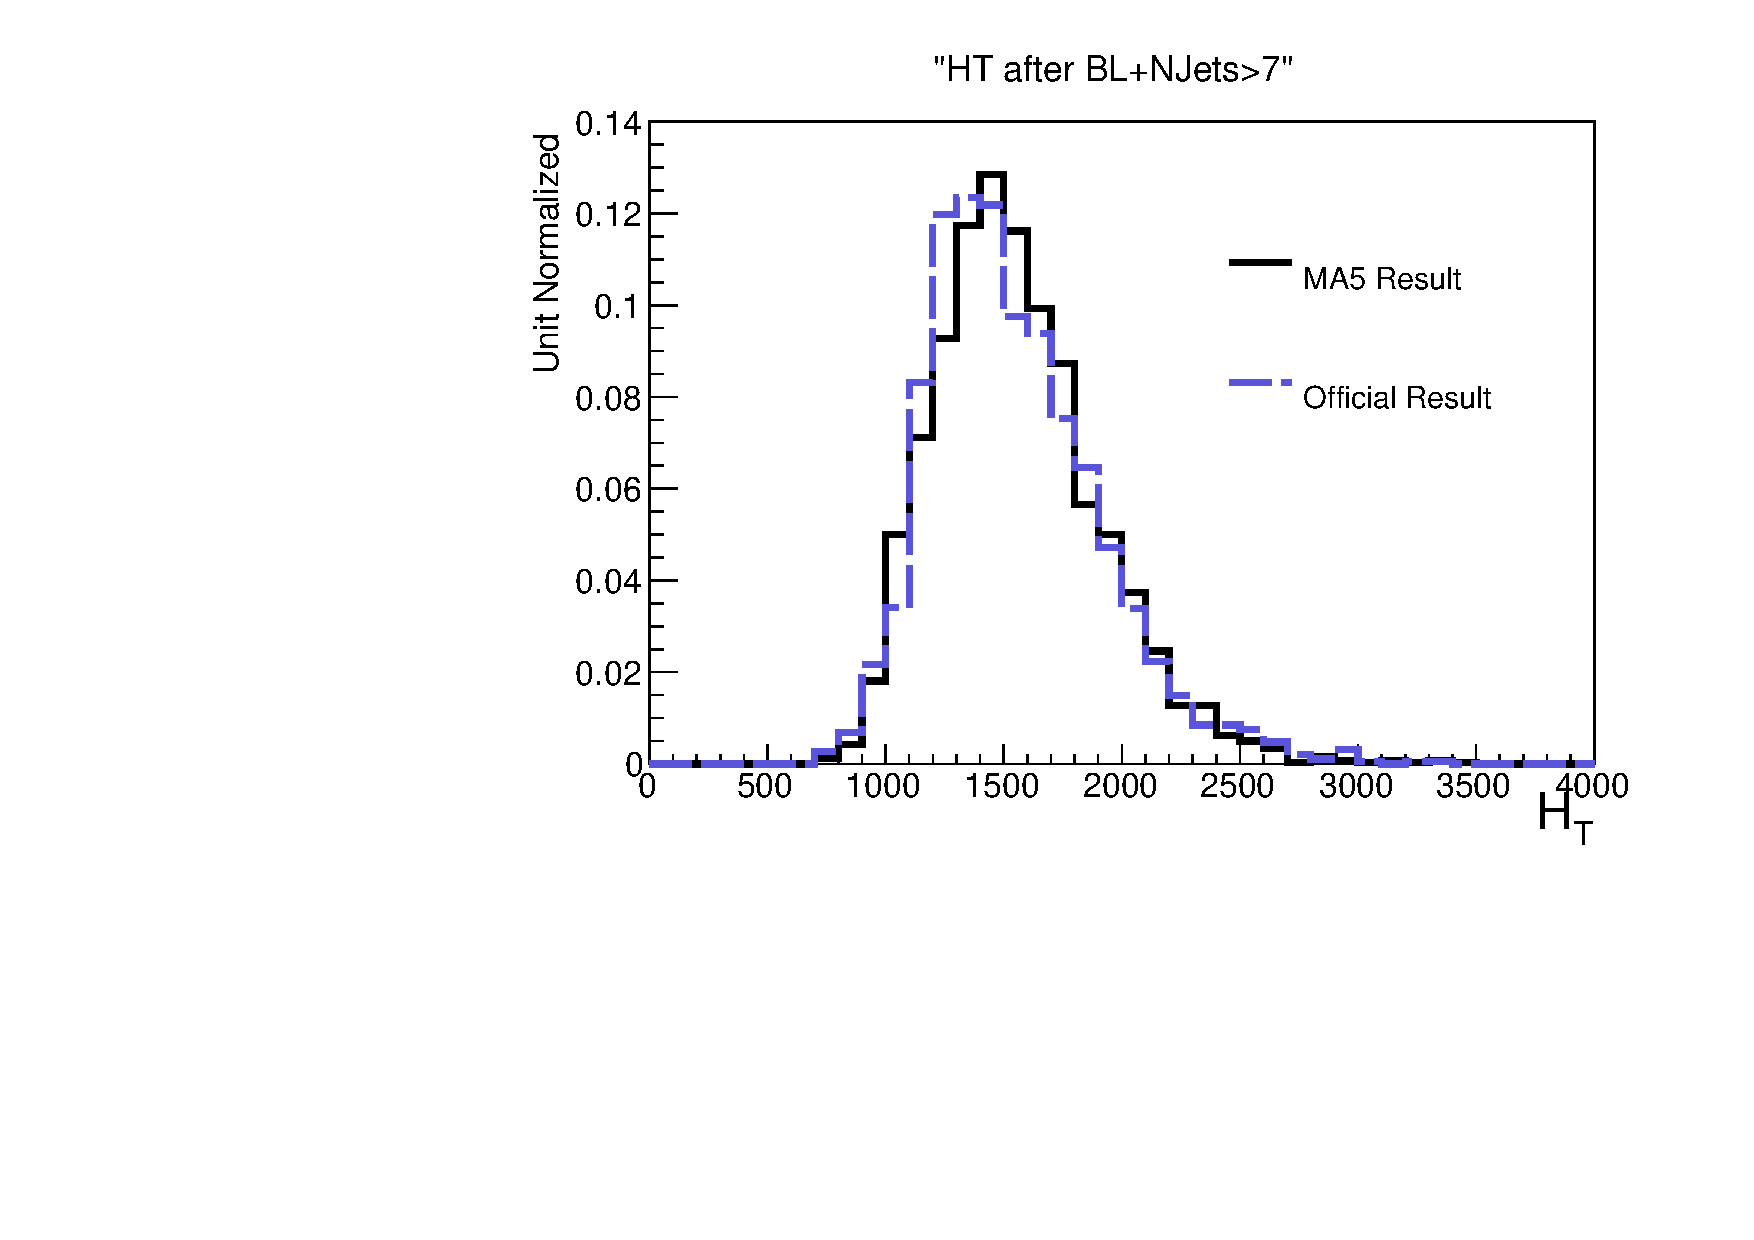
\includegraphics[width=0.5\textwidth]{figures/Appendices/Ma5ValidationSUS13012/T5VV_HT_after_BL+NJets>7.pdf}
        \label{fig:tiger}
        }
        \caption{Additional checks: comparison between ours and the official distributions of NJets after BL+$H_T$$>$1250 cuts (left), and $H_T$ after BL+NJets$>$7 cuts (right), for the T5VV signal model.}
        \end{figure}   
        

\clearpage
%%%%%%%%%%%%%%%%%%%%%%%%%%%%%%%%%%%%%%%%%%%%%%%%%
\subsection{T2qq simplified model}
%%%%%%%%%%%%%%%%%%%%%%%%%%%%%%%%%%%%%%%%%%%%%%%%%

\begin{figure}[h!]
\centering
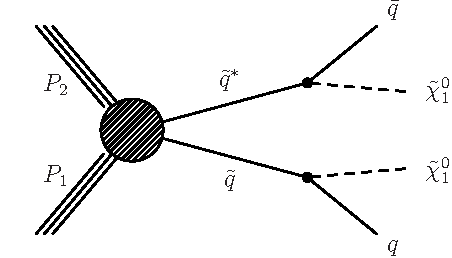
\includegraphics[width=7cm]{figures/Appendices/Ma5ValidationSUS13012/T2qq.pdf}
\caption{Diagram of the dominant SUSY production mechanism
for the T2qq signal model.}
\label{fig:T2qq}
\end{figure}

    \begin{table}[h!]
    \begin{centering}
    \begin{tabular}{  c | c | c  }
    \hline
    \hline
    Cut Name & Official Count (Eff) & MA5 Count (Eff)\\
    \hline
        MET Cleaning & 1215.2 (xxx) & 1215.2 (xxx)\\
    No Lepton & 1212.8 (99\%) & 1215.2 (100\%)\\
    NJets$>$2 & 675.9 (55\%) & 691.54 (56\%)\\
    $H_T$$>$500 & 619.5 (91\%) & 638.41 (92\%)\\
    \MHT$>$200 & 524.0 (84\%) & 539.59 (84\%)\\
    Min $\Delta(\phi)$ & 460.7 (87\%) & 476.12 (88\%)\\
\hline
\hline
    \end{tabular}
    \caption{The cut flow for the baseline selection in CMS SUS-13-012 for
    the T2qq  working point  $(m_{\tilde q},\,m_{\tilde\chi^0_1})=(700,\,100)$~GeV. 
    The second column is the official account as
    reported by
    https://twiki.cern.ch/twiki/pub/CMSPublic/PhysicsResultsSUS13012/T2qq.pdf,
    and our own results are given in column 3. The official counts are
    normalized to luminosity ${\cal L}=19.5$/fb and cross section $\sigma= 63.4$~pb, and our
    counts are normalized to match the official count after the first cut, MET
    Cleaning.}
    \label{table:CF4}
    \end{centering}
    \end{table}
    
    \begin{table}
    \begin{centering}
    \begin{tabular}{  l | c | c  }
    \hline
    \hline
    Signal Region Name & Official & MA5\\
    \hline
    NJets3-5,  $H_T$500-800,  \MHT200-300 & 35.3 & 35.10\\ 
 \hline 
NJets3-5,  $H_T$500-800,  \MHT300-450 & 70.4 & 73.44\\ 
 \hline 
NJets3-5,  $H_T$500-800,  \MHT450-600 & 71.5 & 73.82\\ 
 \hline 
NJets3-5,  $H_T$500-800,  \MHT$>$600 & 23.6 & 28.78\\ 
 \hline 
NJets3-5,  $H_T$800-1000,  \MHT200-300 & 18.1 & 17.20\\ 
 \hline 
NJets3-5,  $H_T$800-1000,  \MHT300-450 & 21.9 & 32.19\\ 
 \hline 
NJets3-5,  $H_T$800-1000,  \MHT450-600 & 38.1 & 38.14\\ 
 \hline 
NJets3-5,  $H_T$800-1000,  \MHT$>$600 & 35.2 & 36.74\\ 
 \hline 
NJets3-5,  $H_T$1000-1250,  \MHT200-300 & 10.9 & 12.15\\ 
 \hline 
NJets3-5,  $H_T$1000-1250,  \MHT300-450 & 21.7 & 20.31\\ 
 \hline 
NJets3-5,  $H_T$1000-1250,  \MHT450-600 & 20.7 & 21.54\\ 
 \hline 
NJets3-5,  $H_T$1000-1250,  \MHT$>$600 & 21.8 & 23.59\\ 
 \hline 
NJets3-5,  $H_T$1250-1500,  \MHT200-300 & 4.3 & 5.53\\ 
 \hline 
NJets3-5,  $H_T$1250-1500,  \MHT300-450 & 8.1 & 7.85\\ 
 \hline 
NJets3-5,  $H_T$1250-1500,  \MHT$>$450 & 16.1 & 16.86\\ 
 \hline 
NJets3-5,  $H_T$$>$1500,  \MHT200-300 & 3.7 & 3.68\\ 
 \hline 
NJets3-5,  $H_T$$>$1500,  \MHT$>$300 & 13. & 13.45\\ 
 \hline 
NJets6-7,  $H_T$500-800,  \MHT200-300 & 0.8 & 0.40\\ 
 \hline 
NJets6-7,  $H_T$500-800,  \MHT300-450 & 1.0 & 0.44\\ 
 \hline 
NJets6-7,  $H_T$500-800,  \MHT$>$450 & 0.4 & 0.44\\ 
 \hline 
NJets6-7,  $H_T$800-1000,  \MHT200-300 & 0.5 & 0.58\\ 
 \hline 
NJets6-7,  $H_T$800-1000,  \MHT300-450 & 1.1 & 1.26\\ 
 \hline 
NJets6-7,  $H_T$800-1000,  \MHT$>$450 & 1.5 & 1.63\\ 
 \hline 
NJets6-7,  $H_T$1000-1250,  \MHT200-300 & 1.0 & 0.61\\ 
 \hline 
NJets6-7,  $H_T$1000-1250,  \MHT300-450 & 1.2 & 1.33\\ 
 \hline 
NJets6-7,  $H_T$1000-1250,  \MHT$>$450 & 2.5 & 3.24\\ 
 \hline 
NJets6-7,  $H_T$1250-1500,  \MHT200-300 & 0.6 & 0.61\\ 
 \hline 
NJets6-7,  $H_T$1250-1500,  \MHT300-450 & 1.2 & 0.61\\ 
 \hline 
NJets6-7,  $H_T$1250-1500,  \MHT$>$450 & 1.4 & 1.84\\ 
 \hline 
NJets6-7,  $H_T$$>$1500,  \MHT200-300 & 0.6 & 0.30\\ 
 \hline 
NJets6-7,  $H_T$$>$1500,  \MHT$>$300 & 2.3 & 1.80\\ 
 \hline 
NJets$>$7,  $H_T$500-800,  \MHT$>$200 & 0.0 & 0.0\\ 
 \hline 
NJets$>$7,  $H_T$800-1000,  \MHT$>$200 & 0.0 & 0.0\\ 
 \hline 
NJets$>$7,  $H_T$1000-1250,  \MHT$>$200 & 0.2 & 0.27\\ 
 \hline 
NJets$>$7,  $H_T$1250-1500,  \MHT$>$200 & 0.3 & 0.10\\ 
 \hline 
NJets$>$7,  $H_T$$>$1500,  \MHT$>$200 & 0.3 & 0.13\\ 
 \hline 
\hline
    \end{tabular}
    \caption{The signal region (SR) counts in CMS SUS-13-012 for the T2qq scenario 
    after all selection has been applied. Column 2 is the official account obtained through generous correspondence with Christian Sanders,
    and our own results displayed in column 3. These counts were determined by applying the SR selection to the end of the cut flow featured in table \ref{table:CF4}.}
    \label{table:last}
    \end{centering}
    \end{table}
    
\begin{figure}
        \centering
        \subfloat[]{
                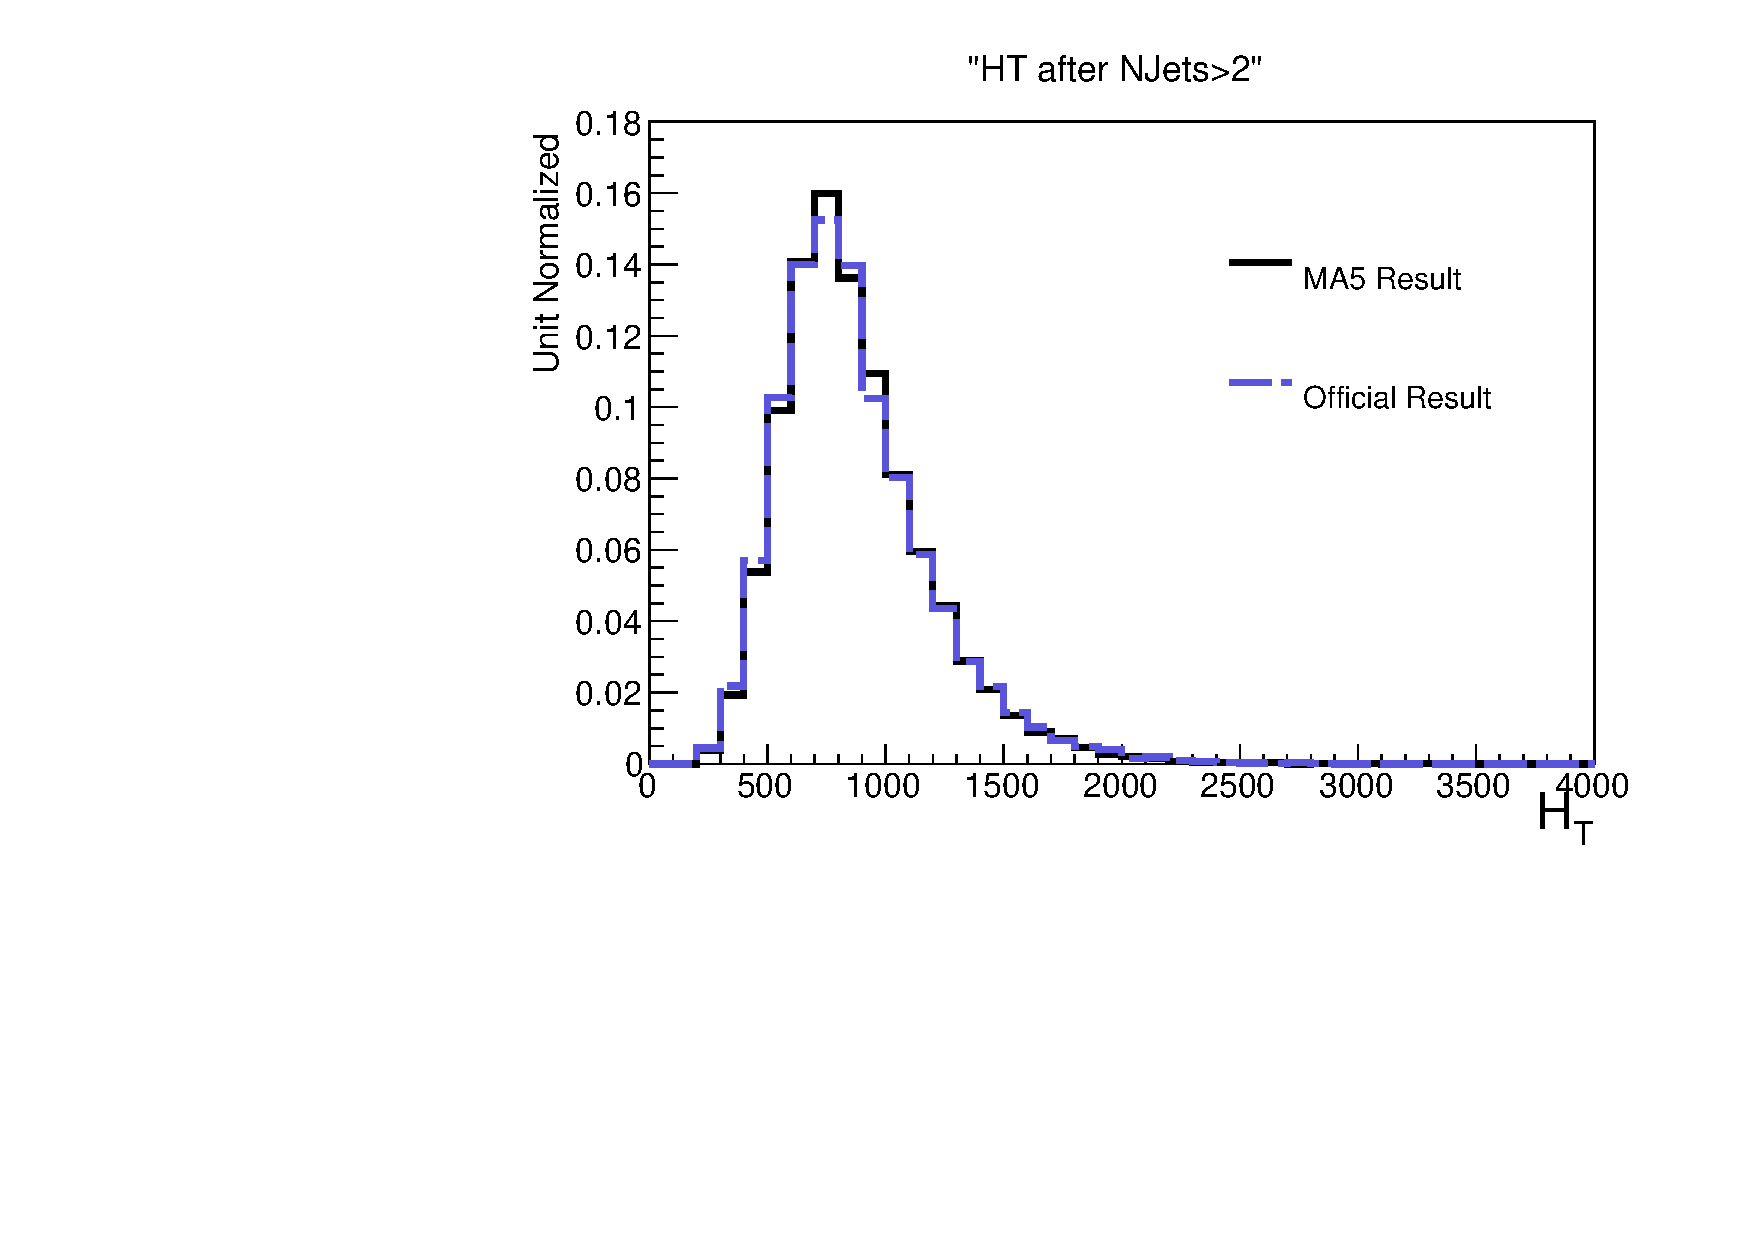
\includegraphics[width=0.5\textwidth]{figures/Appendices/Ma5ValidationSUS13012/T2qq_HT_after_NJets>2.pdf}
                \label{fig:gull}
        }%
        \hspace{-1 cm}
        ~ %add desired spacing between images, e. g. ~, \quad, \qquad, \hfill etc.
          %(or a blank line to force the subfigure onto a new line)
        \subfloat[]{
                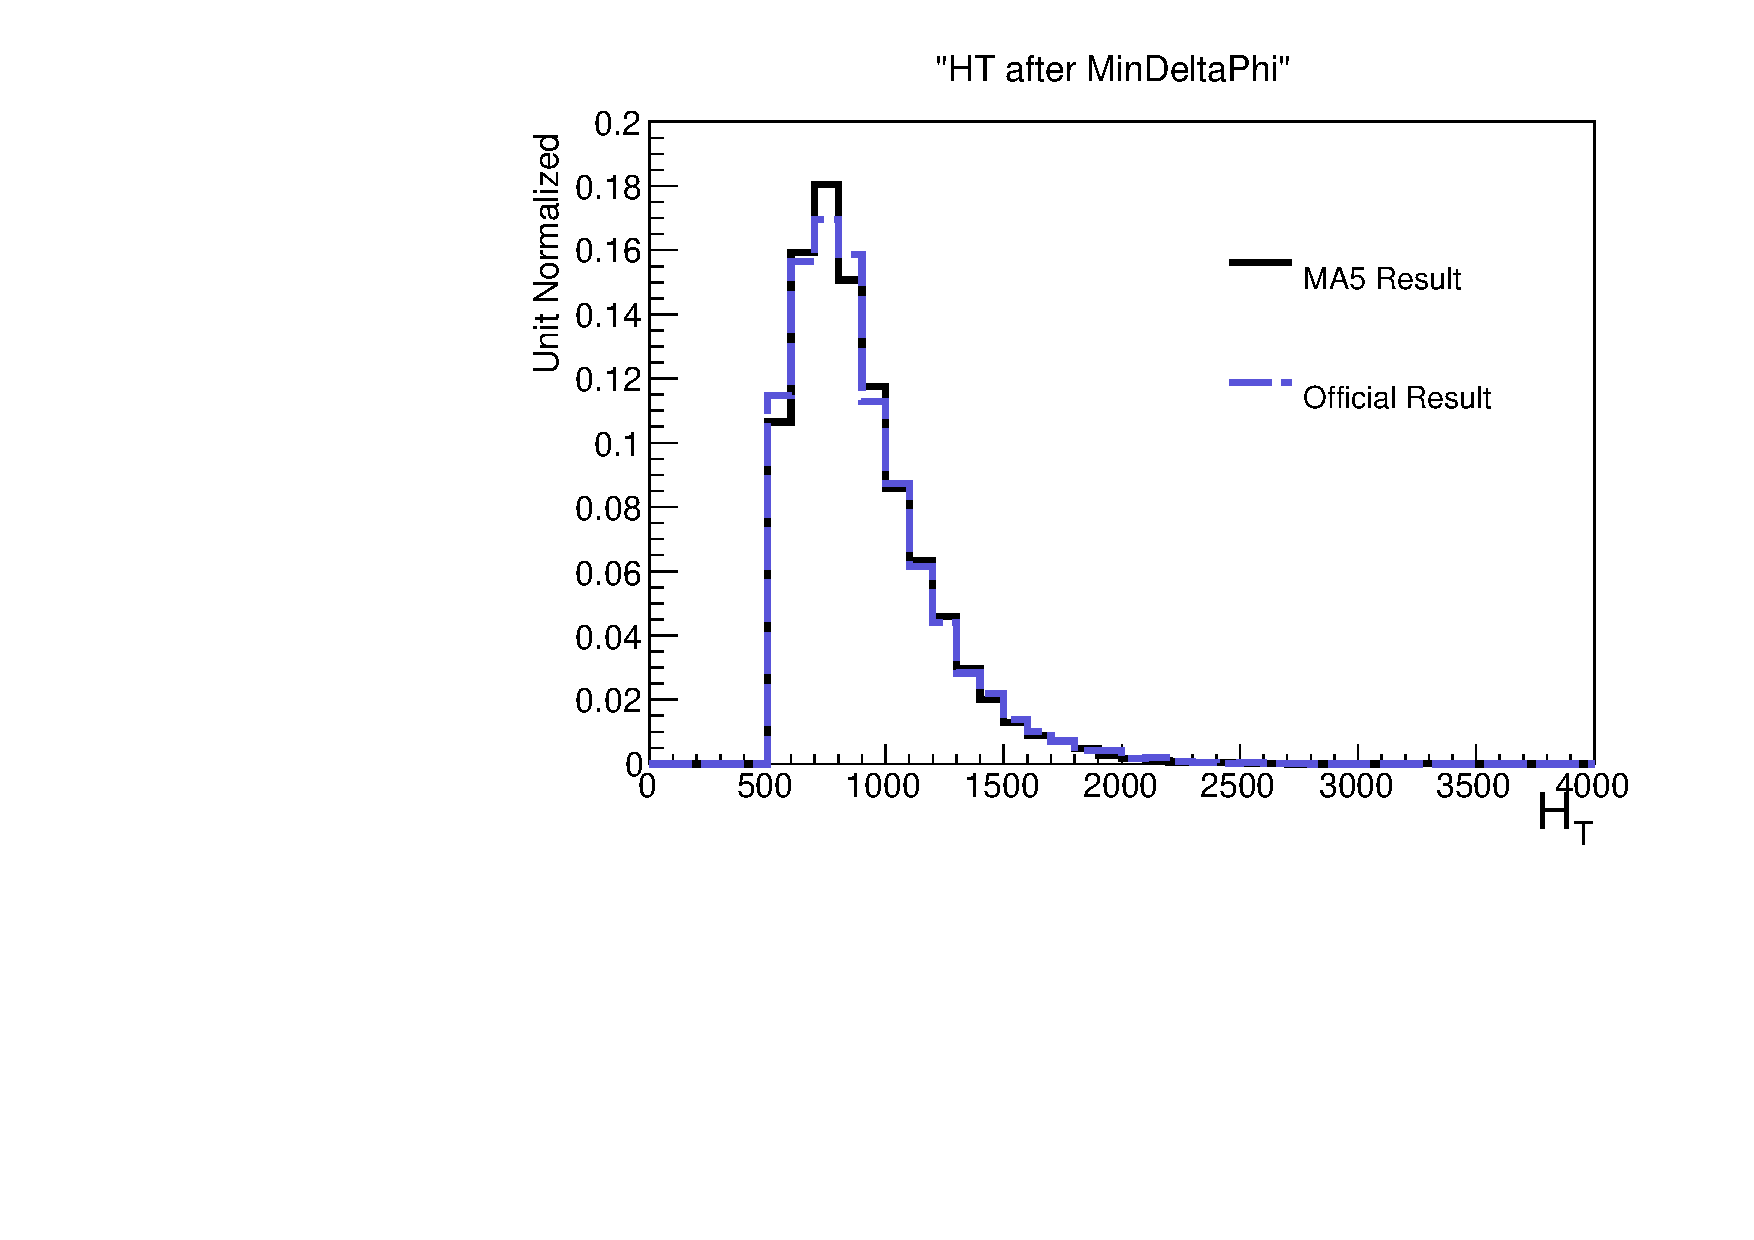
\includegraphics[width=0.5\textwidth]{figures/Appendices/Ma5ValidationSUS13012/T2qq_HT_after_MinDeltaPhi.pdf}
                \label{fig:tiger}
        }
        \caption{Comparison of the distributions of $H_T$ between the official and our own samples after the ``n-1" cut, Min $\Delta(\phi)$ (left), and after all baseline cuts (right), for the T2qq signal model.}\label{fig:animals}
\end{figure}        
        
\begin{figure}
        \centering
        \subfloat[]{
                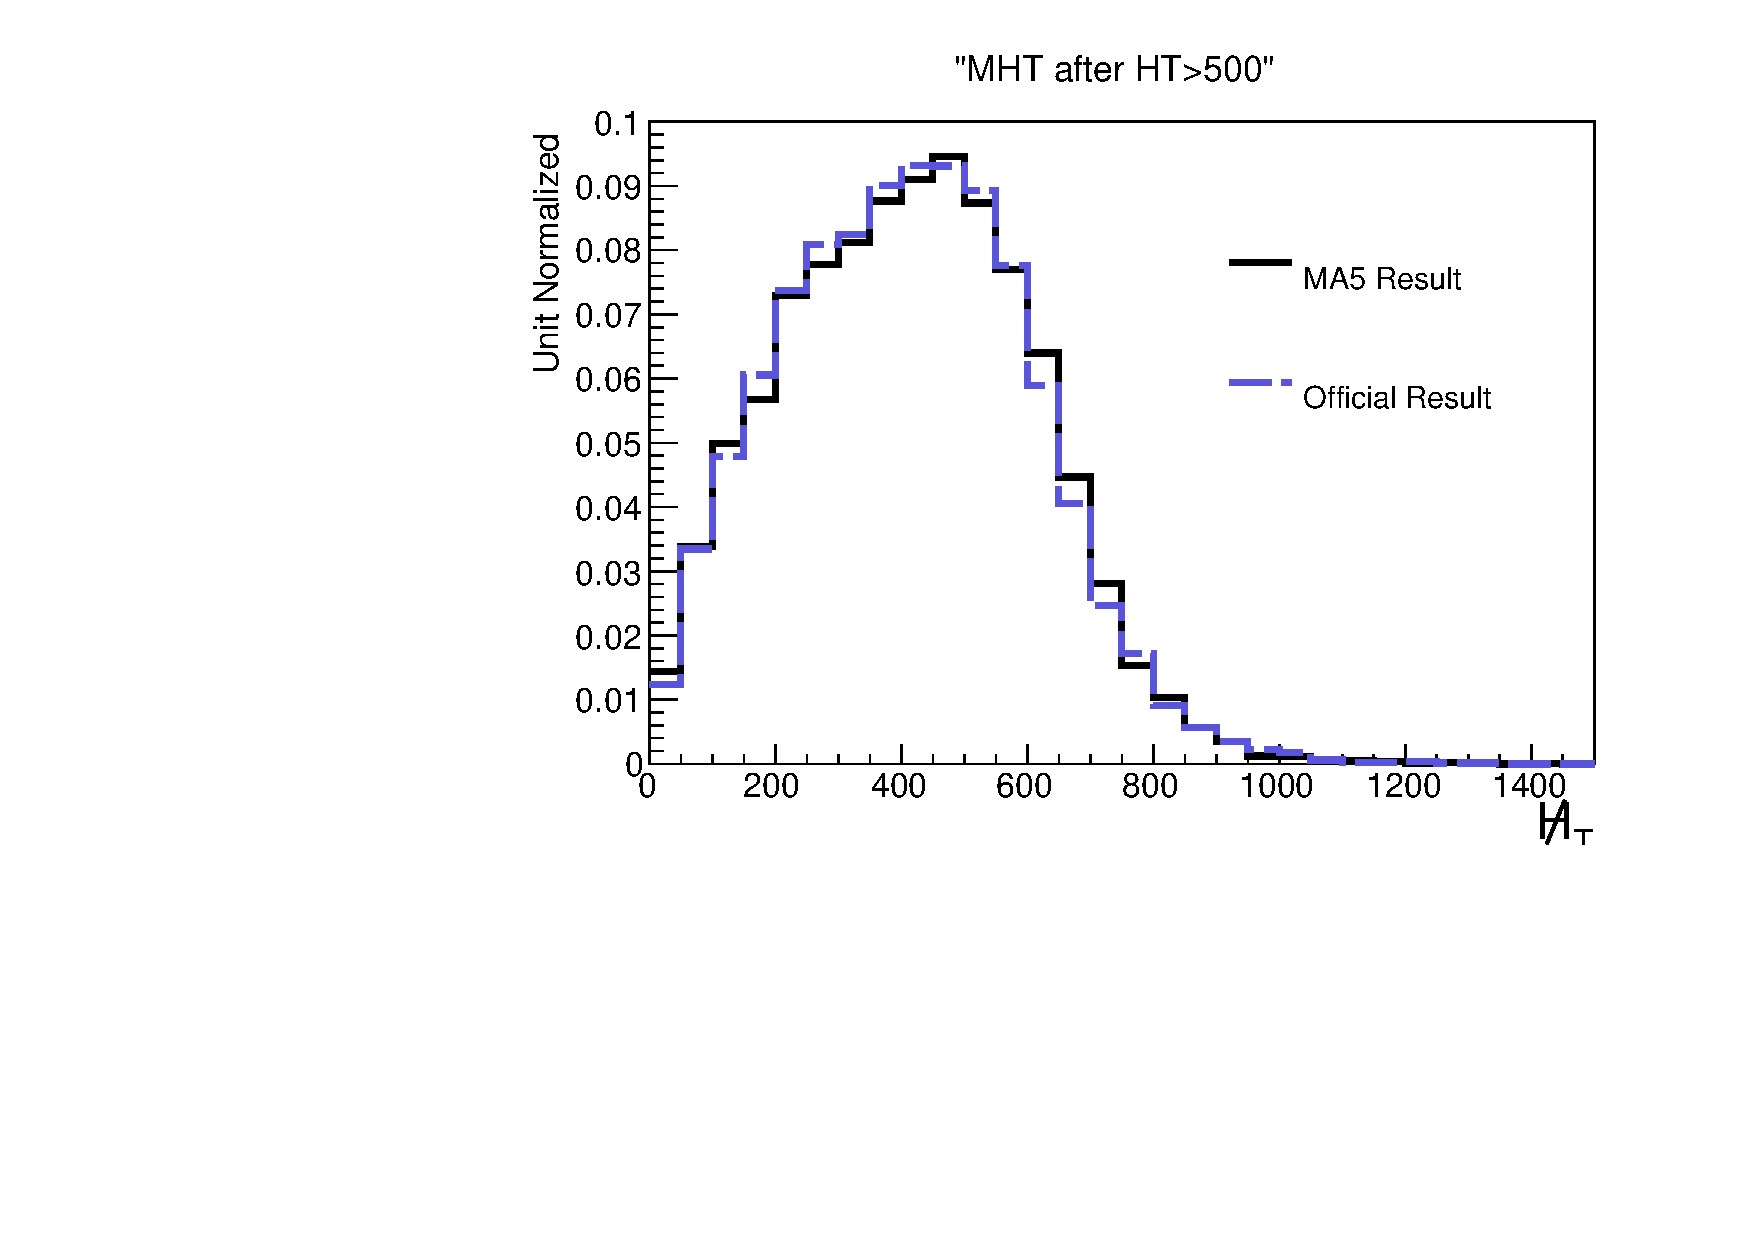
\includegraphics[width=0.5\textwidth]{figures/Appendices/Ma5ValidationSUS13012/T2qq_MHT_after_HT>500.pdf}
                \label{fig:gull}
        }%
        \hspace{-1 cm}
        ~ %add desired spacing between images, e. g. ~, \quad, \qquad, \hfill etc.
          %(or a blank line to force the subfigure onto a new line)
        \subfloat[]{
                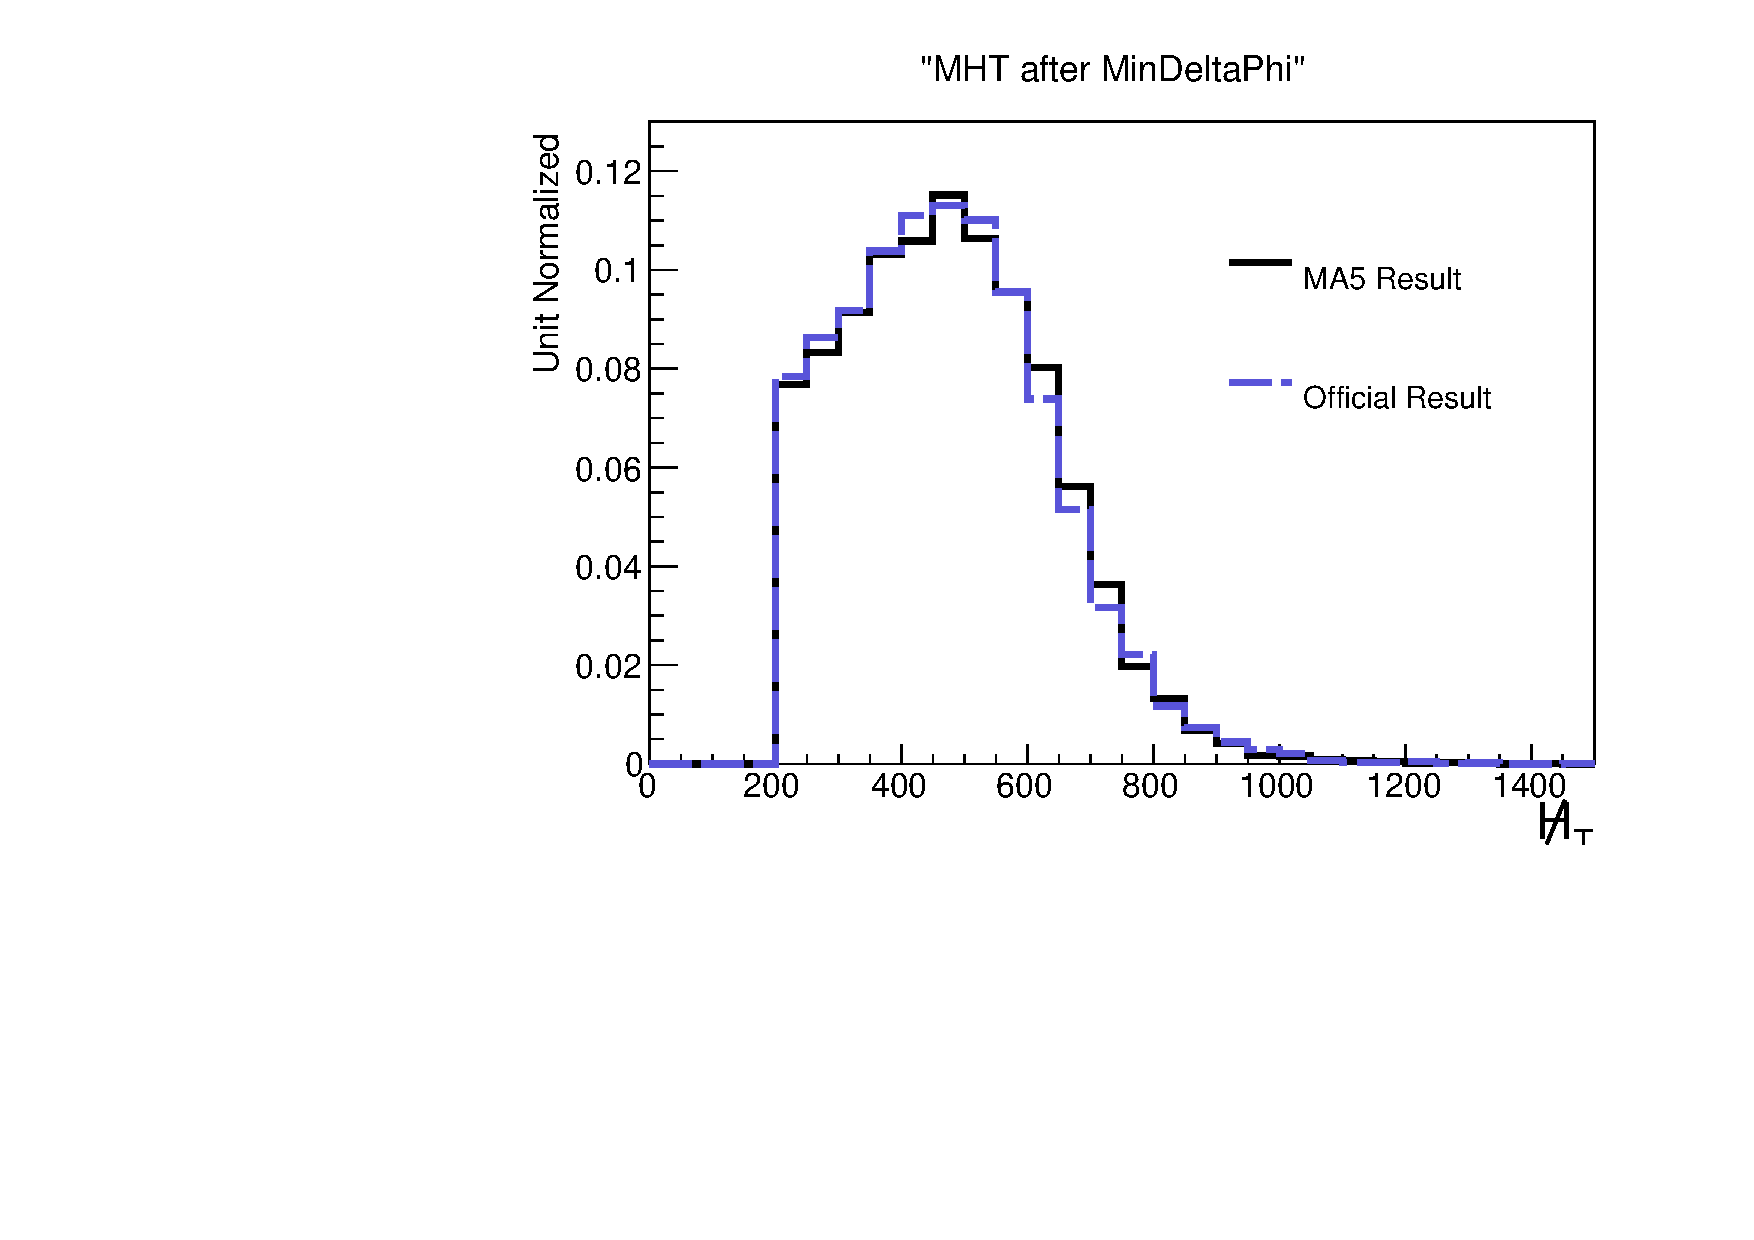
\includegraphics[width=0.5\textwidth]{figures/Appendices/Ma5ValidationSUS13012/T2qq_MHT_after_MinDeltaPhi.pdf}
                \label{fig:tiger}
        }
        \caption{Comparison of the distributions of \MHT between the official and our own samples after the ``n-1" cut, Min $\Delta(\phi)$ (left), and after all baseline cuts (right), for the T2qq signal model.}\label{fig:animals}
\end{figure}        
        
\begin{figure}
        \centering
        \subfloat[]{
                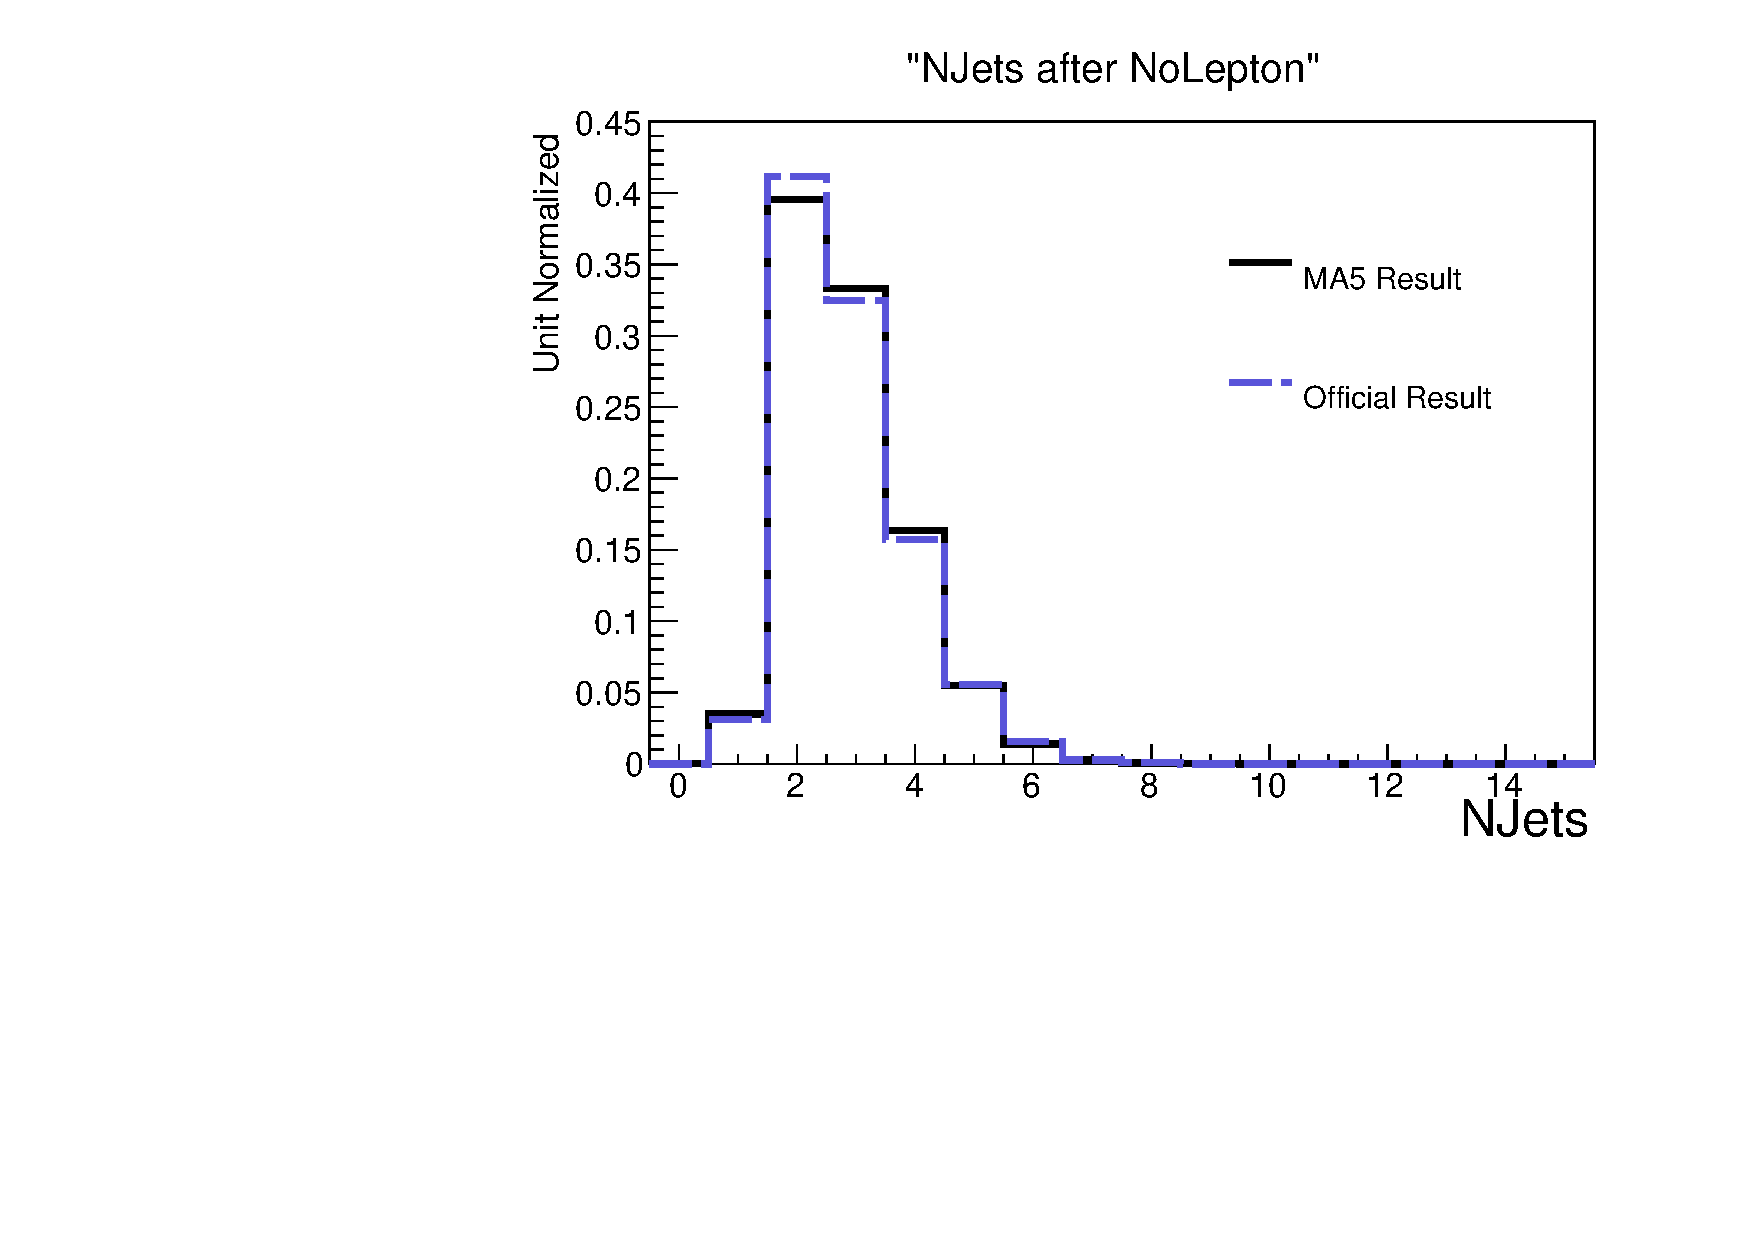
\includegraphics[width=0.5\textwidth]{figures/Appendices/Ma5ValidationSUS13012/T2qq_NJets_after_NoLepton.pdf}
                \label{fig:gull}
        }%
        \hspace{-1 cm}
        ~ %add desired spacing between images, e. g. ~, \quad, \qquad, \hfill etc.
          %(or a blank line to force the subfigure onto a new line)
        \subfloat[]{
                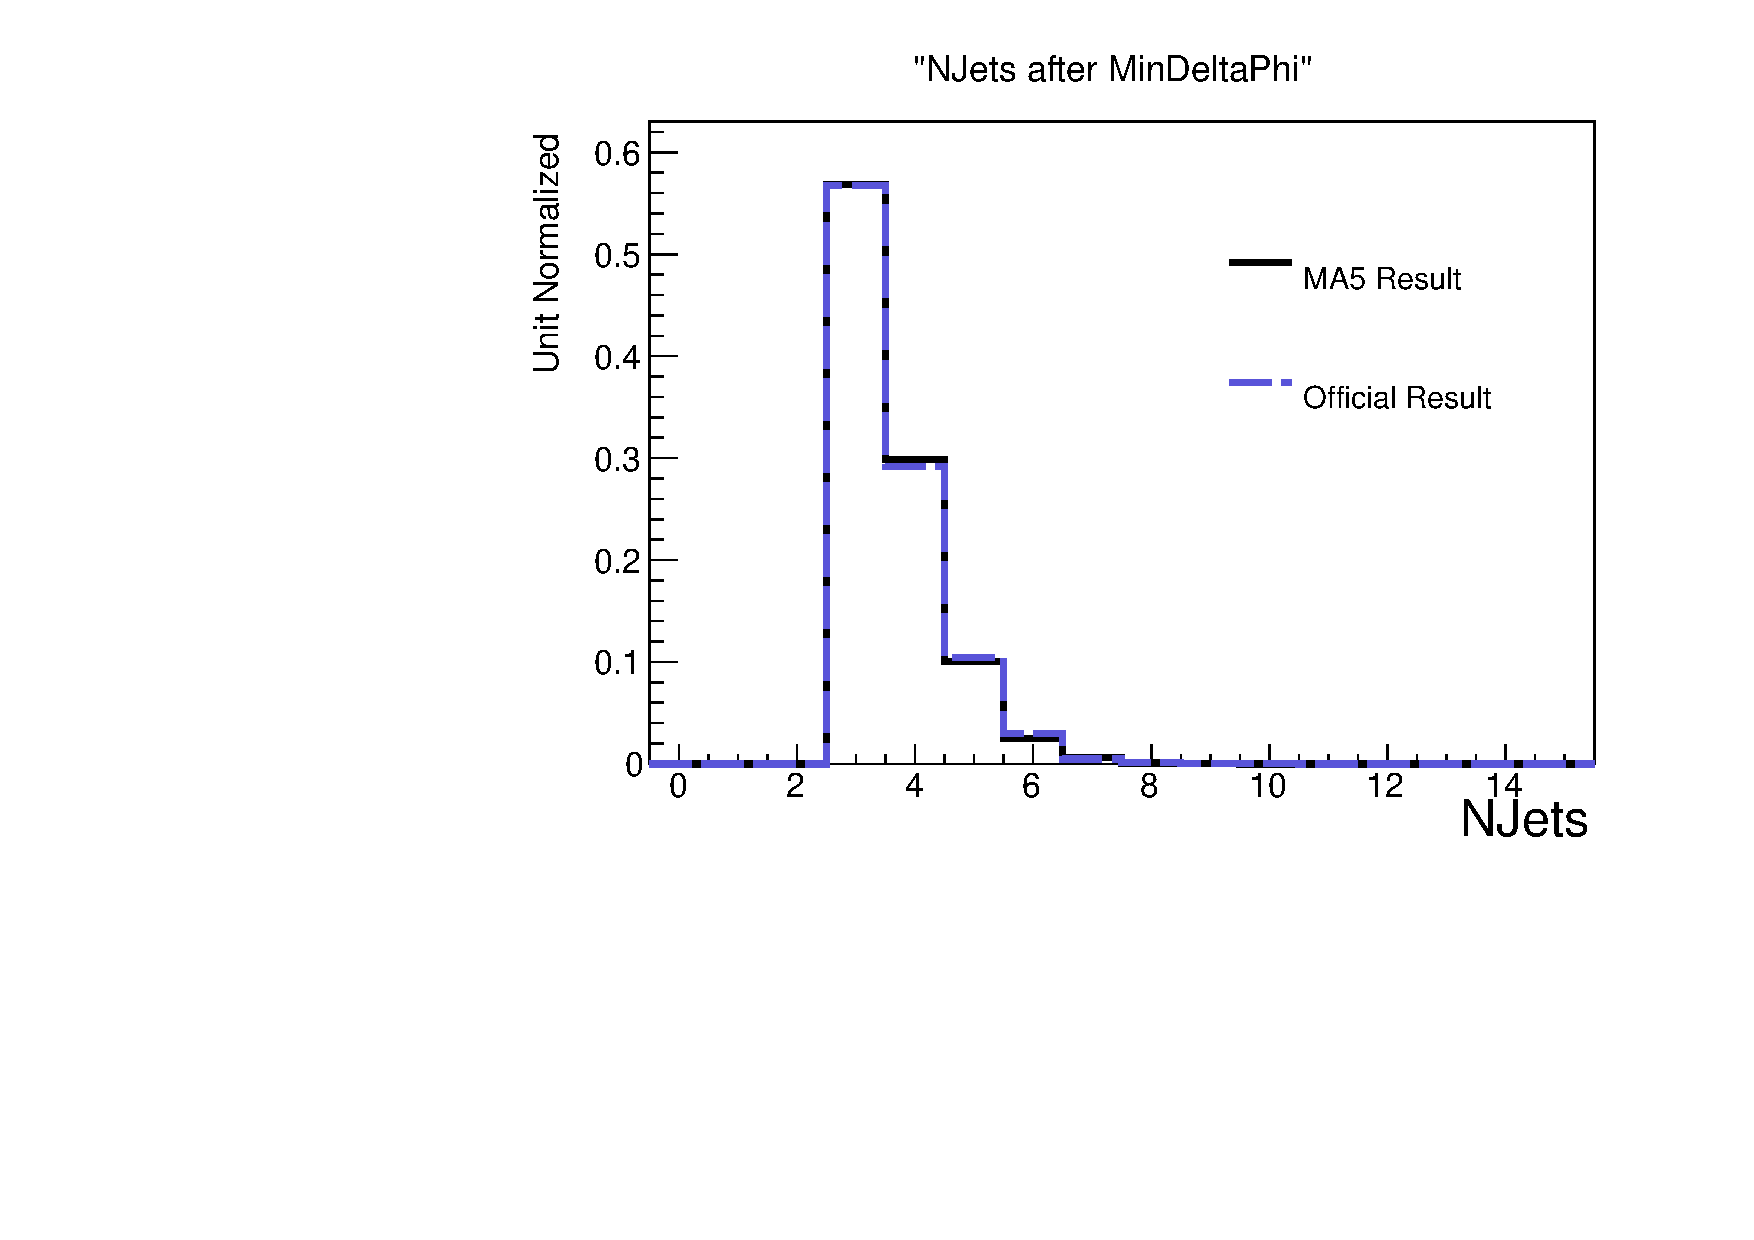
\includegraphics[width=0.5\textwidth]{figures/Appendices/Ma5ValidationSUS13012/T2qq_NJets_after_MinDeltaPhi.pdf}
                \label{fig:tiger}
        }
        \caption{Comparison of the distributions of NJets between the official and our own samples after the ``n-1" cut, Min $\Delta(\phi)$ (left), and after all baseline cuts (right), for the T2qq signal model.}\label{fig:animals}
\end{figure}        
        
        \begin{figure}
        \centering
        \subfloat[]{
        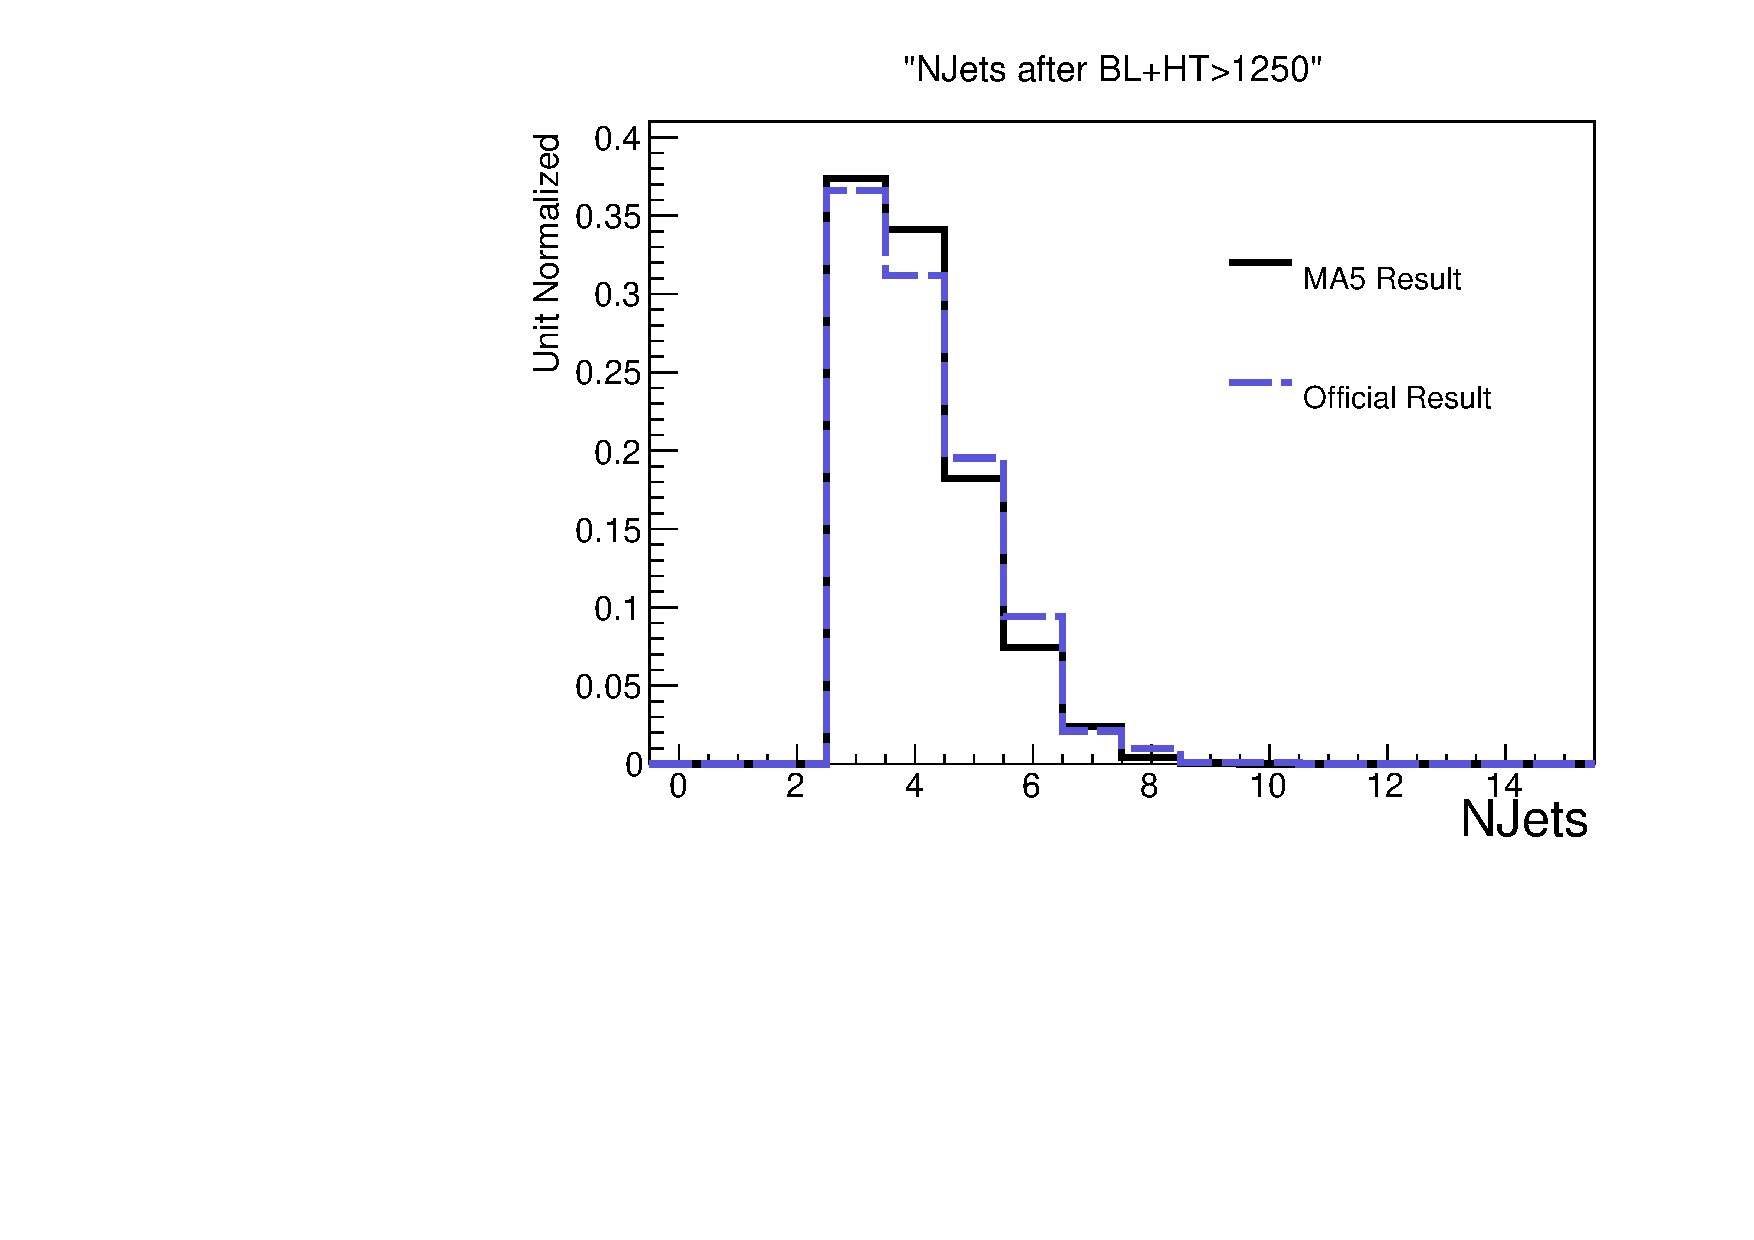
\includegraphics[width=0.5\textwidth]{figures/Appendices/Ma5ValidationSUS13012/T2qq_NJets_after_BL+HT>1250.pdf}
        \label{fig:gull}
        }%
        \hspace{-1 cm}
        ~ %add desired spacing between images, e. g. ~, \quad, \qquad, \hfill etc.
        %(or a blank line to force the subfigure onto a new line)
        \subfloat[]{
        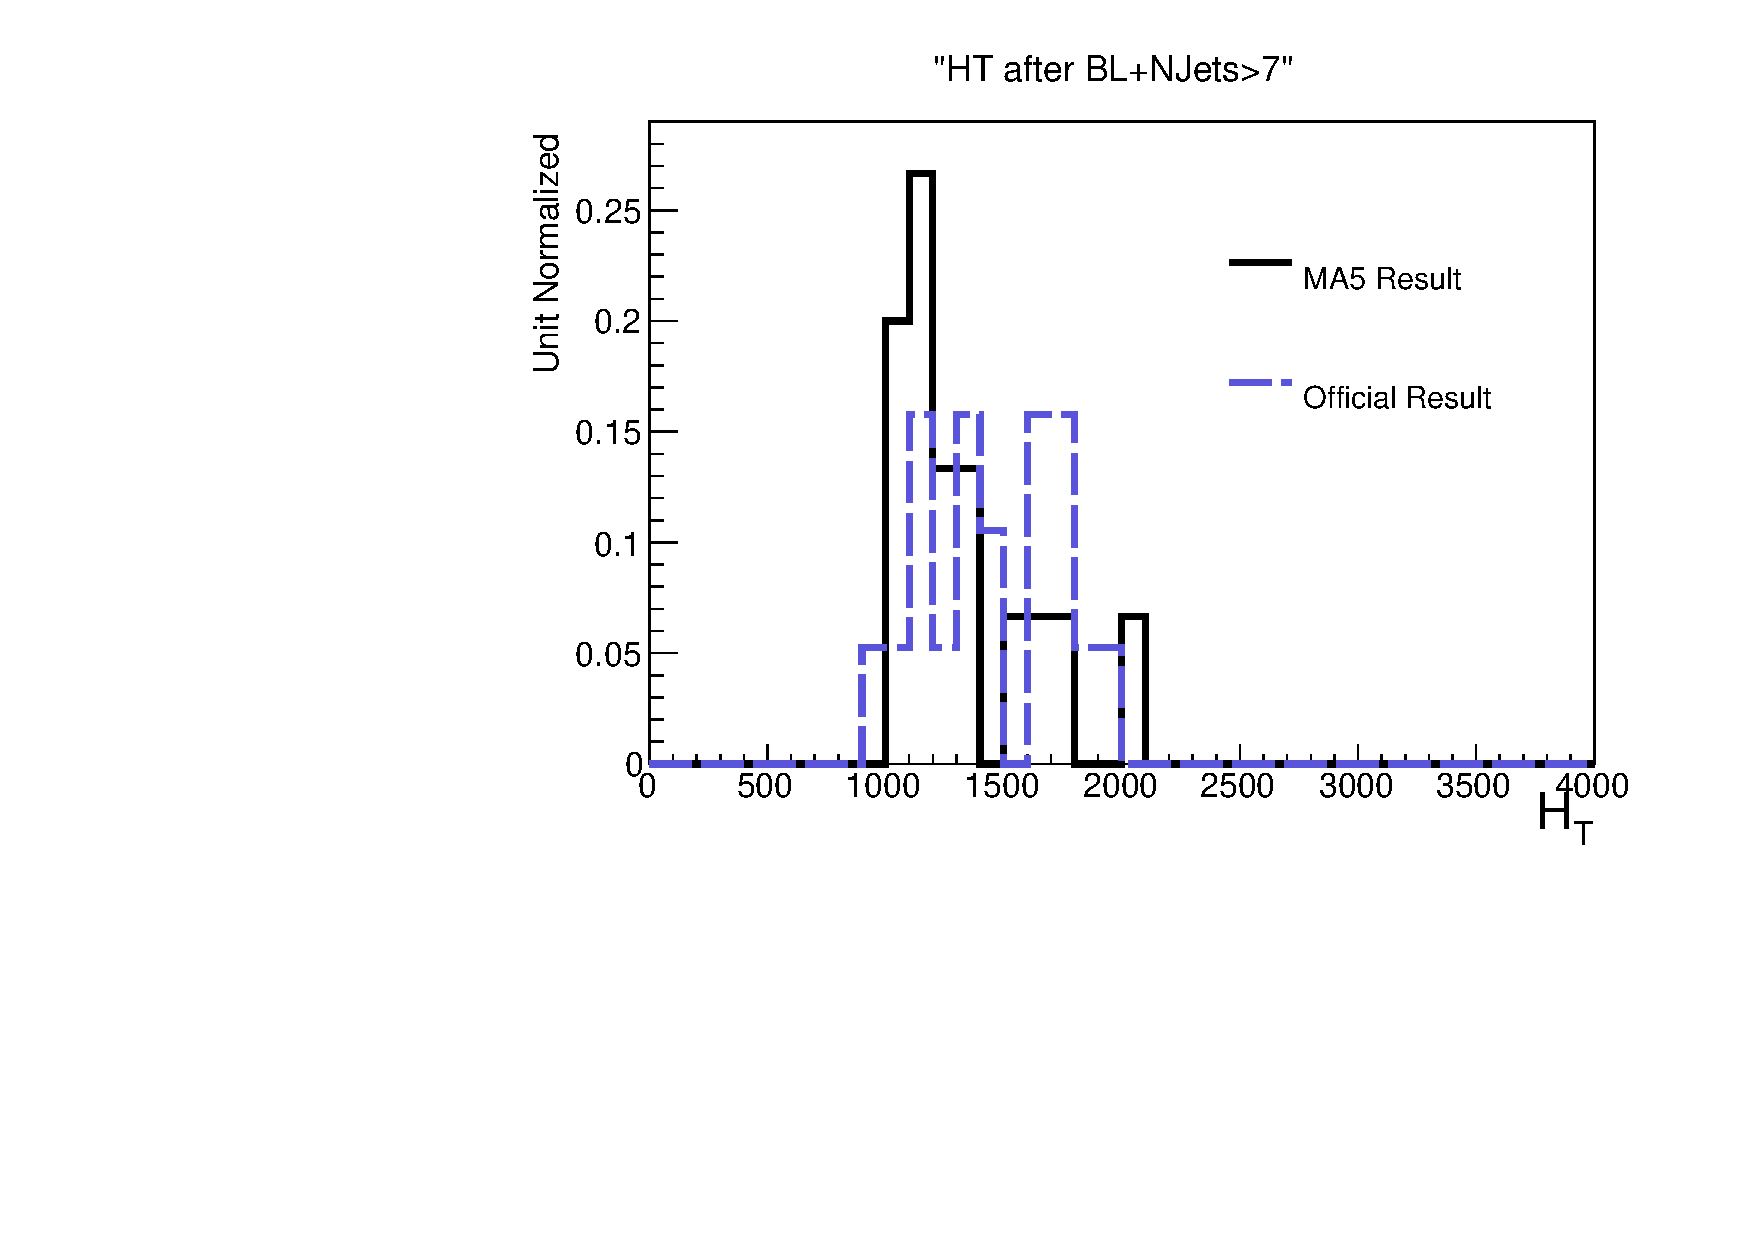
\includegraphics[width=0.5\textwidth]{figures/Appendices/Ma5ValidationSUS13012/T2qq_HT_after_BL+NJets>7.pdf}
        \label{fig:tiger}
        }
        \caption{Additional checks: comparison between ours and the official distributions of NJets after BL+$H_T$$>$1250 cuts (left), and $H_T$ after BL+NJets$>$7 cuts (right), for the T2qq signal model.}
        \label{fig:last}
        \end{figure} 
        
        
\clearpage
%%%%%%%%%%%%%%%%%%%%%%%%%%%%%%%%%%%%%%%%%%%%%%%%%
\subsection{Exclusion Limits}
%%%%%%%%%%%%%%%%%%%%%%%%%%%%%%%%%%%%%%%%%%%%%%%%%

It is also instructive to reproduce the 95\%~CL exclusion lines in the $(m_{\tilde g},\,m_{\tilde\chi^0_1})$ 
and $(m_{\tilde q},\,m_{\tilde\chi^0_1})$ mass planes.  
% for the four benchmark scenarios, T1tttt ($\tilde{g}\to t\bar{t}\chi_{1}^{0}$),
%T2qq ($\tilde{q}\to q \chi_{1}^{0} $), T1qqqq ($\tilde{g}\to q\bar{q}\chi_{1}^{0}$),
%and T5VV ($\tilde{g} \to q\bar{q}V\chi_{1}^{0}$). 
Figure~\ref{fig:limitplots}  shows the limit curves (in red) obtained with our 
{\sc{MadAnalysis}}~5 implementation and using the {\tt{exclusion\_CLs.py}} code described in 
\href{http://arxiv.org/abs/arXiv:1407.3278}{arXiv:1407.3278} 
superimposed on the official CMS exclusion with its $\pm 1\sigma$ theoretical uncertainty (solid and dashed black lines).  For the T1qqqq ($\tilde{g}\to q\bar{q}\chi_{1}^{0}$) and T5VV ($\tilde{g} \to q\bar{q}V\chi_{1}^{0}$) simplified models, the limits are reproduced very well. 
Also for T1tttt ($\tilde{g}\to t\bar{t}\chi_{1}^{0}$) the agreement is reasonably fine. 
For T2qq ($\tilde{q}\to q \chi_{1}^{0} $), however, we encounter a rather erratic behavior for 
LSP masses above about 200--250~GeV.

It should be noted that our limit setting procedure differs from that used by CMS, and so should be 
considered a rough estimate. Our procedure is as follows. For any given point
on the mass plane, the production cross section is taken from the LHC SUSY cross sections twiki 
and the signal acceptance is computed with our {\sc{MadAnalysis}}~5 recast code for the analysis.
Then, the most sensitive signal region (SR), out of the 36 total SRs, is determined based on the 
number of expected signal and background counts. 
Finally, the CLs exclusion value is determined from the expected signal, expected
background, expected uncertainty on the background, and observed counts in the most sensitive
SR. 

The primary difference between our method and that used by CMS is that we consider only the most sensitive SR
in the exclusion calculation, whereas CMS uses all signal regions simultaneously and considers correlations
in the uncertainty between signal regions. This difference introduces a certain volatility in our  
exclusion limits, which can however be mitigated by demanding that jumps in exclsusion between two 
neighbouring points close in mass be not too large. 
As can be seen in Fig.!\ref{fig:limitplots}, we obtain excellent results for the T1qqqq and T5VV scenarios; the 
exclusion curve for T1tttt shows more fluctuations but none the less matches the official result reasonably well. 
The only problematic case is the T2qq topology with LSP masses above 200--250~GeV: here our procedure 
clearly does not well reproduce the official limit curve. To improve the situation, we would need the  
statistical model from CMS for combining  the 36 SRs. Unfortunately, this is currently not available.   

 \begin{figure}
        \centering
        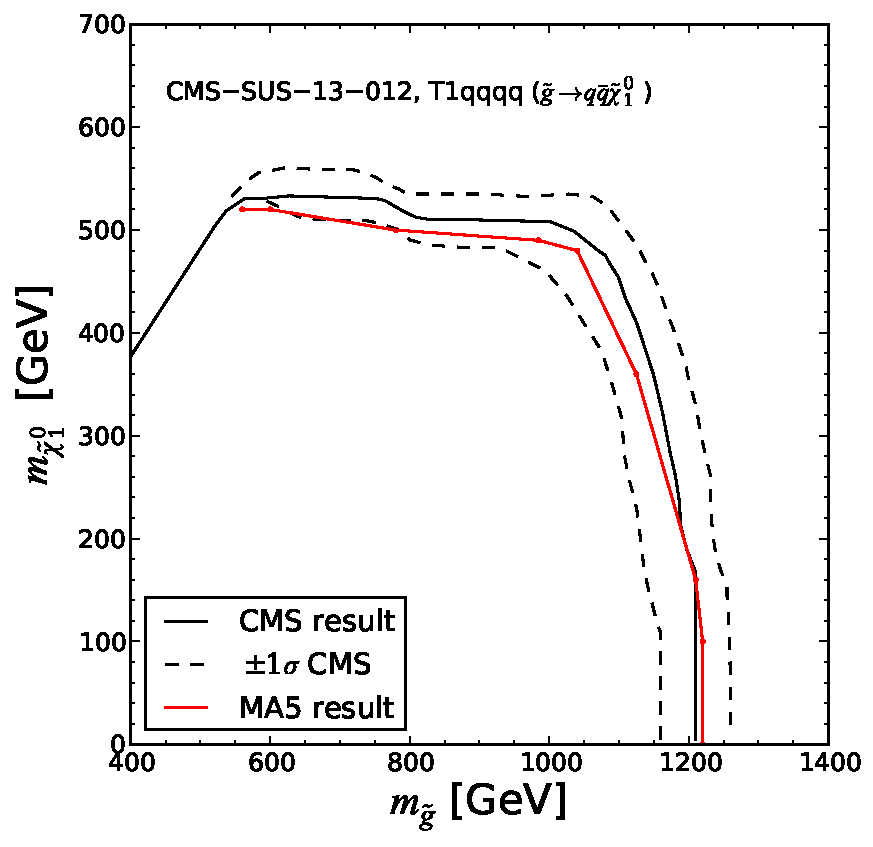
\includegraphics[width=0.48\textwidth]{figures/Appendices/Ma5ValidationSUS13012/cms-012-limit-T1qqqq.pdf}
        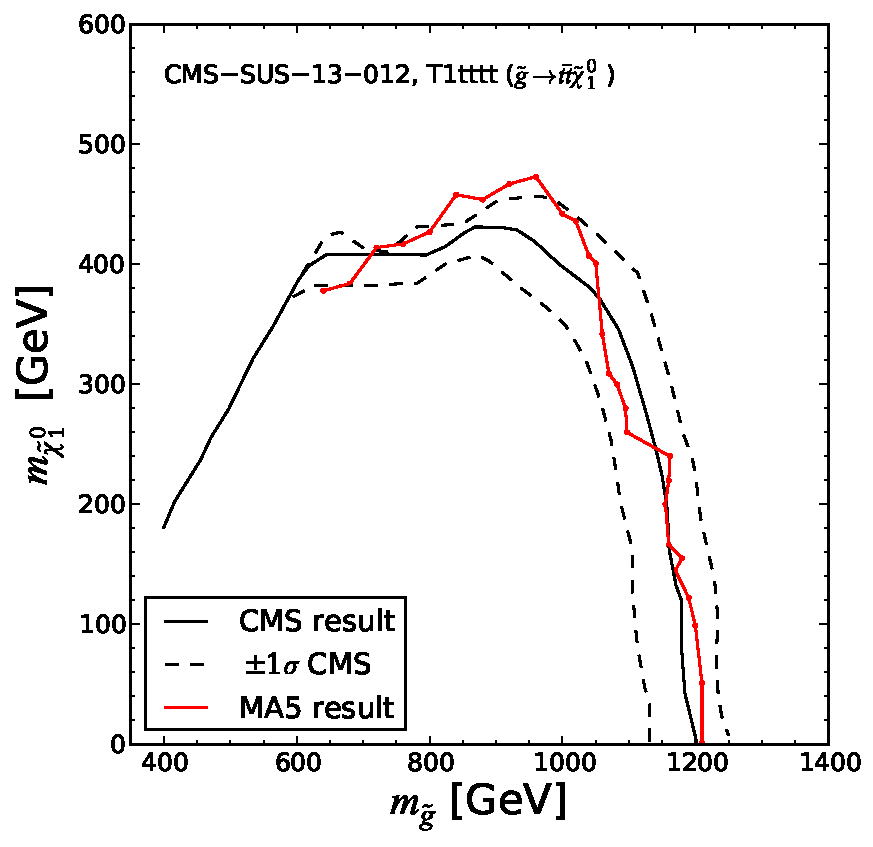
\includegraphics[width=0.48\textwidth]{figures/Appendices/Ma5ValidationSUS13012/cms-012-limit-T1tttt.pdf}\\
        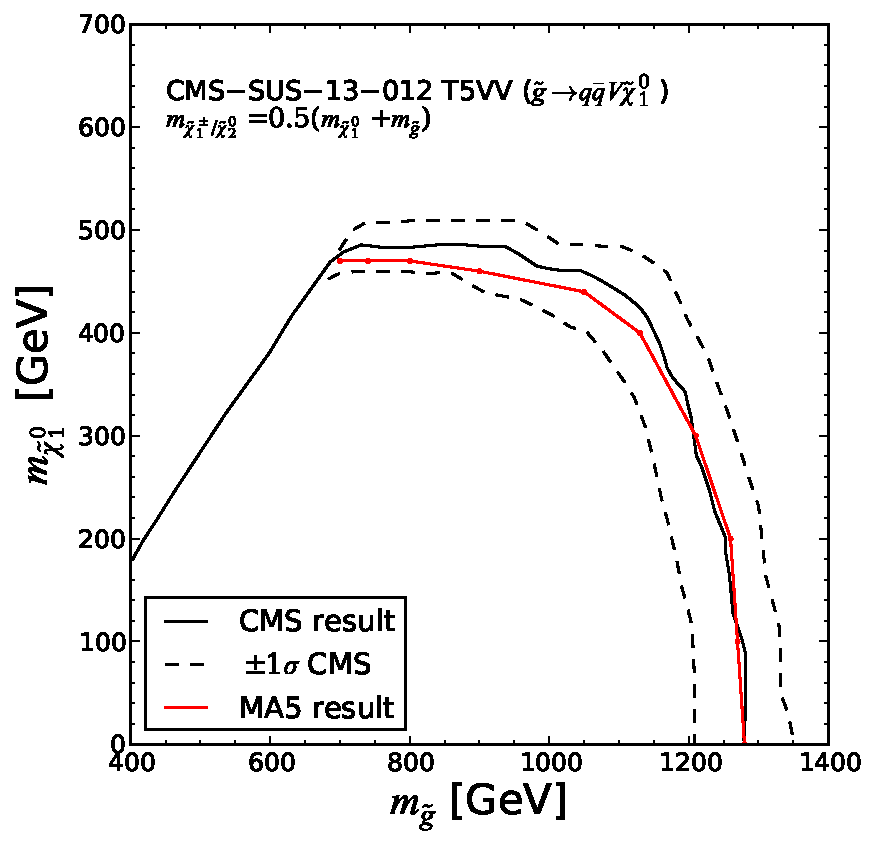
\includegraphics[width=0.48\textwidth]{figures/Appendices/Ma5ValidationSUS13012/cms-012-limit-T5VV.pdf}
        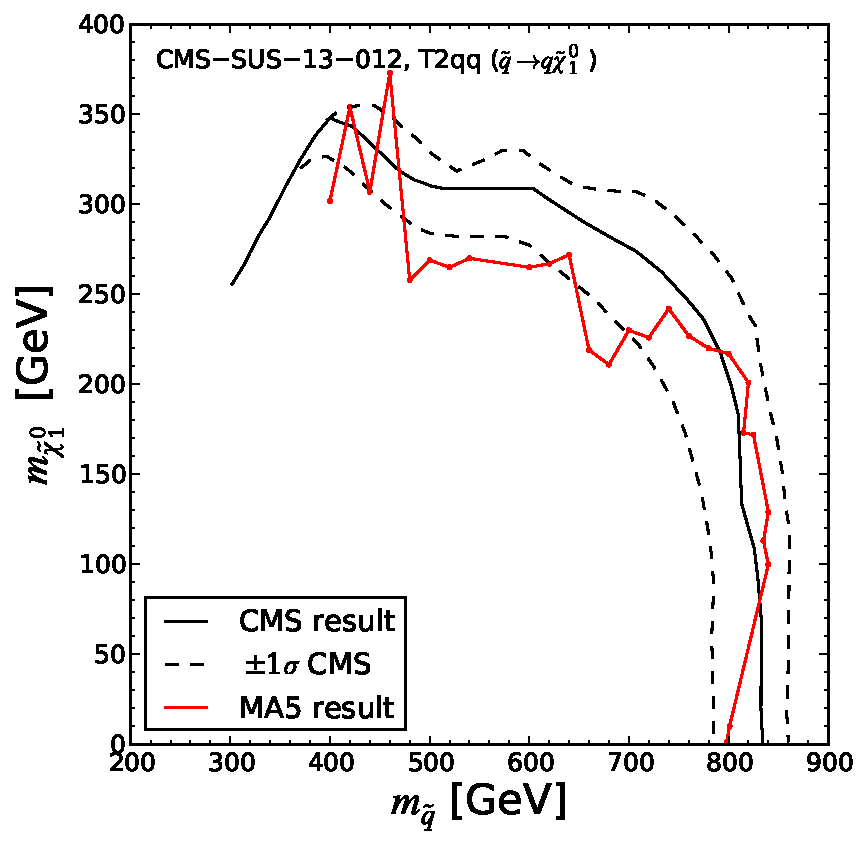
\includegraphics[width=0.48\textwidth]{figures/Appendices/Ma5ValidationSUS13012/cms-012-limit-T2qq.pdf}
\caption{The 95\% CL exclusion limits (in red) reproduced with our {\sc{MadAnalysis}}~5 implementation compared to the official limits (in black) from \href{https://twiki.cern.ch/twiki/bin/view/CMSPublic/PhysicsResultsSUS13012}{CMS-SUS-13-012}. Top left: T1qqqq, top right: T1tttt, bottom left: T5VV, bottom right: T2qq simplified models.
\label{fig:limitplots}}
        \end{figure} 
\FloatBarrier

%%%%%%%%%%%%%%%%%%%%%%%%%%%%%%%%%%%%%%%%%%%%%%%%%%%%%%%%%

The following describes the work documented in \cite{MA5-CMS-SUS-14-001}, in association with the paper~\cite{MA5-CMS-SUS-14-001}.
\textbf{Atmasiddha, Prachi (IISER); Bein, Samuel (Florida State U.)}\\
We present the results of the synchronization of the MA5
implementation of the SUS-14-001 ``top tagging" SUSY search for top squarks.  The
performance of the implementation is evaluated by comparing the
MA5-derived results with a set of cut flow tables and kinematic
distributions provided by CMS for this purpose. The simplified model
T2tt (Fig. \ref{fig:T2tt}) is used as a common benchmark, with values of the masses of the
stop and neutralino taking on a range of values. Two types of
comparisons are given in 
Figs. \ref{table:T2tt-500-125}-\ref{table:T2tt-650-50}: cut flow tables and normalized
kinematic distributions. In some cases the
cut flow tables give the number of events normalized to 100\%; in
other cases the tables are normalized to the cross section times the
integrated luminosity. The normalization convention used by CMS was
followed. Question marks hold the place of values that were not
provided in the CMS cut flow tables.
%%%%%%%%%%%%%%%%%%%%%%%%%%%%%%%%%%%%%%%%%%%%%%%%%
   \begin{figure}
  \centering
    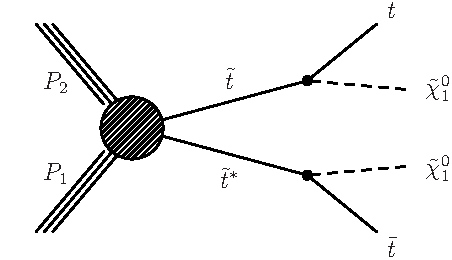
\includegraphics[width=0.5\textwidth]{figures/Appendices/Ma5ValidationSUS13012/T2tt.pdf}
      \caption{Diagram for the T2tt SMS topology. Several mass
        combinations of the stop and LSP are used in the tables below
        as benchmark comparison scenarios.}
      \label{fig:T2tt}
\end{figure}

\begin{table}
    \begin{centering}
    \begin{tabular}{  c | c | c  }
    \hline
    Cut Name & CMS Count(Eff) & MA5 Count(Eff)\\
    \hline
        Event Cleaning & 98.13 (xxx) & 98.13 (xxx)\\
    No Mu & 72.16 (73\%) & 72.21 (73\%)\\
    No Ele & 55.41 (76\%) & 55.50 (76\%)\\
    Njet70$>$1 & 49.55 (89\%) & 50.07 (90\%)\\
    Njet50$>$3 & 31.16 (62\%) & 32.14 (64\%)\\
    Njet30$>$4 & 26.25 (84\%) & 27.10 (84\%)\\
    Min $\Delta(\phi)$ & 22.46 (85\%) & 23.15 (85\%)\\
    Nbjets$>$0 & 19.63 (87\%) & 19.69 (85\%)\\
    MET$>$200 & 12.21 (62\%) & 12.95 (65\%)\\
    Top Reco & - (-) & 5.79 (44\%)\\
    MTsum$>$500 & 4.87 (39\%) & 4.95 (85\%)\\
\hline
    \end{tabular}
    \caption{The acceptance cut flow for the baseline selection in CMS SUS-14-001 for
    model point T2tt-500-125 and the MA5 results are given in column 3.}
    \label{table:T2tt-500-125}
    \end{centering}
    \end{table}

    \begin{table}
    \begin{centering}
    \begin{tabular}{  l | c | c  }
    \hline
    Signal Region Name & CMS & MA5\\
    \hline
    MET200-350,  Nbjets=1 & 1.19 & 1.25\\ 
 \hline 
MET$>$350,  Nbjets=1 & 0.93 & 1.12\\ 
 \hline 
MET200-350,  Nbjets$>$1 & 1.64 & 1.38\\ 
 \hline 
MET$>$350,  Nbjets$>$1 & 1.11 & 1.19\\ 
 \hline 
\hline
    \end{tabular}
    \caption{The signal region (SR) counts in CMS CMS-SUS-14-001 for
    the signal model working pointT2tt-500-125 after all selection has been applied. Column 2 is the CMS account,
    and our own results displayed in column 3. These counts were determined by applying the SR selection to the end of the cut flow featured in table \ref{table:T2tt-500-125}.}
    \end{centering}
    \end{table}



\begin{table}
    \begin{centering}
    \begin{tabular}{  c | c | c  }
    \hline
    Cut Name & CMS Count(Eff) & MA5 Count(Eff)\\
    \hline
        Event Cleaning & 97.44 (xxx) & 97.44 (xxx)\\
    No Mu & 72.5 (74\%) & 71.81 (73\%)\\
    No Ele & 55.55 (76\%) & 54.98 (76\%)\\
    Njet70$>$1 & 52.72 (94\%) & 51.86 (94\%)\\
    Njet50$>$3 & 34.55 (65\%) & 34.66 (66\%)\\
    Njet30$>$4 & 28.49 (82\%) & 28.86 (83\%)\\
    Min $\Delta(\phi)$ & 24.98 (87\%) & 25.22 (87\%)\\
    Nbjets$>$0 & 21.81 (87\%) & 21.67 (85\%)\\
    MET$>$200 & 17.6 (80\%) & 17.73 (81\%)\\
    Top Reco & - (-) & 9.10 (51\%)\\
    MTsum$>$500 & 8.37 (47\%) & 8.52 (93\%)\\
\hline
    \end{tabular}
    \caption{The acceptance cut flow for the baseline selection in CMS SUS-14-001 for
    model point T2tt-650-25 and the MA5 results are given in column 3.}
    \label{table:T2tt-650-25}
    \end{centering}
    \end{table}

    \begin{table}
    \begin{centering}
    \begin{tabular}{  l | c | c  }
    \hline
    Signal Region Name & CMS & MA5\\
    \hline
    MET200-350,  Nbjets=1 & 1.06 & 0.91\\ 
 \hline 
MET$>$350,  Nbjets=1 & 2.49 & 2.93\\ 
 \hline 
MET200-350,  Nbjets$>$1 & 1.34 & 1.24\\ 
 \hline 
MET$>$350,  Nbjets$>$1 & 3.48 & 3.43\\ 
 \hline 
\hline
    \end{tabular}
    \caption{The signal region (SR) counts in CMS CMS-SUS-14-001 for
    the signal model working pointT2tt-650-25 after all selection has been applied. Column 2 is the CMS account,
    and our own results displayed in column 3. These counts were determined by applying the SR selection to the end of the cut flow featured in table \ref{table:T2tt-650-25}.}
    \end{centering}
    \end{table}


\begin{table}
    \begin{centering}
    \begin{tabular}{  c | c | c  }
    \hline
    Cut Name & CMS Count(Eff) & MA5 Count(Eff)\\
    \hline
        Event Cleaning & 15662.0 (xxx) & 15662.0 (xxx)\\
    No Mu & - (-) & 11568.97 (73\%)\\
    No Ele & 8802.0 (56\%) & 8927.82 (77\%)\\
    Njet70$>$1 & - (-) & 7380.74 (82\%)\\
    Njet50$>$3 & - (-) & 4350.13 (58\%)\\
    Njet30$>$4 & 3113.0 (35\%) & 3653.80 (83\%)\\
    Min $\Delta(\phi)$ & 2205.0 (70\%) & 2972.08 (81\%)\\
    Nbjets$>$0 & 2200.0 (99\%) & 2539.64 (85\%)\\
    MET$>$200 & - (-) & 1010.90 (39\%)\\
    Top Reco & - (-) & 314.46 (31\%)\\
    MTsum$>$500 & 182.9 (8\%) & 213.18 (67\%)\\
\hline
    \end{tabular}
    \caption{The acceptance cut flow for the baseline selection in CMS SUS-14-001 for
    model point T2tt-350-0 and the MA5 results are given in column 3.}
    \label{table:T2tt-350-0}
    \end{centering}
    \end{table}

    \begin{table}
    \begin{centering}
    \begin{tabular}{  l | c | c  }
    \hline
    Signal Region Name & CMS & MA5\\
    \hline
    MET200-350,  Nbjets=1 & - & 95.08\\ 
 \hline 
MET$>$350,  Nbjets=1 & - & 13.66\\ 
 \hline 
MET200-350,  Nbjets$>$1 & - & 90.88\\ 
 \hline 
MET$>$350,  Nbjets$>$1 & 7.5 & 13.55\\ 
 \hline 
\hline
    \end{tabular}
    \caption{The signal region (SR) counts in CMS CMS-SUS-14-001 for
    the signal model working pointT2tt-350-0 after all selection has been applied. Column 2 is the CMS account,
    and our own results displayed in column 3. These counts were determined by applying the SR selection to the end of the cut flow featured in table \ref{table:T2tt-350-0}.}
    \end{centering}
    \end{table}
    
   \begin{figure}
  \caption{MA5 and CMS unit-normalized kinematic distributions after the baseline
    selection for the T2tt working point (350,0).}
  \centering
    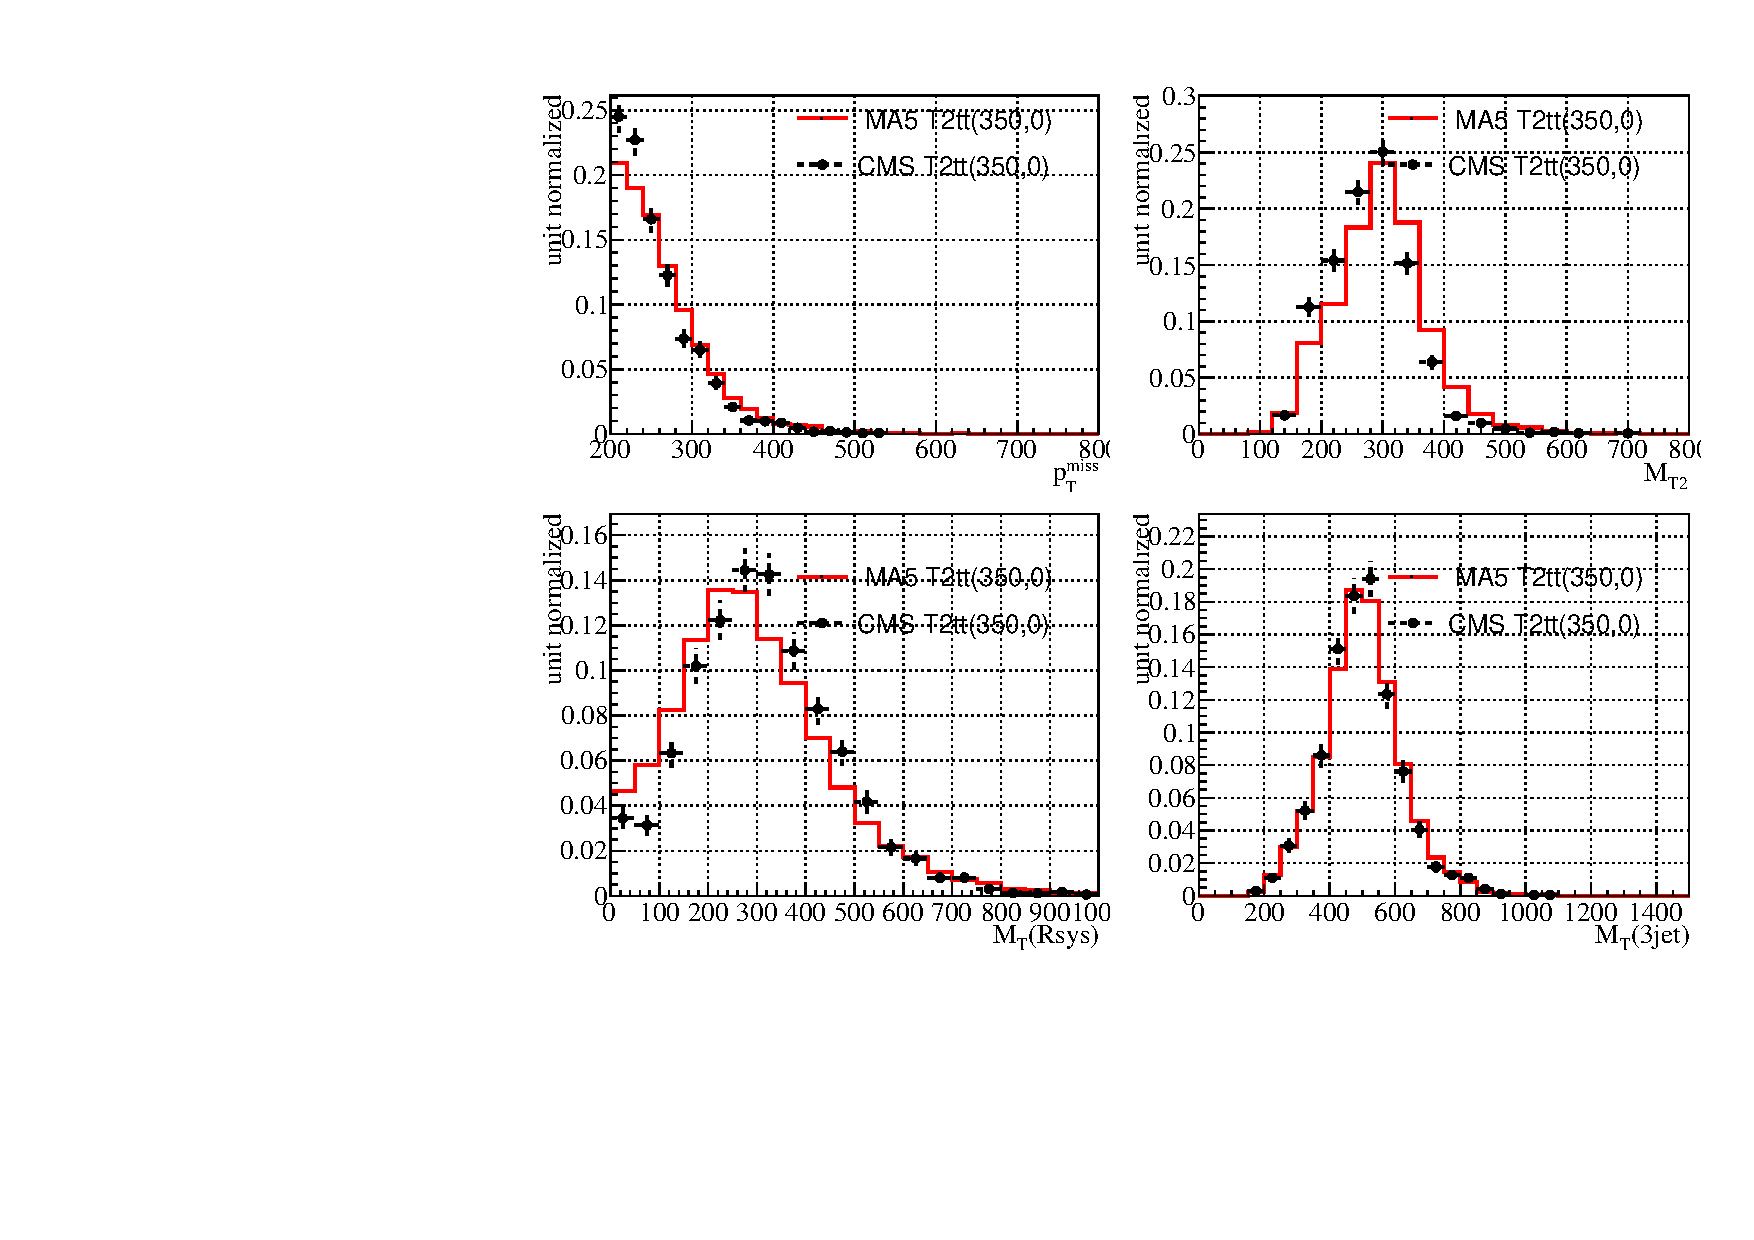
\includegraphics[width=\textwidth]{figures/Appendices/Ma5ValidationSUS13012/T2tt-350-0.pdf}
\end{figure}



\begin{table}
    \begin{centering}
    \begin{tabular}{  c | c | c  }
    \hline
    \hline
    Cut Name & CMS Count(Eff) & MA5 Count(Eff)\\
    \hline
        Event Cleaning & 1660.0 (xxx) & 1660.0 (xxx)\\
    No Mu & - (-) & 1229.14 (74\%)\\
    No Ele & 927.0 (55\%) & 942.80 (76\%)\\
    Njet70$>$1 & - (-) & 856.80 (90\%)\\
    Njet50$>$3 & - (-) & 551.71 (64\%)\\
    Njet30$>$4 & 419.0 (45\%) & 468.27 (84\%)\\
    Min $\Delta(\phi)$ & 360.0 (85\%) & 400.29 (85\%)\\
    Nbjets$>$0 & 314.0 (87\%) & 341.67 (85\%)\\
    MET$>$200 & - (-) & 229.78 (67\%)\\
    Top Reco & - (-) & 105.02 (45\%)\\
    MTsum$>$500 & 85.9 (27\%) & 90.82 (86\%)\\
\hline
    \hline
    \end{tabular}
    \caption{The acceptance cut flow for the baseline selection in CMS SUS-14-001 for
    model point T2tt-500-100 and the MA5 results are given in column 3.}
    \label{table:T2tt-500-100}
    \end{centering}
    \end{table}

    \begin{table}
    \begin{centering}
    \begin{tabular}{  l | c | c  }
    \hline
        \hline
    Signal Region Name & CMS & MA5\\
    \hline
    MET200-350,  Nbjets=1 & - & 21.48\\ 
 \hline 
MET$>$350,  Nbjets=1 & - & 20.52\\ 
 \hline 
MET200-350,  Nbjets$>$1 & - & 25.31\\ 
 \hline 
MET$>$350,  Nbjets$>$1 & 19.8 & 23.50\\ 
 \hline 
\hline
    \end{tabular}
    \caption{The signal region (SR) counts in CMS CMS-SUS-14-001 for
    the signal model working pointT2tt-500-100 after all selection has been applied. Column 2 is the CMS account,
    and our own results displayed in column 3. These counts were determined by applying the SR selection to the end of the cut flow featured in table \ref{table:T2tt-500-100}.}
    \end{centering}
    \end{table}
    
   \begin{figure}
  \caption{MA5 and CMS unit-normalized kinematic distributions after the baseline
    selection for the T2tt working point (500,100).}
  \centering
    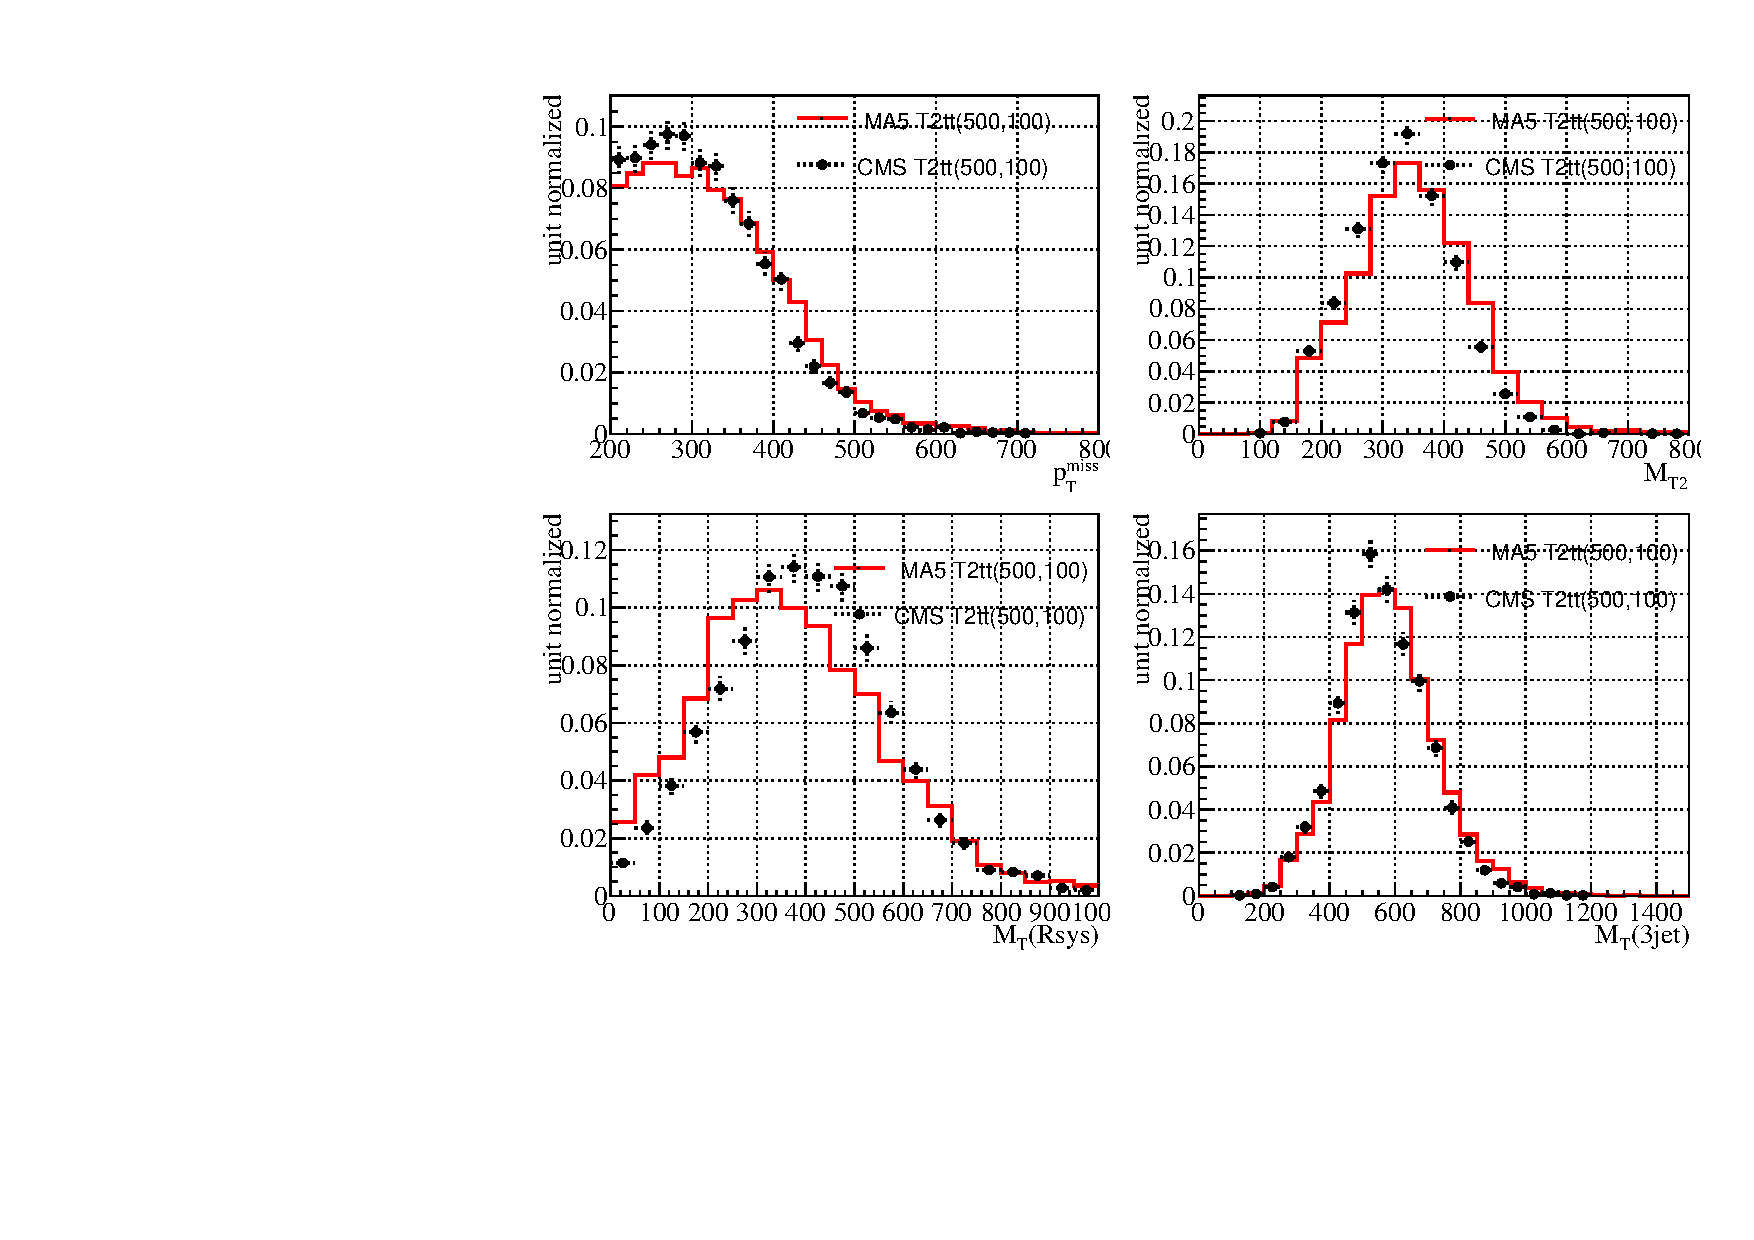
\includegraphics[width=\textwidth]{figures/Appendices/Ma5ValidationSUS13012/T2tt-500-100.pdf}
\end{figure}


\begin{table}
    \begin{centering}
    \begin{tabular}{  c | c | c  }
    \hline
        \hline
    Cut Name & CMS Count(Eff) & MA5 Count(Eff)\\
    \hline
        Event Cleaning & 270.8 (xxx) & 270.8 (xxx)\\
    No Mu & - (-) & 199.25 (73\%)\\
    No Ele & 152.0 (56\%) & 152.26 (76\%)\\
    Njet70$>$1 & - (-) & 143.65 (94\%)\\
    Njet50$>$3 & - (-) & 95.87 (66\%)\\
    Njet30$>$4 & 75.0 (49\%) & 79.95 (83\%)\\
    Min $\Delta(\phi)$ & 66.0 (88\%) & 69.84 (87\%)\\
    Nbjets$>$0 & 58.0 (87\%) & 59.99 (85\%)\\
    MET$>$200 & - (-) & 48.58 (80\%)\\
    Top Reco & - (-) & 25.36 (52\%)\\
    MTsum$>$500 & 22.7 (39\%) & 23.71 (93\%)\\
\hline
    \end{tabular}
    \caption{The acceptance cut flow for the baseline selection in CMS SUS-14-001 for
    model point T2tt-650-50 and the MA5 results are given in column 3.}
    \label{table:T2tt-650-50}
    \end{centering}
    \end{table}

    \begin{table}
    \begin{centering}
    \begin{tabular}{  l | c | c  }
    \hline
    Signal Region Name & CMS & MA5\\
    \hline
    MET200-350,  Nbjets=1 & - & 2.77\\ 
 \hline 
MET$>$350,  Nbjets=1 & - & 8.08\\ 
 \hline 
MET200-350,  Nbjets$>$1 & - & 3.35\\ 
 \hline 
MET$>$350,  Nbjets$>$1 & 9.3 & 9.49\\ 
 \hline 
\hline
    \end{tabular}
    \caption{The signal region (SR) counts in CMS CMS-SUS-14-001 for
    the signal model working pointT2tt-650-50 after all selection has been applied. Column 2 is the CMS account,
    and our own results displayed in column 3. These counts were determined by applying the SR selection to the end of the cut flow featured in table \ref{table:T2tt-650-50}.}
    \end{centering}
    \end{table}


   \begin{figure}
  \caption{MA5 and CMS unit-normalized kinematic distributions after the baseline
    selection for the T2tt working point (650,50).}
  \centering
    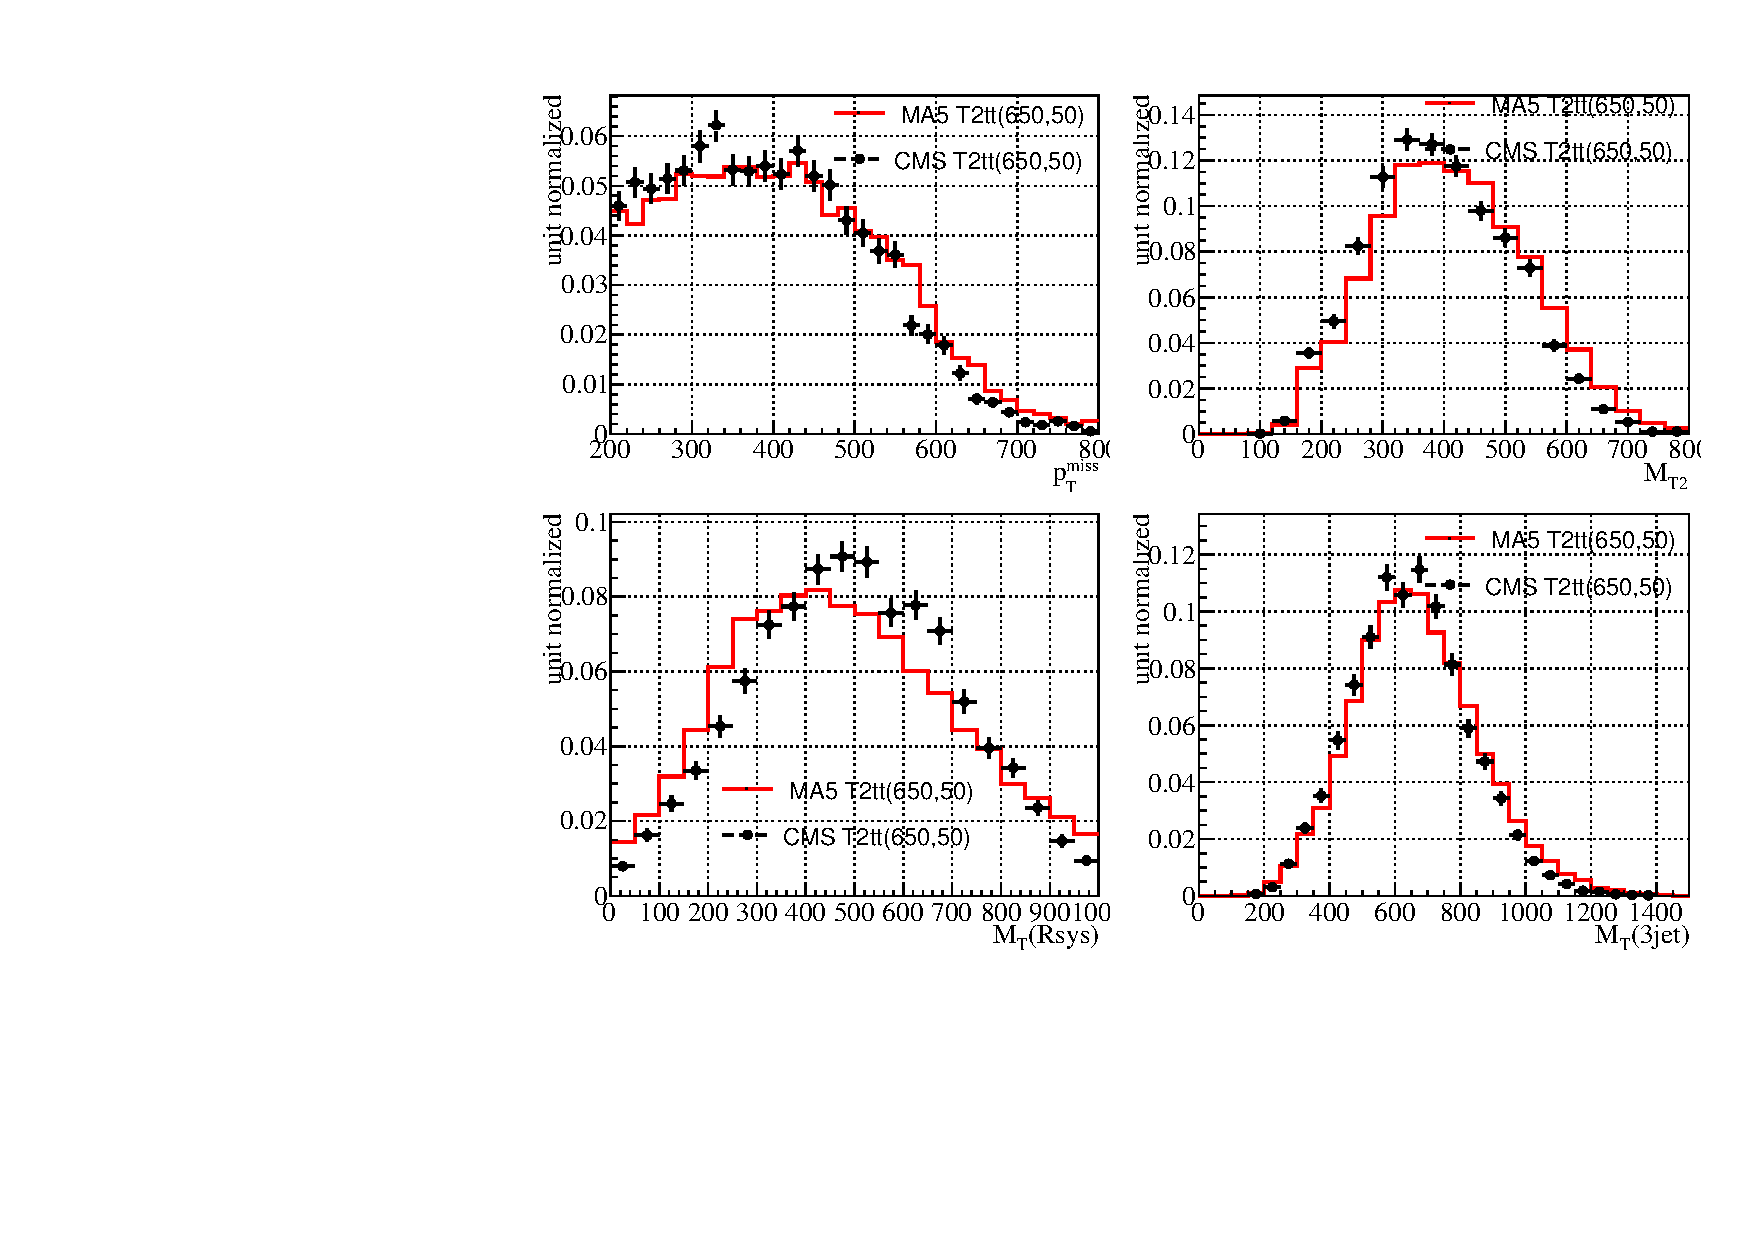
\includegraphics[width=\textwidth]{figures/Appendices/Ma5ValidationSUS13012/T2tt-650-50.pdf}
\end{figure}

%%%%%%%%%%%%%%%%%%%%%%%%%%%%%%%%%%%%%%%%%%%%%%%%%
